% \begin{savequote}[8cm]
% Alles Gescheite ist schon gedacht worden.\\
% Man muss nur versuchen, es noch einmal zu denken.

% All intelligent thoughts have already been thought;\\
% what is necessary is only to try to think them again.
%   \qauthor{--- Johann Wolfgang von Goethe \cite{von_goethe_wilhelm_1829}}
% \end{savequote}

\chapter{\label{ch:spf}A Possibility Frontier Approach to Diverse Talent Selection}

\minitoc

\section{Abstract}
We hypothesize that the complexity of selecting personnel in a way that jointly optimizes for talent (performance on an ability measure) and diversity impedes organizations from meeting their diversity, equity, and inclusion goals. To formalize this, we prove that maximizing cohort diversity is computationally complex and incorporate this complexity into a selection model by adding computational costs. To test the model's predictions, we construct an algorithm to estimate the diversity-talent frontier, which we apply to data from a scholarship and talent investment program. We find that finalists could have been 13\% (15.6\%) more diverse (more talented) without reducing talent (diversity). We also show that the program selected a significantly more diverse and talented cohort after we provided them with a frontier estimate. We conclude by using program data to demonstrate how the frontier estimation procedure can be used to evaluate the efficacy of alternative screening approaches. This reveals that if the program had screened on IQ, they would have significantly reduced diversity and overlooked many of the most talented applicants.

\section{Introduction}\label{sec:introduction}
The rise of diversity, equity, and inclusion initiatives suggests that various organizations (e.g. schools, firms, social impact programs, etc.) are genuinely interested in selecting for diverse talent. This is driven, at least in part, by recent declines in discrimination \cite{hsieh2019allocation}, increases in the perceived return to diversity \cite{deming2017growing, page2019diversity, noray2023systemic}, and increased social pressure for demographic representation \cite{minkin2023diversity}. In this paper, we hypothesize that the complexity of simultaneously optimizing for talent and diversity leads organizations (even well-intentioned ones) to select within their feasible talent-diversity frontier \cite{nemhauser1978analysis, huppenkothen2020entrofy}. This paper tests this hypothesis by demonstrating and incorporating this complexity into a simple model of cohort selection and testing the empirical predictions of the model using data from a high-profile scholarship and talent investment program. 

We begin by developing a simple model of cohort selection. Organizations receive $N$ applications and must select $n<N$ individuals to construct a cohort from the total set of potential cohorts, each of which is indexed by $c$. The organization seeks to maximize a preference function that is increasing in both a cohort's talent (e.g., the mean performance on an ability measure) and a cohort's diversity (e.g., an inverse distance to a set of target proportions of demographic groups). We then prove that this problem, though simple to state, is computationally complex. This is for two intuitive reasons. First, an individual's contribution to the diversity of the cohort depends on who else will be part of the cohort. Thus, to determine which cohort is the smallest distance from the predefined "ideal" diverse cohort, every possible cohort needs to be assessed. Second, when diversity preferences are for representation of at least two non-mutually exclusive identities (e.g. ethnic minorities and women), optimally selecting members of one group constrains your ability to do the same for the other group. Formally, we show that maximizing functions on subsets is in general non-polynomial. We then show that, when we restrict our attention to functions formalizing diversity as organizations measure it, the `Vertex Cover' problem, known to be $\mathpzc{NP}$-hard, reduces to diversity maximization. This implies that calculating the maximal diversity conditional on cohort performance (what we refer to as the Selection Possibilities Frontier, or SPF) is also $\mathpzc{NP}$-hard. Selecting on the SPF, then, is likely prohibitively costly for many organizations. 

To account for this complexity, we augment our model of cohort selection by forcing organizations to incur a computational marginal cost for each unit of increased cohort diversity. This represents the fact that, to find a more diverse cohort, one must engage in the laborious process of composing potential cohorts and comparing them. This is in sharp contrast to finding more talented cohorts, which is comparatively simple -- and, therefore, modeled as costless -- because each individual's contribution to cohort talent is unrelated to the remainder of the cohort. This simple model has two implications: (1) organizations will tend to select sub-optimal (i.e. non-first-best) cohorts and (2) organizations will improve on both performance and diversity if the gain access to a technology that reduces this computational marginal cost. 

We then develop an algorithm that can estimate the SPF in polynomial time. To do this we use optimization theory to show that a greedy algorithm can be used to approximate the maximal diversity as long as the function that maps cohorts to diversity scores is submodular, monotonic, and non-negative \cite{krause2014submodular, huppenkothen2020entrofy}. We then construct a formal algorithmic procedure that uses the greedy method to maximize a weighted sum of cohort diversity and cohort performance. Finally, we exploit the observation that the SPF is isomorphic to the diversity and talent levels of the set of cohorts that maximize the weighted sum for some value of the weights. Thus, we apply this procedure repeatedly using different weights to estimate the entire SPF. We also derive bounds for each estimated point on the SPF. 

Next, we turn to the empirical component of the paper where we test our model's predictions by applying the SPF estimate to selection data from a high-profile scholarship and talent investment program. The program aims to find talented high-schoolers from around the world and invest in them so they can realize their full career potential. The program provides winners with various benefits such as college scholarships, career support, and networking opportunities. When making decisions about which applicants to choose, the program weighs both cohort composition (i.e. diversity) and the cohort talent. For diversity, the program has clear preferences that the cohort be as close as possible to explicit proportions of various demographic groups defined along various dimensions such as gender, socioeconomic status, global region of origin, and country of origin. On the talent dimension, applicants are judged by experts primarily on the quality of concrete projects designed to showcase their potential (e.g. robots, mobile applications, engineering blueprints, etc.).

We start our empirical analysis by estimating SPFs for the first two consecutive application cycles and using them to test whether the program could have selected cohorts more efficiently. We find that, in cycle 1, the set of finalists could have been $18.5\%$ more diverse without any reduction in performance and $17.8\%$ higher-performing without any reduction in diversity. Similarly, in cycle 2, the finalists could have been $14.6\%$ more diverse without any reduction in performance and $24.1\%$ higher-performing without any reduction in diversity. Thus, both cohorts chosen were non-first-best as measured by the program's definitions of diversity and performance. We also show that in cycle 3, when the program was given access to the SPF, they significantly improved the efficiency of their selection process, choosing a cohort that was more diverse, higher performing, and essentially on the estimated SPF. This provides suggestive evidence that the SPF aided their decision-making and allowed them to better optimize in the face of a complex choice.

We conclude our empirical analysis by using our SPF estimation procedure to evaluate the efficacy of alternative screening and selection methods. To do this, we leverage two unique aspects of the program. First, the program collects both traditional merit-based measures -- including cognitive tests, written essays, and referring organizations -- as well as non-traditional measures -- including peer reviewed video essays, gamified skill tests, and application platform behaviors. Second, the program engaged in effectively no screening before receiving concrete projects from applicants, making it possible to estimate valid counterfactual diversity and performance of cohorts had they been screened in different ways. Leveraging these features, we find three key results. First, selecting only on the basis of cognitive ability or traditional metrics would have improved cohort performance relative to random selection, but would significantly restricted the program from reaching its diversity goals. By contrast, selecting only on peer reviews performs similarly on performance but improves diversity substantially. Second, all alternative selection methods we explore result in selecting cohorts well within the SPF and, therefore, leave substantial diversity and performance gains on the table. And third, the trade-off implied by the SPF between talent and diversity is steeper if traditional measures are used to measure talent than if applicant projects are used. 

This paper contributes to a growing economics literature studying the influence and potential of algorithms. Most research in this area has focused on measuring the effects of AI tools both at the economy-wide ("macro") level \cite{acemoglu2022automation,babina2024artificial,calvino2023portrait,zolas2021advanced,webb2019impact} and in more specific ("micro") contexts like bail decisions and radiology \cite{albright2023hidden,kleinberg2015prediction,stevenson2019algorithmic,angelova2023algorithmic,imai2023experimental,grimon2022impact,noy2023experimental,brynjolfsson2023generative,bundorf2019humans, mullainathan2019machine, ribers2020machine, agarwal2023combining}. This paper is more closely related to the small subset of this work that \emph{develops} AI tools to improve or assess human problem-solving in some respect.\footnote{Though small in economics, there is a larger literature in computer science that focuses on developing algorithmic tools to replace or improve humans' capacity to solve problems. Most closely related to this paper are machine systems that help organizations select in ways that are "unbiased" \cite{tambe2019artificial,raghavan2020mitigating} or account for "diversity" \cite{gillet2011diversity,huppenkothen2020entrofy}. Our paper differs from these because we account for trade-offs between diversity and other desiderata (e.g. talent, productivity, etc.).}  This includes work that develops methods to compare the efficacy of human vs. AI predictions \cite{kleinberg2018human,rambachan2024identifying} and several papers that develop algorithms specifically to improve the selection or assignment of personnel \cite{li2020hiring,bergman2021seven,kleinberg2018algorithmic,huppenkothen2020entrofy}. Our paper contributes to this literature by developing and applying algorithmic tools to the increasingly relevant diverse talent selection problem. 

Our paper is closely related to \citeA{kleinberg2018algorithmic}, which introduces an algorithm that colleges can use to calculate the most meritorious cohort at any threshold of representation for a single underrepresented group. Their algorithm is straightforward: define a minority group (e.g. black applicants) and the corresponding majority group (e.g. white applicants), rank applicants within each group by measure of merit (e.g. test scores, predicted college performance, etc.), set a threshold for the proportion of those selected who should be part of the minority group, select minority group members from the highest ranking down until the threshold is met, and finally, select the majority group members from the highest ranking down until all slots are filled. Though effective, this procedure only works when the organization aims to represent mutually exclusive minority groups. If diversity preferences are instead for representation of multiple non-mutually exclusive groups (e.g., female applicants and black applicants), this strategy no longer works. This paper relaxes this assumption and outlines the conditions under which the diversity-performance frontier can be estimated regardless of the number or type of identity characteristics organizations seek to represent.

This paper is also related to the growing economics literature on the impact of new screening technologies on the productivity and diversity of the personnel that organizations select. An early paper on this topic is \citeA{autor2008does}, which shows that adding personality tests to the job applicant screening process in a national retail firm increased the productivity of selected workers without reducing minority representation among hires. More recently, \citeA{li2020hiring} demonstrate that, within a Fortune 500 tech company, diversity and productivity of hires can be improved by using exploration-based applicant screening algorithms that recommend applicants with rare sets of characteristics at higher rates in order to improve noisy predictions and, therefore, learn how to find promising applicants from atypical backgrounds. Similarly, \citeA{bergman2021seven} show that, across seven colleges, using a prediction algorithm instead of a test to decide whether to place students into remedial classes improves student performance and increases minority representation in college-level (non-remedial) courses. Our paper adds to this literature in two ways. First, rather than focusing on comparing a new screening method to the status quo, this paper develops a procedure for estimating the diversity-performance frontier itself. Second, leveraging the novel design of the scholarship's application process in combination with our estimate of the SPF, we provide new evidence on the efficacy of screening on traditional "merit" measures. 

This paper is also related to work across fields defining fairness and equity in talent selection. Much of this work builds on the \emph{similar treatment principle} whereby individuals who perform similarly on some dimension(s) are treated equally in selection \cite{dwork2012fairness}.\footnote{Though not generally mentioned in this literature, the similar treatment principle is the normative basis on which differential treatment of demographic groups in audit studies is deemed wrong.} This approach has been criticized, however, on the grounds that in circumstances when performance and demographic factors are correlated, employing this principle could substantially reduce the diversity of the chosen cohort, which may not accord with a decision-makers fairness preferences \cite{fleisher2021s}. Furthermore, when measurements of performance are biased in favor of certain demographic groups, similar treatment on the basis of these measurements leads to applicants with the same underlying ability being treated differently \cite{fleisher2021s}. An alternative perspective is to assume fairness and equity are captured by diversity, and instead to measure diversity directly. Three measures are commonly considered: (1) the majority-minority approach, (2) the generalized variance approach, and (3) the entropy statistic (see \citeA{budescu2012measure} for a summary). Following \citeA{huppenkothen2020entrofy}, we measure diversity using an entropy-based approach. We do this for two reasons. First, as \citeA{huppenkothen2020entrofy} demonstrate, versions of an entropic scoring function have mathematical properties (i.e. submodularity and monotonicity) that allow us to both easily estimate the SPF and to bound the error of our estimates. Second, preferences for diversity often take the form of ``closeness to a proportional target for each relevant identity characteristic'', which can be represented easily using entropic functions. Thus, our work adds to the applications of entropy-based methods for measuring diversity.

The rest of the paper is summarized as follows. Section \ref{sec:model} introduces a simple model of cohort selection with complexity costs and micro-founds the complexity costs by demonstrating the complexity of diversity maximization. Section \ref{sec:spf_alg} we defines the selection possibility frontier, presents an algorithm that generates an estimate of the SPF, and formally derives bounds on these estimates. In Section \ref{sec:case} we apply the SPF procedure to characterize the selection inefficiencies of a talent selection program, show efficiency improvements after using the SPF, and asses the efficacy of alternative screening algorithms. In Section \ref{sec:conclusion}, we discuss our findings and reach a conclusion. 


\section{Building A Model of Diverse Talent Selection With Complexity}\label{sec:model}

In this section we develop a model of diverse talent selection with complexity costs. We start by outlining a solution to a simple version of this problem with no complexity. This allows us to introduce the problem, build intuition, and formally define a key object referred to throughout the paper called the Selection Possibilities Frontier (SPF). We then prove that, under standard definitions of diversity, this problem is computationally complex (i.e., it cannot be solved in polynomial time), which makes finding the optimal solution impractical. We conclude the section by embedding this complexity into the model by representing it as a computational marginal cost. This augmented version of the model yields two testable predictions: (1) organizations will select sub-optimal (i.e. non-first-best) cohorts and (2) organizations can improve on both performance and diversity if the computational cost is reduced. 

\subsection{Diverse Talent Selection Without Complexity}\label{subsec:simple_model}

We start by considering a simple version of the organization's optimization problem without complexity. Organizations receive $N$ applications and must select $n<N$ individuals to form a cohort $c$ from the set of all potential cohorts $C$. The organization prefers both that the selected cohort is higher performing on some measure of talent\footnote{Throughout the paper, we use ``talent" and ``performance" interchangeably, but both refer to performance on some sort of ability assessment.} and more diverse. For now, a cohort's diversity can be thought of as the inverse of a multidimensional measure of distance between the set of proportions of the cohort who belong to key demographic groups and a set of target proportions the organization has for each group (we discuss definitions of diversity in more detail in Section \ref{subsec:dts_nphard}). If we let the performance and diversity of a given cohort $c$ be given by the functions $P(c)$ and $D(c)$, respectively, then the above description is equivalent to letting the organization's preference function $F\Big(D(c),P(c)\Big)$ exhibit $F_D>0$, $F_P>0$, and $F_{DP}\geq0$, where subscripts indicate partial derivatives with respect to the variable in the subscript. 

Conceptually, this would represent a scenario where an organization can observe $D$ and $P$ for every possible cohort and simply select the one that maximizes $F(D,P)$. If we assume the organization behaves rationally, we know the organization will not choose dominated cohorts. Formally, $c^*$ can be the optimal cohort if and only if there exists no $c'$ such that $D(c')>D(c^*)$ and $P(c')\geq P(c^*)$ and there exists no $c'$ such that $D(c')\geq D(c^*)$ and $P(c')> P(c^*)$. We know that the optimal cohort must be in the set of non-dominated cohorts which we define as the Selection Possibilities Frontier (SPF). If we assume, for expositional purposes, that the SPF is continuous, we can represent it as the following function:

\begin{equation}
G(p) := \max\Big[D(c)|P(c) \geq p\Big]
\end{equation}

\noindent In words, $G(p)$ merely gives the highest possible diversity for every cohort performance level. The diverse talent selection problem, then, can be represented as choosing a cohort to maximize $F$ subject to a constraint that the choice be on the SPF. Formally, 

\begin{equation}
\max_{d,p} F\Big(d,p\Big) \text{ \bf{ s.t. } } d = G(p), \nonumber 
\end{equation}

\noindent which is equivalent to

\begin{equation}
\max_{p} F\Big(G(p) ,p\Big). \label{eq:selection_simple}
\end{equation}

The solution to this simple version of the model is depicted in Figure \ref{fig:model_spf}. The solid blue curve represents the SPF, the dotted blue curve represents the organization's indifference curve corresponding to the highest achievable utility, and the blue dot represents the diversity and performance of the optimal choice (i.e. the first-best solution). 

\subsection{Why Diverse Talent Selection is Complex}\label{subsec:dts_nphard}

So far we have assumed that the organization could costlessly select the cohort on the SPF that maximizes utility. But, what if identifying the first-best cohort is prohibitively costly? In this section we show that, under standard definitions of diversity, the problem is computationally complex (i.e., there is no known algorithm that can solve this problem in polynomial time). In other words, this problem is prohibitively costly to solve in practice. We use this finding as the micro-foundation for a computational marginal cost term which we add to the model, which we use to derive testable predictions. We break our discussion of this problem's complexity into two parts. In Section \ref{subsubsec:int_nphard} we present the intuitive explanation and in Section \ref{subsubsec:proof_nphard} we prove $\mathpzc{NP}$-hardness. 

\subsubsection{Diversity Causes Complexity: An Intuitive Explanation}\label{subsubsec:int_nphard}

One way to see why the diverse talent selection problem is complex is to consider how it differs from a simpler special case where an organization only wants sufficient representation of one group. For example, consider a college that aims to accept some target fraction of Black applicants from a pool of Black and white applicants. And, assume the school wants to select as talented a class as possible, where talent is proxied for by test scores, grades, or some combination of the two. In this special case, as shown in \citeA{kleinberg2018algorithmic}, there exists a computationally easy algorithm to calculate the SPF shown below.\footnote{Technically, the algorithm presented by \citeA{kleinberg2018algorithmic} only optimizes for the \emph{most diverse} point on the SPF. Thus, we have added the \textbf{Repeat} step (cycling through the algorithm with different representation thresholds) to enable their algorithm to trace out the SPF.}

\begin{algorithm}
    \caption{A Procedure For Calculating the SPF Based on \citeA{kleinberg2018algorithmic}}\label{alg:kleinberg}
    \begin{algorithmic}
        \State \textbf{Define} a minority group (Black) and mutually exclusive majority group (white), 
        \State \textbf{Rank} applicants within their group by test score,
        \State \textbf{Define} a target proportion of Black admits,
        \State \textbf{Select} Black applicants from the highest ranking down until the target is reached,
        \State \textbf{Select} the white applicants from the highest ranking down for remaining slots,
        \State \textbf{Repeat} steps 1-5 for different thresholds of representation to trace out the SPF.
    \end{algorithmic}
\end{algorithm}

What allows this algorithm work is the \emph{mutual exclusivity} of the minority and majority group. This allows one to transform the diverse talent selection problem into two separate talent maximization problems where the organization simply selects the most talented members of each group. This can be extended to any case where target proportions are defined at the level of mutually exclusive group level, even when multiple different demographic dimensions are considered. To be concrete, if the school actually cares about race and gender and, thus, has target proportions for black male, black female, white male, and white female applicants, then the problem can be broken into four separate talent maximization problems where the most talented members of each group are selected until the target proportions are met for each group. 

But what happens if an organization has preferences for representation of \emph{non-mutually exclusive groups}? To continue the running example, this would be analogous to a college that has target proportions for black applicants and female applicants, but not for each race by gender combination. This seemingly small change prevents an organization from transforming the problem into simpler group-specific talent maximization sub-problems. To see this, consider applying the \citeA{kleinberg2018algorithmic} algorithm to each group sequentially; this would mean selecting the best black applicants until reaching the target proportion, then doing the same for female applicants. If the most talented black applicants were male or if there are few talented white females in the pool, having allocated the black slots in this way forces the college to select less talented females than optimal (or, it may inhibit reaching the target proportion for females at all). In short, when diversity preferences are over non-mutually exclusive groups, we cannot cleanly break the problem into simple talent maximization subproblems for disjoint minority groups, so it is not clear how we might extend the \citeA{kleinberg2018algorithmic} algorithm to a general version of the diverse talent selection problem. 

The general diverse talent selection problem, which is the focus of this paper, allows organizations to have preferences for representation of an arbitrary number of overlapping (or disjoint) demographic groups. This aligns more closely with the diversity preferences of real world organizations like colleges, firms, and social impact programs many of which aim to select personnel from various ethnicities, genders, classes, geographies, ideologies, and specialties. Organizations generally state their preferences using statements of the following form: ``the organization desires at least $x\%$ of group $g$'' or ``the organization desires at least one person from $m$ groups". These types of diversity preferences are what is formalized in the function $D(c)$, which will ultimately be defined as an aggregation of a version of the cohort's inverse distance to each diversity goal. We will show that under this conception of $D(c)$, maximizing $F\Big(D(c),P(c)\Big)$ belongs to a class of computationally complex problems. A formal proof of this is included in Subsection \ref{subsubsec:proof_nphard}.

One way to see why this problem is complex is to consider the relationship between cohort diversity and an applicant's demographic characteristics. Each individual applicant's contribution to diversity depends not only on her own demographics, but the demographic make-up of the rest of the cohort.\footnote{Note that in the special case where preferences are for representation of mutually exclusive groups, individual contributions to diversity can be known before constructing the entire cohort because the proportion of the cohort that will be a member of each group is determined and held constant at the start of the problem. This means that each individual selected until the target proportion from their group gets the organization exactly one person closer to the target.} This means that the cohort's diversity can't be known until an entire cohort is constructed. This implies that, in general, every possible cohort needs to be observed before determining which one has the highest level of diversity. This creates a numerical challenge when faced with any sufficiently large application pool. For example, in the context of the scholarship program we analyze in this paper, they are choosing roughly 500 finalists from over 2000 applications. Finding the most diverse cohort, therefore, would entail constructing $\frac{2000!}{500!(2000-500)!} \approx 5.648\times10^{486}$. This problem remains a real challenge when considering other contexts like university admissions, where major US universities receive tens of thousands of applications a year, or large firms, where many Fortune 500 companies hire thousands of employees per year.  

\subsubsection{The Complexity of Preference Functions}\label{subsubsec:proof_nphard}

Without restrictions on the types of functions that organisations may select for $D$, $P$ the most we can say of $F$ is that its domain is $C$ and its range is $\mathcal{R}$. We prove here that optimising this class of functions is computationally complex.

First, we introduce notions of computational complexity from computer science. The field of computer science considers a problem ``computationally simple'' if that problem is solvable in polynomial time (i.e., if there exists a program guaranteed to output the correct answer in a number of steps upper bounded by some polynomial function of the input). This class of problems is referred to as $\mathpzc{P}$. A problem is ``computationally complex'' if it is not computationally simple, i.e., if it cannot be solved in polynomial-time. In this section, we prove outright that optimizing an arbitrary function on subsets with a fixed cardinality constraint significantly smaller than the universe size is computationally complex. I.e., Theorem \ref{thm:general-nphard} holds.

\begin{theorem}\label{thm:general-nphard}
    Let $U$ be a `universe' set of size at least $N \geq 2*n$ and $S = \{s: \mathcal{P} (\mathbb{U}) \rightarrow \mathcal{R}\}$ be the set of functions with domain  $\mathcal{P} (\mathbb{U})$ and range $\mathcal{R}$. Then $Opt_{gen}(s_i, n) := argmax_{c \in U \and |c| = n}(s_i(c))$ is not $\mathpzc{P}$ in $n$.
\end{theorem}

\begin{proof}
Suppose for a contradiction that $\forall s_i \in S . Opt_{gen}(s_i, n)$ can be solved by some algorithm $Alg_{gen}(s_i, n)$ which makes fewer than $n^m$ calls of $s_i$ for some fixed $m$. Let $n$ be sufficiently large that that $\choose{2n}{n} > n^m$. Then let $s_j$ be defined as follows:

\begin{equation}
s_j(c) = 
    \begin{cases} 
        Alg_{gen}(s_i, n) \text{ calls } s_i(c) & s_i(c) \\
        Alg_{gen}(s_i, n) = c & s_i(c)          \\
        \text{otherwise} & Opt_{gen}(s_i, n) + 1 
    \end{cases}
\end{equation}

\noindent As $s_i$ and $s_j$ are identical where $Alg_{gen}(s_i, n)$ calls $s_i$, they must also be identical where $Alg_{gen}(s_j, n)$ calls $s_i$. Thus, $Alg_{gen}(s_j, n) = Alg_{gen}(s_i, n)$.

By assumption, $Alg_{gen}(s_j, n) = Opt_{gen}(s_i, n)$, but as $\choose{2n}{n} > n^m$, $\exists c \subset U . s_j(c) = Opt_{gen}(s_i, n) + 1$. Thus, $Alg_{gen}$ is does not satisfy Theorem \ref{thm:general-nphard}, a contradiction!
\end{proof}

\subsubsection{Defining of Diversity and Talent}\label{subsubsec:div_talent_def}
While interesting, the results that the above class of problems is not $\mathpzc{P}$ stops short of informing diversity optimisation in practice. Indeed, though the general class of functions is computationally complex, it could be that specific sub-problems are computationally fast. (In fact, the sub-problem identified by \citeA{kleinberg2018algorithmic} is computationally fast. We discuss further in Section \ref{subsubsec:int_nphard}.)

However, we contend that the mathematical structure implied by common notions of diversity causes the diverse selection problem to be complex. To prove this, we need to settle on more precise diversity functions that correspond to these common notions. In particular, we will formalize \emph{proportional diversity} and \emph{count diversity}. 

\emph{Proportional diversity} is what organizations seek when they make statements like ``we desire at least $x$ percent of group $g$". But, since organizations aim to select cohorts of a specific size, we can reframe this goal as ``we desire at least $x*n$ individuals from group $g$", where $n$ is the total number of applicants in the cohort.\footnote{This reframing will turn out to be helpful in Section \ref{sec:spf_alg} when we develop our SPF estimation strategy} If we let $\chi_g(c)$ be the proportion of $c$ in group $g$ and $\sigma_g(c)$ bne the total number of applicants in $c$ who are in group $g$ This can be formalized into the proportional diversity function

\begin{equation}
    \begin{split}
        \delta_{g}^{prop}(c,x) &:= n*\min(\chi_g(c), x) \\
        & := \frac{n* \min(\sigma_g(c), x*n)}{n} \\ 
        & := \min(\sigma_g(c), x*n). \label{eq:prop_div_function}
    \end{split}
\end{equation}

If, for example, an organization selecting 100 applicants would like their organization to be least $40\%$ female the proportional diversity function associated with this goal is $\delta_{female}^p(c, 40) := \min(\vec{\mathbf{f}}*\vec{\mathbf{c}}, 40)$ where $\vec{\mathbf{f}}$ is a Boolean vector indicating which applicants are female and $\vec{\mathbf{c}}$ is a Boolean vector that indicating who is in cohort $c$. This can be thought of as an inverse distance along the dimension of group representation between cohort $c$ and an ideal cohort $c^*$ where $\sigma_g(c^*) = x*n$.

The second common type of diversity is what we call \emph{Count diversity}. This is what organizations are after when they make statements like ``we desire at least one person from $m$ groups". To formalize this notion, let $\mathbb{I}(\cdot)$ be an indicator function that is equal to 1 if the condition within is true. We can now represent a count diversity preference as

\begin{equation} 
    \begin{split}
        \delta_G^{count}(c,m) &:= \min\big(\sum_{g \in G}\mathbb{I}(\sigma_g(c)\geq 1), m\big), \label{eq:count_div_function}
    \end{split}
\end{equation}

\noindent where $G$ is the set of relevant groups the organization wants represented by at least a single individual. This type of function is ideal for representing geographic representation goals where educational institutions, like colleges or scholarships, often have goals like ``we want a student from every state" or ``we want as many countries as possible represented". 

Ultimately, organizations care about all of their diversity goals, not just one. Thus, the diversity functions that are relevant for an organization must be aggregated if we want to formalize an organization's overall preference for diversity. We define this aggregation as an organization's diversity score $D(c)$, which generally has the following form: 

\begin{equation}
A\big(\delta_{g_1}^{prop}(c,x_1),...,\delta_{g_K}^{prop}(c,x_K),\delta_{G_1}^{count}(c, m_1),...,\delta_{G_J}^{count}(c, m_J)\big), \nonumber
\end{equation}

\noindent where $A(\cdot)$ is an aggregator function. It is essential that $D(c)$ increases as a cohort gets ``closer" to one of the underlying diversity goals because this is sufficient to identify cases when one cohort dominates another, even if the formalization misses something subtle or difficult to articulate about the organization's diversity preferences. A flexible but simple aggregator function is a weighted sum, where organizations can place different emphasis on each of the goals. So, for the remainder of this paper, we use diversity scores of the following form: 

\begin{equation}\label{eq:d_equation}
D(c,\vec{\mathbf{w}},\vec{\mathbf{x}},\vec{\mathbf{m}}, \vec{\mathbf{g}}, \vec{\mathbf{G}}) := \sum_{k\in K}w_k\delta_{g_k}^{prop}(c,x_k) + \sum_{j \in J}w_j\delta_{G_j}^{count}(c, m_j),
\end{equation}

\noindent where $\vec{\mathbf{w}},\vec{\mathbf{x}}, \vec{\mathbf{m}}, \vec{\mathbf{g}}, \vec{\mathbf{G}}$ are vectors of the organization's weights, proportional targets, count targets, groups of interest to proportional diversity functions, and sets of groups of interest to count diversity functions, respectively.\footnote{Another attractive option is a CES aggregator because it allows for specifying degree of substitutability between diversity goals, but this comes at the cost that many organizations don't really know this (introducing similar problems as requiring goals at the mutually exclusive group level). Nonetheless, the authors are currently working on establishing whether the estimation procedure presented in Section \ref{sec:spf_alg} is viable for a CES aggregator.} In general, we suppress the vector notation opting to refer to the diversity score as $D(c)$ where this doesn't lead to confusion.

Our definition of talent is comparatively simple. In general, organizations define talent as some sort of performance metric. Common examples include test scores and grades for educational organizations or technical interviews for tech hiring. More sophisticated (though uncommon) measures might be the predicted success of an individual based on a set of performance metrics. In this paper we assume there is a real-valued talent metric $\rho_i$ evaluated at an individual-level. A cohort's \emph{talent}, then is defined as the sum of the talent level of the individual members, which is given by

\begin{equation}
P(c) := \sum_{i \in I_c}\rho_i,
\end{equation}

\noindent where $I_c$ is the set of all individuals $i$ in cohort $c$. Unlike with diversity, $P(c)$ is straightforward because each individual's contribution is $\rho_i$ regardless of whoever else is in the cohort. Ultimately, this will justify adding a computational cost to our model that is asymmetric, applying to diversity and not to talent.

We represent an organisation's preference function $F$ as a weighted sum of performance and diversity functions. That is:

\begin{equation}\label{eq:f_spec}
F(D, P, c, \iota) := \iota*D(c)+(1-\iota)*P(c)
\end{equation}

\subsubsection{The Complexity of Our Preference Functions $F$}

Much like the class of $\mathpzc{P}$ problems, there is a second class of problems, $\mathpzc{NP}$ that are \textit{verifiable} in polynomial time. It is often assumed in Computer Science (though unproved) that $\mathpzc{P} \neq \mathpzc{NP}$, i.e., that there exist problems in $\mathpzc{NP}$ that are not in $\mathpzc{P}$; we make this assumption here \cite{COPPERSMITH198527}. Yet a third class, the class of ``$\mathpzc{NP}$-hard'' problems, are the problems whose solutions can be used to emulate (with a polynomial-time emulator) solutions to all $\mathpzc{NP}$ problems. If $\mathpzc{P} \neq \mathpzc{NP}$, then all $\mathpzc{NP}$-hard problems are not polynomially solvable.

We also bring in the notion of `reduction'. A reduction is simple: $A \leq B$ (i.e., $A$ reduces to $B$) if and only if there exists a polynomial time algorithm that makes some polynomially bounded number of calls to $B$ and thus returns an answer to $A$. In other words, we say that $A$ is $\mathpzc{NP}$-hard if and only if $\forall B \in \mathpzc{NP} A \leq B$. It is clear to see, then, that if $B$ is $\mathpzc{NP}$-hard and $A \leq B$, then $A$ is also $\mathpzc{NP}$-hard.

We now prove that, when $S$ is restricted to only equations of the form $F$ from Equation \ref{eq:f_spec}, the problem of finding the optimal subset of size $k$ for any $s_i \in S$ is still computationally complex. This time, we rely on the assumption that $\mathpzc{NP}$-hard problems are computationally complex. That is, Theorem \ref{thm:specific-nphard} holds. 

\begin{theorem}\label{thm:specific-nphard}
    Let $U$ be a `universe' set of size at least $N \geq 2*n$ and $S = \{s: \mathcal{P} (\mathbb{U}) \rightarrow \mathcal{R}\}$ be the set of functions of type $F$ described in Equation \ref{eq:f_spec}. Then $Opt_{spec}(s_i, n) := argmax_{c \in U \and |c| = n}(s_i(c))$ is $\mathpzc{NP}$-hard in $n$.
\end{theorem}

In order to do this, and to justify the significance of this result, we bring in the computational complexity of the $VertexCover$ problem, which has been proven to be $\mathpzc{NP}$-hard \cite{COPPERSMITH198527}. $VertexCover$ can be seen in Theorem \ref{thm:vertexcover}.

\begin{theorem}\label{thm:vertexcover}
    Let $G = (V, E)$ be a graph. Let $VC(G, \kappa) := Cov | Cov \subseteq V \and |Cov| = \kappa \and \forall e \in E . \exists v \in Cov . v \in e$ be a function of $G$ that returns a set $Cov$ such that every edge in $G$ is incident on at least one vertex in $Cov$. Then $VC$ in $\mathpzc{NP}$-hard in the number of vertices.
\end{theorem}

We now prove Theorem \ref{thm:specific-nphard} by reduction to Theorem \ref{thm:vertexcover}.

\begin{proof}
Suppose for a contradiction that Theorem \ref{thm:specific-nphard} admits some polynomial-time solution $Alg_{spec}$. I.e., $Alg_{spec}(s_i, k )= argmax_{c \in U \and |c| = n}(s_i(c))$.

\begin{algorithm}
    \caption{An Algorithm for $VC(G = (V,E), \kappa)$}\label{alg:vc_spec}
    \begin{algorithmic}
        \State \textbf{Consider} $U := E$
        \State \textbf{Define} $\vec{\mathbf{g}} := \{g_i = v_i \in e . e \in E | i \in |V|\}$ such that each $g_i$ has length $E$ and corresponds to whether an edge is incident on vertex $v_i$.
        \State \textbf{Return} $Opt_{spec}(1*D(c, \vec{\mathbf{1}}, \vec{\mathbf{0}}, \vec{\mathbf{0}}, \vec{\mathbf{g}}, \vec{\mathbf{0}})+ 0*P(c)) \geq k$
    \end{algorithmic}
\end{algorithm}

Then consider the algorithm $Alg_{VC}$ that is defined in Algorithm \ref{alg:vc_spec}. But this algorithm solves $VertexCover$ in polynomial time relative to $Opt_{spec}$, and thus is a polynomial time solution to $VertexCover$. Assuming $\mathpzc{P} \neq \mathpzc{NP}$, contradiction!
\end{proof}

\subsection{Embedding Complexity into the Model}\label{subsec:dts_w_complexity}

To incorporate complexity, consider a variation of the simple cohort selection problem (see Section \ref{subsec:simple_model}) where the organization can search for increasingly diverse cohorts at a cost. Let the amount of search effort be $e\in[0,1]$ and define the cost of search effort be $\alpha p(e)$ where the cost is convex (i.e. $p_e>0$ and $p_{ee}>0$) and $\alpha$ is a constant that is inversely related to the quality of search technology available. Furthermore, we let the amount of search deterministically increase the maximum achievable diversity at each talent level, which is now given by $D^{SPF}*e$. The optimization problem can then be rewritten as:

\begin{align}
&\max_{d,p,e} F\Big(d,p\Big) - \alpha p(e) \text{ \bf{ s.t. } } d = G(p)*e, \nonumber \\ 
& \implies \max_{p,e} F\Big(\underbrace{G(p)*e}_{\text{Info Cost}} ,p\Big) - \underbrace{\alpha p(e)}_{\text{Direct Cost}}. \label{eq:objective}
\end{align}

It is clear from the form of the organization's new objective function in Equation \ref{eq:objective} that complexity of maximizing diversity imposes two kinds of costs: an information cost that represents the fact that the organization will generally not know which cohort is on the SPF and a direct search cost. Also, when search costs are set to zero (i.e. $\alpha=0$), the problem collapses into the original problem because searching is costless and, therefore, maximized at $e=1$. But, when $\alpha>0$, the optimal cohort will now be inside of the SPF. This is because, for all $c'$ such that  $D(c')=G(p(c')=p')*e$ there exists $c^f$ on the SPF such that $D(c^f)=G(p(c^f)=p')$. Thus, as long as the optimal effort is below 1, any solution to this problem will result in selecting a cohort that is within the SPF and, therefore, non-first-best. This leads to the first prediction from this model: \\

\noindent \textbf{Prediction 1}: \emph{When complexity-induced search costs are sufficiently high, organizations will select cohorts within the SPF.} \\

The solution to the selection problem with complexity is depicted in Figure \ref{fig:model_complex}. As before, the solid blue curve represents the SPF, the dotted blue curve represents the organization's indifference curve corresponding to the highest achievable utility without search costs, and the blue dot represents the diversity and performance of the first-best solution. But, added to the figure is now a solid red curve which represents the accessible frontier with optimal search, a dotted red curve that represents the highest achievable utility with search costs, and a red dot that represents the diversity and performance of the optimal cohort with search costs (i.e. the second-best solution). 

Additionally, the extent of the inefficiency will tend to reduce as complexity costs reduce. We can see this by examining the comparative statics of the model. To simplify our derivation of the relevant comparative static, we refer to the organization's objective function as $O(p,e)\equiv F\Big(G(p)*e ,p\Big) - \alpha p(e)$. Furthermore, we use subscripts on functions refer to partial derivatives and we drop the arguments of functions where this causes no confusion. The (necessary) first order conditions from this model are, therefore, the following:

\begin{align}
O_p & \equiv F_{d}(G(p)e,p)G_p(p)e + F_p(G(p)e,p) = 0 \nonumber \\
O_e & \equiv F_{d}(G(p)e,p)G(p) - \alpha p_e(e) = 0. \nonumber
\end{align}

To ensure this is a maximum, we also need to assume that the (sufficient) second order conditions hold. They are the following:

\begin{align}
O_{pp} \equiv &\;  e^2G_p^2F_{dd} + 2eG_pF_{dp} + eG_{pp}F_d + F_{pp} < 0, \nonumber \\
O_{ee}  \equiv &\;  G^2F_{dd} - \alpha p_{ee} < 0, \nonumber \\
&  \; O_{ee}O_{pp} - O_{ep}^2 > 0, \nonumber
\end{align}

\noindent where $O_{ep} \equiv O_{pe} \equiv eGG_pF_{dd} + F_dG_p + GF_{pd}$. Under these conditions, solutions to the first order conditions both exist and guarantee a maximum. These solutions can be defined as $p^*(\alpha)$ and$e^*(\alpha)$. If we plug this into the first order conditions and take a derivative with respect to $\alpha$, which governs the complexity costs, we get the following system of equations:

\begin{align}
& O_{pp}\frac{\partial p^*}{\partial \alpha} + O_{pe}\frac{\partial e^*}{\partial \alpha} + O_{p\alpha} \equiv 0, \nonumber \\
& O_{ep}\frac{\partial p^*}{\partial \alpha} + O_{ee}\frac{\partial e^*}{\partial \alpha} + O_{e\alpha} \equiv 0  \nonumber
\end{align}

\noindent where $O_{e\alpha} = -p_e$ and, essential for signing the comparative static, $O_{p\alpha} = 0$. We can then solve for $\frac{\partial e^*}{\partial \alpha}$ algebraically (or using Cramer's rule), which gives the following

\begin{equation}
\frac{\partial e^*}{\partial \alpha} = \frac{-O_{e\alpha}O_{pp}}{O_{ee}O_{pp} - O_{ep}^2} + \cancelto{0}{\frac{O_{ep}O_{p\alpha}}{O_{ee}O_{pp} - O_{ep}^2}} = \frac{p_eO_{pp}}{O_{ee}O_{pp} - O_{ep}^2} < 0, \label{eq:comp_stat}
\end{equation}

\noindent where the the final inequality holds because of the signs assumed in the first and third second order conditions.  Thus, as complexity costs rise, optimal search effort decreases. Equivalently, a reduction in complexity costs should increase search effort (which we test in Section \ref{sec:case}). This increase in search effort, in turn, reduces the distance of the selected cohort from the SPF since this distance is inversely related to the amount of search exerted. Thus, we have the second prediction from this model. \\

\noindent \textbf{Prediction 2}: \emph{As computational costs are reduced, organizations will select cohorts that are closer to the SPF.} \\

This prediction is represented graphically in Figure \ref{fig:model_spf_est}. As before, the blue curves and dot represent the solution to the zero complexity cost model and the red curves and dot represent the solution to the model with complexity costs and poor search technology. But as an organization is given access to an estimate of the SPF, this reduces the search cost and allows the organization to move out to the green frontier. Thus, the green indifference curve represents the new second-best optimum which is closer to the first-best optimum. 

\section{Estimating the Selection Possibilities Frontier} \label{sec:spf_alg}
So far, we have accomplished two things: (1) we have shown that the diverse talent selection problem is complex and (2) we have introduced a model of selection that incorporates this complexity. To test the predictions of this model, however, we must develop methods for measuring or approximating the SPF. In particular, Prediction 1 suggests that organizations will select within the SPF, but without an estimate of the SPF, it is impossible to test this claim. Furthermore, Prediction 2 suggests that organizations should select cohorts closer to the SPF when the computational costs of approaching the frontier are reduced. So, in order to test Prediction 2, we must not only estimate the SPF, but provide this estimate to an organization to observe how it alters their behavior. In this section we tackle this measurement issue by estimating the SPF using a Greedy Optimization. The end product is an algorithm for estimating the SPF and a procedure for bounding the error in these estimates. With an SPF estimate in hand, we can then compare an organization's real selection decisions to an object that is guaranteed to be within the true SPF, which is sufficient to test both of the model's predictions.


\subsection{The Greedy Method of Optimization}
`Greedy optimization' in Computer Science is the practice of approximating an optimal solution to an iterative process by, at each iteration, making a choice that optimizes the process at that iteration (i.e. ignoring iterations before and after). This optimization method is used throughout computer science, but it is well known that greedy optimization can be used to build near-optimal subsets of a given set when the objective function is non-negative, monotone, and submodular \cite{Feldman_Harshaw_Karbasi_2017,nemhauser1978analysis}. Though these conditions are not strictly necessary, results are not so clear when one of these conditions is dropped \cite{Feldman_Harshaw_Karbasi_2017}.

While non-negativity is self-explanatory (the objective function cannot be less than zero), monotonicity and submodularity deserve further clarification. In our context, monotonicity will require that cohorts are always more diverse than their smaller sub-cohorts while submodularity will require that an applicant's marginal effect on diversity for a cohort will be (weakly) less than her marginal effect on diversity for a smaller sub-cohort. More formally, a function $D$ defined on subsets of some universe $U$ is monotone if and only if 

\begin{equation}
    \label{eq:mononicity}
    \forall Y \subseteq U, X \subseteq Y: D(X)\leq D(Y),
\end{equation}

\noindent and is submodular if and only if

\begin{equation}
    \label{eq:submodularity}
    \forall Y \subseteq U, X \subseteq Y, x \in U \setminus Y: D(X \cup \{x\}) - D(X) \leq D(Y \cup \{x\}) - D(Y).
\end{equation}

This may appear constraining, but, luckily, both diversity functions $\delta_g^{prop}(c)$ and $\delta_G^{count}(c)$, $D(c)$,the talent function $P(c)$, and $F(D,P)$ all satisfy these conditions as defined in Section \ref{subsubsec:div_talent_def}. We show this in Theorems \ref{thm:submodularity_additive}, \ref{thm:monotonicity_additive} and \ref{thm:f_sub_mon} in the \hyperref[sec:math_appendix]{mathematical appendix}.

Now that we have established the necessary regularity conditions, We now present a greedy algorithm that approximates the frontier between $D(c)$ and $P(c)$ (aka the SPF). This algorithm relies on two observations. First, any point on the SPF can be represented as the maximum of a weighted sum $f(a,c) = a*D(c) + (1-a)*P(c)$ where $a \in [0,1]$. Second, any $f(a,c)$ is monotonic and submodular. In this context, the algorithm repeatedly maximizes a weighted sum of diversity and talent, varying  the weight put on each element in each maximization. Formally, the algorithm maximizes $f(a,c)$ $m$ times, where each iteration is indexed by $\iota$ and $a=\frac{\iota}{m}$. Then, for each $f$, this algorithm builds each cohort $c$ from $c$ of size $0$ until size $n$ by adding an applicant \textit{not} in the current cohort $c$ ($u \in U \setminus c$) that yields the highest $f$ value (i.e., that maximises $f(c \cup \{u\})$). This algorithm is presented more formally in Algorithm \ref{alg:frontier}. 

\begin{algorithm}
    \caption{Greedy Frontier Optimisation}\label{alg:frontier}
    \begin{algorithmic}
    \State \textbf{For} each desired point on the frontier defined by $\iota \in [0, 1]$
    \State \hspace{\algorithmicindent} \textbf{Let} $f_{\iota} := \iota*P+(1-\iota)*D$ be weighted average of $P$ and $D$
    \State \hspace{\algorithmicindent} \textbf{Begin} with empty cohort $c = \vec{\mathbf{0}}$
    \State \hspace{\algorithmicindent} \textbf{While} cohort $c$ is less than the desired size ($|c| < k$)
    \State \hspace{\algorithmicindent} \hspace{\algorithmicindent} \textbf{Find} applicant $i$ such that adding $i$ to $c$ maximizes $f_{\iota}(c + i)$
    \State \hspace{\algorithmicindent} \hspace{\algorithmicindent} $c := c + i$
    \end{algorithmic}
\end{algorithm}


It is well-known that the greedy algorithm yields a $\bigl( 1-\frac{1}{e} \bigr)$-approximation of any submodular, monotonic set function \cite{bordeaux_submodular_2014}. That is, the algorithm selects cohorts whose $f_\iota$ values are at least $\frac{1}{1-\frac{1}{e}}$ of the maximum $f_\iota$ any cohort of that size selected from the same applicant pool. Thus, the Greedy Frontier Optimisation algorithm returns points on a curve that $\bigl( 1-\frac{1}{e} \bigr)$-approximates the true SPF\footnote{In practice, the outputs of the greedy algorithm do not always themselves form a convex curve. We remove produced points that do not sit on the convex curve.}. We note that this is a worst-case approximation ratio, and that the actual approximation ratio may be much better.

\subsection{Proof of Greedy Approximation}
Here, we prove that the greedy approximation method introduced in Algorithm \ref{alg:frontier} for SPF is a $(1-\frac{1}{e})$-approximation for our standard class of diversity functions subject to a cardinality constraint.

Recall that an organisation's preference function $f: 2^X -> \mathbb{R}^+$  maps a cohort (a set of applicants) to the weighted sum of a ``diversity score'' and a ``performance score'' (both non-negative, real numbers). Here, our applicant pool $X$ is represented as a set with applicants as its members, and possible cohorts $C \subseteq X$ are subsets of $X$. We prove in the \hyperref[sec:math_appendix]{mathematical appendix} that $f$ is monotonic ($A \subseteq B -> f(A) \leq f(B)$) and submodular ($A \subseteq B \and x \notin B -> f_A(x) \geq f_B(x)$ (here, $f_S(e) = f(S \cup \{e\}) - f(S)$ denote the marginal gain of adding element $e$ to set $S$). We demonstrate elsewhere that many common understandings of diversity are represented by standard diversity functions.

We now recreate a proof of Theorem \ref{thm:greedy-approximation} first demonstrated in \cite{nemhauser1978analysis}.

\begin{theorem}\label{thm:greedy-approximation}
    Let $(S_0...S_k)$ be a sequence of sets where $S_0$ is the empty set and $S_{i>0}$ is defined by following Algorithm \ref{alg:frontier} with any $\iota$, $d$, and $p$. Further, let $O := argmax_S(f(S) : |S| = k)$ be the set of size $k$ that maximizes $f: = \iota*d+(1-\iota)*p$. Then $f(S_k) \geq (1 - \frac{1}{e})f(O)$.
\end{theorem}

\begin{proof}
By induction. Let ${o_1...o_k} = O$ be any ordering of the elements of $O$. Let ${s_i} := S_i - S_{i-1}$ be the element added to $S_{i-1}$ to form $S_i$.

By monotonicity, we have $\forall i . f(O) \leq f(O \cup S_i)$.  We can then write $f(O \cup S_i) = f(O \cup S_i) - f(S_i) + f(S_i) = \sum_{j=1}^{k} (f(S_i \cup {o_1...o_j}) - f(S_i \cup {o_1...o_{j-1}}))$. I.e., $f(O \cup S_i) = f(O \cup S_i) - f(S_i) + f(S_i) = \sum_{j=1}^{k} f_{S_i \cup {o_1...o_{j-1}}}(o_j)$.

By submodularity, $\forall j \in [1...k] . f_{S_i \cup {o_1...o_{j-1}}}(o_j) \leq f_{s_i}(o_j)$. Thus, $f(O) \leq f(S_i) + k*f_{S_i}(s_{i+1})$. 

Since Algorithm \ref{alg:frontier} guarantees that $\forall e \in X - S_i . f_{S_i}(e) \geq f_{S_i}(e)$, it follows that, at every stage, $f(S_{i+1}) - f(S_i) \geq \frac{1}{k} (f(O) - f(S_i))$.

Then induction yields $f(O) - f(S_k) \leq (1 - \frac{1}{k})^k f(O) \leq \frac{1}{e} f(O)$.
\end{proof}

\section{Applying the SPF to a Talent-Investment Program}\label{sec:case}

In this section of the paper, we apply our methodology to data from Program A. Here, we apply the SPF estimate to both test the predictions of our model and show how the SPF can be used to improve selection in various ways. Through these applications, we document evidence that Program A selected finalists within the SPF -- consistent with the first prediction of our model -- and that Program A selected much closer to the SPF after they were given an SPF estimate to aid in selection of their third cohort.

\subsection{Program Description and Design} \label{subsec:program_design}

Initiated by a large financial investment, the program we study finds gifted and disadvantaged teenagers around the world and helps them achieve their full career and service potential by providing them with financial resources, educational resources as and networking opportunities. 

Over the three years from which we have data from the program it has selected nearly 300 winners from tens of thousands of started applications. The program uses a flexible benefits model, where winners gain access to a wide variety of potential resources and utilize the resources that make sense in their specific situation.\footnote{For example, if an applicant receives a full-ride scholarship from a particular university, then the applicant may not utilize a scholarship because it is not needed.} Support can come in the form of programming, academic scholarships, networking, opportunities to apply for additional funding, and more.

The program has a two-stage selection process that is designed to be accessible to a wide range of candidates, including the global poor. In the first stage, applicants submit various application materials (discussed more below) and are reduced to no more than 500 finalists based on the quality of those materials and the program's cohort composition goals. In stage two, the finalists engage in a series of live activities and an interview, which provide the program with the information they use to select the winners from the remaining finalists. Our analysis focuses on stage one of the selection program, which we expand on below.

Stage one of selection occurs remotely (via smartphone or laptop) and in two parts. The first part requires applicants to submit an online application form -- to collect demographic information -- and two video essays. For the video essays, applicants submit two short videos: one explaining a real-world problem the applicant wishes to solve and another discussing either the ways in which they consider themselves privileged or the challenges they have overcome. The second part requires applicants to complete a set of digital cognitive assessments and to complete a project to showcase their talent. The project is a distinctive part of the selection process whereby applicants submit videos documenting (1) the problem they want to solve with their project, (2) the research they compiled to develop their project that addresses their problem of interest, (3) the actual finished product they constructed, and (4) what they learned through the process of developing the project.\footnote{To get a sense of what the projects are like see Figure \ref{fig:example_projects} for three concrete examples.} Applicants also submit a short written essay explaining their project and its significance. For an overview of the stage one selection design, see Figure \ref{fig:design}.  

Stage one applicant video essays and project videos were judged by two types of human evaluators: other applicants (peers) and adults with some expertise on the project topics (experts). Peer review was seen as more experimental because at the outset it was not clear that peer evaluations would be informative. To collect peer reviews, each peer was randomly assigned to review 20 of each video essay and project video submitted. Reviews were likert scale judgements designed to measure judged intelligence, perseverance, empathy, integrity, sense of calling, and whether the program would have a large effect on the applicant (for more detail, see Table \ref{tab:measure_details}). 

Experts, on the other hand, are only asked to assess applicants' projects. This includes the written essay description and all of the applicants project videos. Each reviewer is randomly assigned to judge 1 to 6 projects, under the constraint that each project is assigned at least one person with expertise in their project topic. Like peers, experts are asked to review different elements of the project, assessing them using likert scales to gauge how effective the project was at accomplishing what the applicant intended and how impressive the project was relative to other projects in this field (for more detail on measures, see Table \ref{tab:measure_details}). Once each of these project reviews is collected, stage one of the application concludes with the selection of 500 finalists, each of whom are invited to participate in live stage 2 selection activities.\footnote{Importantly, in stage 2 of the application, applicants are asked about their projects in an interview, which provides them incentive to submit projects they themselves have actually created.} 

Finalist and winner selection is based on a couple of key principles. The program creators believe that talent is equally distributed across the world and in different contexts. But, they also believe that opportunity is unequally distributed. The program aims to help rectify this imbalance by selecting on talent \emph{and} diversity. Talent, here, is primarily showcased with the applicant projects whereas diversity is about the demographic composition of the cohorts. The measurement of both constructs is described below in Section \ref{subsec:data}. 

\subsection{Data and Measurement} \label{subsec:data}

Our data were collected between 2019 and 2024 and come from three consecutive program application cycles. The data types we use can be split into four categories: demographic data, expert project ratings, peer ratings, and cognitive assessments. Below we discuss each in detail. Furthermore, we outline how we construct a few key measures from these underlying data -- such as the program's talent and diversity measures. 

\subsubsection{Overview of Data Types}

\paragraph{Demographic Data} As part of the program's application, applicants fill out a survey providing various demographic data. This includes the applicant's gender, nationality, country of residence, and various information related to their socioeconomic status. The two socioeconomic variables the program relies on most is parental income quintile and highest level of parental education. In addition to these socioeconomic variables, however, the program collected various related data such as the year of the make of the phone or computer the applicant applied on.

Using these data, we produce estimates of each applicant's household income. Conceptually, we do this, by placing the applicant within the earnings distribution within their country. More specifically, we assume, as is common in the literature, that each country's income is pareto distributed, and use each country's gini coefficient and median income (collected from \hyperlink{https://data.worldbank.org/indicator/SI.POV.GINI}{the World Bank Poverty and Inequality Platform} and \hyperlink{https://worldpopulationreview.com/country-rankings/median-income-by-country}{the World Population Review}, respectively) to calculate the Pareto shape and scale parameters for the country. With these parameters, we use the parental income quintile data to assign each individual's household the income associated with the middle of the quintile the applicant listed in the demographic survey.\footnote{We validated this method of estimating applicant income against the alternative income measure collected in cycle 3, where applicants were asked to provide a dollar value for their household income. This measure is likely more accurate because applicants were informed that they would need to provide evidence that this number was correct if they were chosen as winners.}

In Table \ref{tab:pooled_demo} we show summary statistics of the 5772 applicants pooling across all cycles. Applicants are primarily female (59\%), with a substantial proportion coming from either a country with a GDP per capital lower than \$12,000 (42\%) or coming from a household with yearly income lower than \$1000 (18\%). Geographically, we see in Table \ref{tab:pooled_demo} that a quarter of the applicants come from Latin America, and just under 80\% of applicants come from Latin America, Sub-Saharan Africa, the Middle East, or OECD english-speaking countries (e.g. Canada, US, UK, etc.). At the country-level, the five most common countries from which applicants are received are Mexico (16\%) the United States (11\%), Nigeria (6\%), India (5\%), and Egypt (5\%). In total, 153 countries are represented in the applications. The full distribution of sample proportion by country is presented in Figure \ref{fig:country_dist_all}. \footnote{Despite the wide range of countries represented among completed applications, the program required that the application materials be submitted in English}

\paragraph{Cognitive Assessments} In all three cycles, applicants took an intelligence test based on the International Cognitive Assessment Resource (ICAR) \cite{condon2014international, subotic2020psychometric}. The full ICAR test is intended to be an accessible and easy-to-understand test that yields a psychometrically validated measure of IQ. Because the program is international, they use only the three item types that are not heavily reliant on English language knowledge: Cube Rotation, Number Sequence, and Matrix Reasoning. All three item types are best described using language from the \hyperlink{https://icar-project.org/types/index.html}{ICAR website}: the Cube Rotation items "present participants with cube renderings and ask participants to identify which of the response choices is a possible rotation of the target stimuli", the Number Sequence items ask participants to "fill in one or two numbers that follow in the sequence", and the Matrix Reasoning items "contain stimuli that are... 3x3 arrays of geometric shapes with one of the nine shapes missing" (similar to those used in Raven's Progressive Matrices) and participants "are instructed to identify which of six geometric shapes presented as response choices will best complete the stimuli". Depictions of each item type are shown in Figure \ref{fig:icar_items}. 

ICAR scores are generated from estimation of a Bayesian generalized linear item response model following \citeA{burkner2021bayesian}. In particular, define an indicator of whether person $p$'s answer to item $i$ is correct as $\psi_{pi}$. $\psi_{pi}$ is modeled as being determined by a respondent effect -- interpreted as a person $p$'s cognitive ability $\theta_p$ -- and an item effect -- interpreted as the item $i$'s difficulty $\xi_i$. The model also includes and additional \emph{discrimination} parameter $\alpha_i$ which allows items to vary in how well they differentiate high ability vs. low ability respondents. Altogether, this means 

\begin{equation}
\psi_{pi} = f\big(\alpha_i(\theta_p + \xi_i)\big). \nonumber
\end{equation}

Following the literature, the link function $f(\cdot)$ is logistic, which makes it a general linear model. In particular, we have

\begin{equation}
\psi_{pi} = \frac{\mathbb{e}^{\big(\alpha_i(\theta_p + \xi_i)\big)}}{1 + e^{\big(\alpha_i(\theta_p + \xi_i)\big)}}, \nonumber
\end{equation}

Which is estimated using Bayesian GLM via \textbf{brms} \textbf{R} package. Bayesian methods were employed to allow the program to utilize prior knowledge from ICAR scoring on meaningfully different, but larger samples. The cognitive ability score assigned to each applicant $p$ for analysis in this paper is the percentile of the median of the posterior distribution of $\theta_p$.

In addition to ICAR, the program also collected an ability measure from a gamified skills test called Roomworld. Roomworld is intended to measure intelligence and creativity in a way that is fun, novel, and not dependent on culture-specific knowledge. In each level, applicants are challenged to move through the grid using the arrow keys to get the yellow icon to a gift icon. Shapes within the grid serve as different obstacles and mechanisms for navigating the level. How each obstacle and mechanism work are not explained to the player, as part of the test is about discovering how they work. For an example level of the game, see Figure \ref{fig:roomworld_instance}. Multidimensional data from the game are collected and aggregated to give players a percentile score.\footnote{Roomworld was created and scored by an external partner to the program and the specific scoring algorithm was not shared with the authors of this paper.}
 
\paragraph{Expert Project Ratings}

As described in Section \ref{subsec:program_design}, applicants undertook a project as part of their application. As applicants completed their project, they were required to submit 3-4 videos to document different steps of the development of their project.\footnote{The number of project videos varied by cycle with the cycle 1 requiring 4 videos but cycles 2 and 3 requiring 3 videos. Also, for more detail on the types of projects see Figure \ref{subfig:app_proj_topics}, which shows the range topics the projects covered, and Figure \ref{fig:example_projects}, which three example projects from cycle 1.} After submitting their final video, they also were asked to answer a short essay question describing the project and its significance. Once the submission period ended, project materials were assigned adult ``expert" reviewers, who were tasked with determining the quality of the project. 

Experts were recruited from partner organizations \footnote{Experts were recruited from a variety of organizations. The two largest organizations account for 46\% of of the experts.} For the full distribution of sample proportions by partner organization, see Figure \ref{subfig:rev_orgs}. To preserve the anonymity of the program, we omit the specific names of referring organizations. who referred people with expertise that overlapped with the topics applicants would likely choose for their projects. Once selected, experts were put through a background check and received basic training on the program's goals with selection. Over the three cycles, a total of 1334 unique project reviewers participated in the evaluation process. A wide range of expertise was represented among the experts, with no expertise category (out of 23) making up more than 11\% of the sample (see Figure \ref{subfig:rev_expertise} or Figure \ref{subfig:rev_industries} for industries reviewers come from). In Table \ref{tab:pooled_rev_demo} we show additional demographic summary statistics for th reviewer sample. They were 57\% female, had an average age of 45, and 46\% grew up in a poor country (GDP per capital lower than \$12,000). The vast majority of reviewers were raised in an English-speaking OECD country (e.g. Canada, US, UK, etc), which accounted for 37\%, or India, which accounts for 28\%.

Experts were asked to review 1-6 randomly assigned project essays and project sets of videos. For the project essay, experts read the applicant's written description of their project and gave it a likert rating on how effective the project was at solving the problem that the applicant intended. More specifically, experts were asked to rate on a 1-15 point scale the extent to which ``The [Project] was an effective response to the [Problem]".\footnote{The bracketed terms replace program jargon with what the actual terms used mean. This is done both for the reader's clarity and to preserve the program's anonymity (their key words are very program-specific).} Experts are also given a rubric for this rating to unify scale use across respondents. For an example essay, screen, scale, and rubric that the experts use, see Figure \ref{subfig:essay}. 

Experts rated the project videos in a similar manner. Though dozens of questions were asked of experts about the projects, our analysis focuses primarily on the videos where the applicant actually presents their project. This is because the program ultimately used ratings of these videos most heavily when judging the talent of applicants. When rating these project presentation videos, experts were asked to judge them on both effectiveness and impressiveness. The effectiveness prompt was the same as the one used to judge the essay. Impressiveness was also judged on a 15 point likert scale, where applicants were asked to rate the extent to which ``The [Project] is impressive given their age and experience". For an example of the screen experts saw when rating project videos, see Figure \ref{subfig:project}. 

\paragraph{Peer Ratings}
The other type of human raters used are fellow applicants (i.e. peers). In particular, applicants are asked to rate 20 other randomly assigned applicants' video essays and project videos. Peers are asked to judge each video on 1-7 point likert scales in response to questions that are written to elicit signal on a variety of target traits that the program was looking for. For example peer rating questions, see column 5 of the ``Peer Score" row in Table \ref{tab:measure_details}. 

\subsubsection{Key Constructed Measures}

From the underlying data described above, we construct five key measures that we will use throughout the remainder of the paper. For convenience, we summarize each of them and their construction process here (see Table \ref{tab:measure_details} for more detail on most of these measures):

\begin{enumerate}
\item \underline{\emph{Talent Score (aka Project Quality)}}: The program’s primary individual talent measure is constructed from taking the percentilized sum of expert-judged project effectiveness and impressiveness ratings. Summing this for all individuals in a cohort yields the cohort-level talent score $P(c)$. The talent score is normalized within application cycle so that the highest scoring finalist cohort in each cycle has talent score equal to 1.\footnote{Figures \ref{fig:proj_robust_1} and \ref{fig:proj_robust_2} both depict validation exercises checking that the this project quality measure of talent is actually correlated with concrete measures of ability. In particular, they show that in two subsamples of surveyed program applicants, the project score is negatively correlated with the global rank of the college that the applicants either aspire to attend or matriculated at. Note that the lower the school ranking, the higher the quality of the school, so this negative correlation suggests that the project quality measure really does pick up some signal on applicant ability.}

\item \underline{\emph{Program Diversity Score}}: Each cohort is assigned a diversity score that increases as the cohort's demographic composition gets closer to what they consider the ideally diverse cohort. This ideal cohort would meet thresholds for gender balance, first generation, and poor applicants. Furthermore, there would be at least one applicant from each country that applied. To embed these preferences in a score, we represent proximity to the demographic thresholds as three proportional diversity functions of the form in Equation \ref{eq:prop_div_function}. And, we represent proximity to the maximum number of represented countries using a count diversity function of the form \ref{eq:count_div_function}. To create an overall diversity score, we sum each of these functions and normalize the diversity score of the ideal cohort (the highest achievable diversity) to 1. That gives us a diversity score of the following form: 

\begin{equation}
D(c) := \sum_{k = 1}^3w_k\delta_{g_k}^{prop}(c) + w_1\delta_{G_1}^{count}(c),
\end{equation}

\noindent where $G_1$ represents the set of groups of applicants from different countries.\footnote{To minimize damage to the application process of the program being identified, we do not share the exact weights and thresholds used by the program.} The diversity score is normalized within application cycle so that the highest scoring finalist cohort in each cycle has diversity score equal to 1. 

\item \underline{\emph{Cognitive Score}}: As described in Section \ref{subsec:data}, individual cognitive ability is given from scoring a 15 item version of the The International Cognitive Ability Resource (ICAR) Intelligence Test. Cognitive ability is defined as percentiles of median individual effects from Bayesian estimation of a 2 parameter Item Response model. For more details, see the Cognitive Assessments paragraph of Section \ref{subsec:data}. The Cognitive Score of a cohort is the sum of these percentiles. This score is used as a hypothetical alternative screening and selection score that we assess in Section \ref{subsubsec:two_more_applications}
\item \underline{\emph{Traditional Score}}: A measure of talent meant to mimic traditional selection methods by relying solely on test scores (i.e. ICAR) and ratings of the written project summary essay. The score is constructed by taking the average of the sum of percentiles of ICAR and essay ratings. This score is used as a hypothetical alternative screening and selection score that we assess in Section \ref{subsubsec:two_more_applications}.
\item \underline{\emph{Peer Score}}: Average percentile of peer scores given for each of the video essays and project videos. This score is used as a hypothetical alternative screening and selection score that we assess in Section \ref{subsubsec:two_more_applications}.
\end{enumerate}

In addition to these measures, our analysis also makes use of two alternative diversity scores that accord with common diversity preferences other organizations have. They are below:

\begin{enumerate}
\item \underline{\emph{Representativeness Score}}: One common type of diversity preference is for representativeness of the applicant pool itself along various demographic dimensions. This is a kind of realistic fairness in the sense that maximizing this means the organization is doing its best not to exacerbate representational differences beyond those that exist in the pool of available talent. This can be represented as a series of proportional diversity functions, where the targets are given by the application pools demographic proportions. In particular, in this paper, we will use the proportion of applicants from each of the 9 global regions, who are women, who are first generation college aspirants, and who are from poor households as our representativeness thresholds given by $\vec{\mathbf{x}}_{r}$ and corresponding weights given by $\vec{\mathbf{w}}_{r}$. This leads to Thus, the representativeness diversity score is given by 

\begin{equation}
D(c,\vec{\mathbf{w}}_r, \vec{\mathbf{x}}_r) := \sum_{k_r = 1}^{12}w_{k_r}\delta_{g_{k_r}}^{prop}(c),
\end{equation}

\noindent where the sum of the geographic representation weights are set to equal each of the other demographic weights. 

\item \underline{\emph{Disadvantage Score}}: Another common type of diversity preference focuses solely on indicators of disadvantage. This type of focus is often justified on fairness grounds (i.e. to make amends for past injustices) or talent maximization grounds (i.e. to select for those who had the ability to overcome barriers). We construct a disadvantage score by using only identity-based or socioeconomic disadvantage metrics and setting the proportional targets to be 100\% in each category.\footnote{Recall that these targets need not be realistic because the diversity functions only serve to measure how close each cohort is to the ideal.} This measures of disadvantage we use are being female, first generation, from a poor country, and from a poor household. We give each disadvantage target an equal weight of 1. This gives us 

\begin{equation}
D(c,\vec{\mathbf{x}}_{dis} = 100) := \sum_{k_{dis} = 1}^{4}\delta_{g_{k_{dis}}}^{prop}(c).
\end{equation}


\end{enumerate}

\subsection{Four Applications of the SPF Estimate} \label{subsec:efficiency} 

In this subsection, we demonstrate four ways to apply our SPF estimation procedure to real data. We start by using the SPF to both evaluate and change selection behavior, which simultaneously allows us to test our model's predictions in a real-world setting. Then we document how the SPF can be used compare and predict performance of alternative selection procedures. In particular, we show how this approach can allow an organization to compare the diversity cost of alternative merit-based selection procedures and discuss other contexts where this might be useful, such as university admissions post affirmative action. And, we show how an organization can use historical selection data to learn the extent to which screening or selecting using other procedures would have inhibited their ability to access the SPF. 

\subsubsection{Testing the Model's Predictions}

\paragraph*{Application I: Evaluating Past Selection Decisions}

The first application of the SPF estimate is evaluating the efficiency of past selection decisions, which we demonstrate in the context of the talent investment program described in Section \ref{subsec:program_design}. In particular, we analyze selection cycles 1 and 2 where the program must construct a cohort of at most 500 applicants each cycle. 

This analysis requires two steps: (1) applying Algorithm \ref{alg:frontier} to both cohorts to estimate the SPF and (2) comparing the actual talent and diversity levels of the finalist cohort to the estimated SPF. From the model we developed in Section \ref{sec:model}, we anticipate that, without any technology to reduce the computational cost of diverse talent selection, the program will select cohorts within the SPF.

The results from these two steps for cycle 1 are depicted in Figure \ref{fig:spf_2021}. The y-axis represents the program's diversity score $D(c)$ while the x-axis represents cohort talent $P(c)$. The green curve is our estimate of the cycle 1 SPF, which represents the upper bound of diversity that is achievable at every level of cohort talent. The red dot depicts the actual level of diversity and talent of the cycle 1 finalists; clearly, the cohort selected was within the frontier. To quantify the extent of the inefficiency, the vertical and horizontal dashed red lines represent the maximum Pareto gain that was possible along the diversity and quality dimensions respectively. In particular, cohort diversity could have been improved by 15.2\% without any reduction in cohort quality. And, cohort quality could have been improved by 15.6\% without any cost to diversity. 

Figure \ref{fig:spf_2022} depicts analogous results for application cycle 2. The findings are qualitatively similar to those for cycle 1. In particular, the max Pareto gain in diversity was 13\% while the max Pareto gain in cohort quality was 19.6\%.

Though the magnitudes of these inefficiencies appear meaningful, what about statistical significance? To answer this question we develop a permutation test that allows us to place the diversity and talent distances of the two finalist cohorts from their respective frontier into the distribution of distances from 1000 randomly drawn pairs of cohorts from those years. This test allows us to answer the question, ``how large are the inefficiencies measured relative to the distance between two cohorts that we would expect by chance?". We interpret inefficiencies at or larger than the 95 percentile of the distribution as significant, thereby sticking to the conventional $\alpha$ value. 

The results from these tests are depicted in Figure \ref{fig:permutation_tests}. In Panel a, we see the results for the talent dimension. The transparent blue density distribution is of the differences in talent from 1000 randomly drawn pairs of potential cohorts. The dashed black vertical line represents the 95th percentile of these differences. The solid vertical lines represent the max Pareto gains on talent in each application year. From this we can see that the potential Pareto gains in talent for the cycle 1 cohort (the red line) and the cycle 2 cohort (the green line) are much larger than the 95th percentile, meaning that they significantly larger than we would expect by chance. Panel b depicts analogous results for the diversity dimension. Again, we see that the potential Pareto improvements in diversity are larger than the 95 percentile, meaning they are statistically significant. 

These results are consistent with Prediction 1 from the model, that organizations will select within the SPF when faced with the diverse talent selection problem's inherent complexity-induced computational cost. 

\paragraph*{Application II: Measuring SPF Influence on Selection Decisions}

Now we turn to analyzing what happened to selection in the talent investment program when they were given access to an SPF estimate for the third application cycle. This provides us with the conditions to test Prediction 2 of the model, which suggests that the finalist cohort selected with help from the SPF estimate should be closer to (and perhaps statistically indistinguishable from) the estimated SPF.

Like with Application I, we first estimate the cycle 3 SPF and then compare the finalist cohort's diversity and talent to the SPF estimate. The results from this analysis is depicted in Figure \ref{fig:spf_2023}. Here we see notable differences in the selection patterns relative to cycles 1 and 2. In particular, the cycle 3 finalist cohort is nearly on the SPF, making the possible Pareto improvements in both directions no more than 2\%. This suggests two things. First, it provides evidence that selection decisions in cycle 1 and cycle 2 were, in fact, inefficient; had the program known about the possibility of making Pareto improvements with respect to their stated preferences, they likely would have changed their behavior. Second, it provides evidence that the SPF is not merely a diagnostic tool, but may actually influence the decisions of talent selection agents. 

To address statistical significance, we leverage the same permutation test used for Application I. This allows us to compare the potential Pareto improvements along the diversity and talent dimensions to the distribution of differences on both dimensions from 1000 randomly drawn pairs of cohorts. The results from this test are again depicted in Figure \ref{fig:permutation_tests}. The key comparison is between cycle 3 max Pareto improvements in talent and diversity (the solid blue vertical lines in both panels) and the corresponding 95 percentile of the random difference distributions (the dashed black vertical line). For both dimensions, the possible improvements are statistically insignificant. Ultimately, this is consistent with Prediction II from the model that organizations should be able to get closer to the SPF when they have access to a technology that reduces the computational cost of doing so. 


\subsubsection{Comparing Selection Strategies} \label{subsubsec:two_more_applications}
Though not explicitly related to our model, the SPF estimate admits of several other useful applications. In this subsection, we demonstrate two particularly insightful ones. First, we show how calculating alternative SPFs using different measures of talent can allow an organization to compare the extent of each measure's tradeoff with diversity. This is particularly relevant in the context of college admission in the United States where universities will need to decide which merit-based approaches to use when selecting students. Second, we show how an organization can use the SPF to calculate the extent to which alternative selection and screening approaches would have the organization's capacity to reach the SPF.

\paragraph{Application III: Comparing the Diversity Cost of Alternative Talent Measures}

So far, we have applied the SPF in a context where the measure of talent was given. But, in some cases, there are multiple alternative talent measures that seem equally valid as measures of individual ability. In this case, the tradeoff between each measure and diversity may help an organization decide which talent measure they prefer. 

Two cases where this might be relevant are in hiring and college admissions. In hiring, firms may have multiple measures that predict applicant productivity, but have many ways to weight the various measures that are roughly equivalent for productivity prediction. This can happen if productivity is multidimensional (e.g. work per hour, tenure, spillovers on others, etc.), and different measures are correlated with some dimensions and not others. As similar problem can be faced in college admissions, where, again, the college has multiple measures of applicant ability and may be close to indifferent about some set of ways of combining them when judging an applicant's talent. 

In these cases, the SPF estimation procedure allows an organization to consider another dimension: what is the tradeoff between each talent measure and cohort diversity? This is particularly relevant in cases where preferences may be lexicographic, meaning that an organization wants to maximize on talent first, then, conditional on doing so, choose the cohort among top talent cohorts who is the most diverse possible. It also is relevant in contexts where an organization is not legally allowed to prioritize diversity in its selection criterion, like in U.S. college admissions post the Supreme Court Ruling banning race-based affirmative action. 

We demonstrate how to use SPF estimation to compare the diversity tradeoffs of two alternative talent measures. To do this, estimate the SPF twice, once using each of the talent measures, and then compare the level of diversity at each percentile of both measures. In the case of indifference between the two talent measures on the talent dimension, the measure with higher maximum achievable diversity in the relevant percentile range should be chosen if the organization cares at all about diversity. 

For example, in the context of the talent selection program we have been analyzing, imagine that the organization was considering replacing the project quality with the traditional score as its measure of talent. We compute the program SPFs for both measures using the cycle 1 cohort and compare them in Figure \ref{fig:compare_div_tradeoffs}. From this, we can see that, above the 90th percentile of talent for both measures, the project quality measure strictly dominates the traditional score in diversity. Given that the program does care about diversity, this would justify using project quality instead of the traditional score for selection. 

This method can also be applied to compare the diversity-talent tradeoff across application years. To do this, simply estimate SPFs for each application cycle and compare the level of diversity at each percentile of talent. As long as the diversity goals remain the same each year and cohort diversity is renormalized such that the most diverse cohort across all years becomes 1, then organizations can compare across years to see whether differences in applicants across years better afford getting closer to their goals. In Figure \ref{fig:diversity_across_cohorts}, we see the SPFs for each application cycle. In general, the cycle 3 SPF allows for selecting more diverse cohorts at every level of talent than the other two cohorts. But, whether cycles 1 or 2 allow for more diversity depends on where in the talent distribution the program is interested in. Near the top of the talent distribution, the cycle 2 has more diverse cohorts, but this flips as talent falls below the 94th percentile. 

\paragraph{Application IV: Evaluating Alternative Selection and Screening Approaches} 

Finally, organizations may consider using cheaper, but lower quality measures of talent to screen or select applicants. For example, firms may consider using metrics (e.g. cognitive or personality assessments) or recruiters to screen their applicant rather than allow each applicant to be assessed via an interview. Or, in some cases, organizations may be considering replacing costlier selection measures and selecting applicants entirely on the basis of cheaper information. With an SPF estimate (and the appropriate selection design), organizations can run selection counterfactuals to learn how much using alternative selection strategies would have affected their capacity to reach the SPF. The results from this analysis can be used to inform changes to an organization's selection procedure. 

Running selection counterfactuals can be done using two types of designs: the first we will refer to as a ``causal" design and the second we call a ``suggestive" design. A causal design requires an organization to run a screening experiment where applicant talent is either evaluated randomly (or all applicants are evaluated). This allows organizations to avoid the selective labels problem whereby results become biased due to selection of who gets evaluated and who doesn't. Avoiding this problem allows organizations to analyze representative samples, meaning that comparisons between alternatively selected samples and the estimated SPF should extend to the full population of applicants. Thus, barring any significant contextual changes, that the results will be the same (in expectation) when used on another applicant pool (in this sense, the results are ``causal"). Alternatively, a counterfactual exercise can be conducted on selected data where only a selected set of individual's talent is assessed. In this case, the applicability of the results to another applicant pool is merely ``suggestive", hence the name ``suggestive design". Causal designs, though more useful for decision-making, are also more costly since it requires running a selection experiment which may force organizations to miss out on talent or may force organizations to burn assessment resources on applicants who are unlikely to be selected. 

To demonstrate, we return to the talent investment program example where, in the cycle 1, we can assess alternative selection procedures using a causal design. This is because, in cycle 1, the program ran a selection experiment to determine whose projects were reviewed. In particular, the program used a weighted sum of applicants' cognitive ability and peer assessments of their video essays to select the top 1500 applicants who would receive project reviews. Of the remaining applicants, 500 were chosen at random to be evaluated as well. This means that, from the total application pool of 2800, a representative sample can be reconstructed by re-weighting the 500 randomly assessed applicants such that they represent all 1300 applicants who were below the project review threshold.

To demonstrate the use of the SPF estimate for counterfactual selection analysis, we compare the efficacy of three alternative selection strategies: the cognitive score, the traditional score, and the peer score. Because the cognitive score and the traditional score both use measures that are closely related to typical talent measures, this comparison also serves as a substantive comparison of traditional selection methodologies and more experimental ones, such as using applicant peer review. The results of this comparison are depicted in Panel a of Figure \ref{fig:alt_screen}. In this sub-figure each dot represents the talent and diversity level of cohorts selected using each of the respective alternative selection scores. Here we see that, on the dimension of talent (as measured by project quality) the cognitive ability score performs the worst of the three by far (over 10\% worse than the other two scores). The traditional score performs slightly better than the peer score on talent, but the peer score (and the cognitive ability score) performs slightly better than the traditional score on diversity. What is perhaps most striking, however, is that all three alternative selection approaches result in cohorts well within the frontier.

To supplement this analysis, we also depict results using two alternative notions of diversity: disadvantage and representativeness. The disadvantage diversity score puts maximal weight on representing those from various historically disadvantaged groups (e.g. being first generation, poor, or female) while the representativeness diversity score only uses proportional targets that match the demographic distribution of the applicants. Results evaluating each alternative selection method on performance and these alternative diversity scores can be seen in panels b and c of Figure \ref{fig:alt_screen}. Here we observe that, while selecting on peer judgements or the traditional score both do substantially better than using cognitive ability alone on the talent dimension, using the peer score is by far the highest performing on both disadvantage and representativeness.

To further understand why the peer score consistently does better than traditional metrics on various forms of diversity, we can look at how each score is related to both talent and each other. Figure \ref{fig:alt_talent_dist} depicts the average talent level for each decile of each score, revealing that, across the entire score distribution, peer and traditional scores are more informative about talent than cognitive ability. But, do the peer scores and the traditional scores identify the same high-performing applicants? In Figure \ref{fig:peer_ditr} we see that, while the peer score and the traditional score are both similarly correlated with applicants' talent, they are almost completely uncorrelated with each other. Furthermore, we see that the peer score is positively correlated with talent percentile minus traditional score percentile, which suggest that peers identify applicants who are ``surprisingly" talented, relative to standard assessments of ability. 

One hypothesis about how peer scores vs. traditional metrics differ is the \emph{diamonds in the rough} (DITR) hypothesis, which states that peers may be able to better able to identify high-performing applicants from disadvantaged backgrounds that traditional metrics overlook. To explore this, we can look at how each alternative selection score is correlated with demographic indicators of disadvantage. Between Figures \ref{fig:disadvantage_corr} and \ref{fig:alt_female_cor} Five of these relationships are depicted. Here we see that in the cycle 1, cognitive ability and the traditional score are positively associated with an applicants household income and years of parental education and negatively associated with being from a poor household, being from a poor country, and being female. On the other hand, the peer score is unrelated to all five of these measures.\footnote{Theses patterns are qualitatively similar when analyzing applicant data from all three cohorts (see Figure \ref{fig:disadvantage_corr_full}) and Panel B of Figure \ref{fig:alt_female_cor}} Overall, this is consistent with the DITR hypothesis. 

\section{Conclusion} \label{sec:conclusion}

In this paper we have introduced the notion of a selection possibilities frontier via a simple model of diverse talent selection with complexity costs, micro-founded the complexity costs by showing that the diverse talent selection problem is $\mathpzc{NP}$-hard, developed an algorithm to estimate the SPF, and used this estimate to both test the predictions of our model and demonstrate a wide range of applications of our framework. Substantively, we showed that a high-profile scholarship and talent selection program could improve the efficiency of selection by using the SPF estimate to select both higher performing and more diverse cohorts. 

In an age of rapidly expanding interest in selecting from diverse talent pools (signaled by the growth of DEI), this paper has wide-ranging policy implications. First, the paper suggests that organizations will face extreme difficulty executing on their diversity goals unless they are willing to adopt more sophisticated selection technology. Second, this paper contributes methods that are particularly useful for assessing the diversity impacts of alternative merit-based selection strategies. This is particularly relevant in contexts like hiring, where not appropriately considering the diversity implications of selection strategies can result in lawsuits, and U.S. university admissions non-merit-based selection has become a legal gray area despite university commitments to diversity. 



% Figures and Tables Below

\begin{figure}[!htb]
    \centering
        \caption{The Selection Problem Without Complexity}\label{fig:model_spf}
      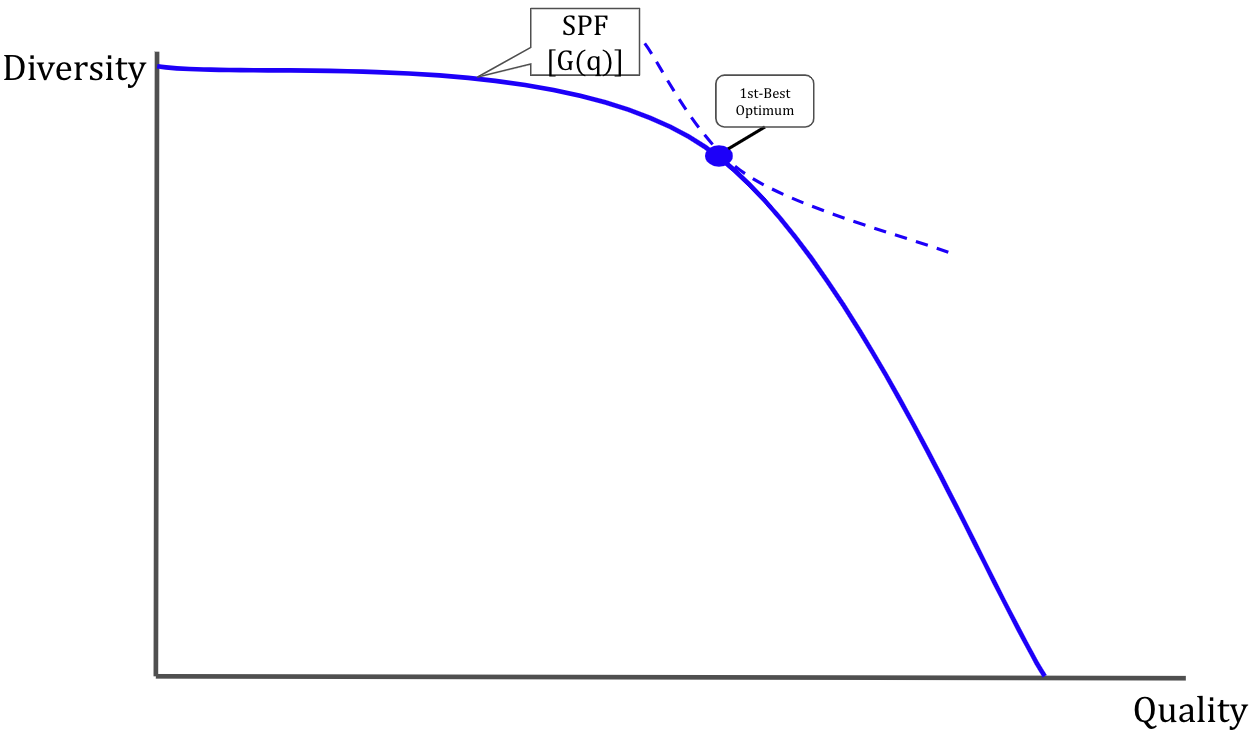
\includegraphics[width=1\textwidth,height=\textheight,keepaspectratio]{\figurepath/model_spf.png} 
        \begin{notes}
    This figure depicts an example solution to an iteration of the selection problem with no computational costs, which is described in Equation \ref{eq:selection_simple}. The solid blue curve represents the selection possibilities frontier (SPF), the dotted blue curve represents the organizations indifference curve corresponding to the highest achievable utility, and the blue dot represents the diversity and performance of the optimal choice (i.e. the first-best solution). 
        \end{notes}
    \end{figure}
    
    \newpage
    \begin{figure}[!htb]
    \centering
        \caption{The Selection Problem With Complexity}\label{fig:model_complex}
      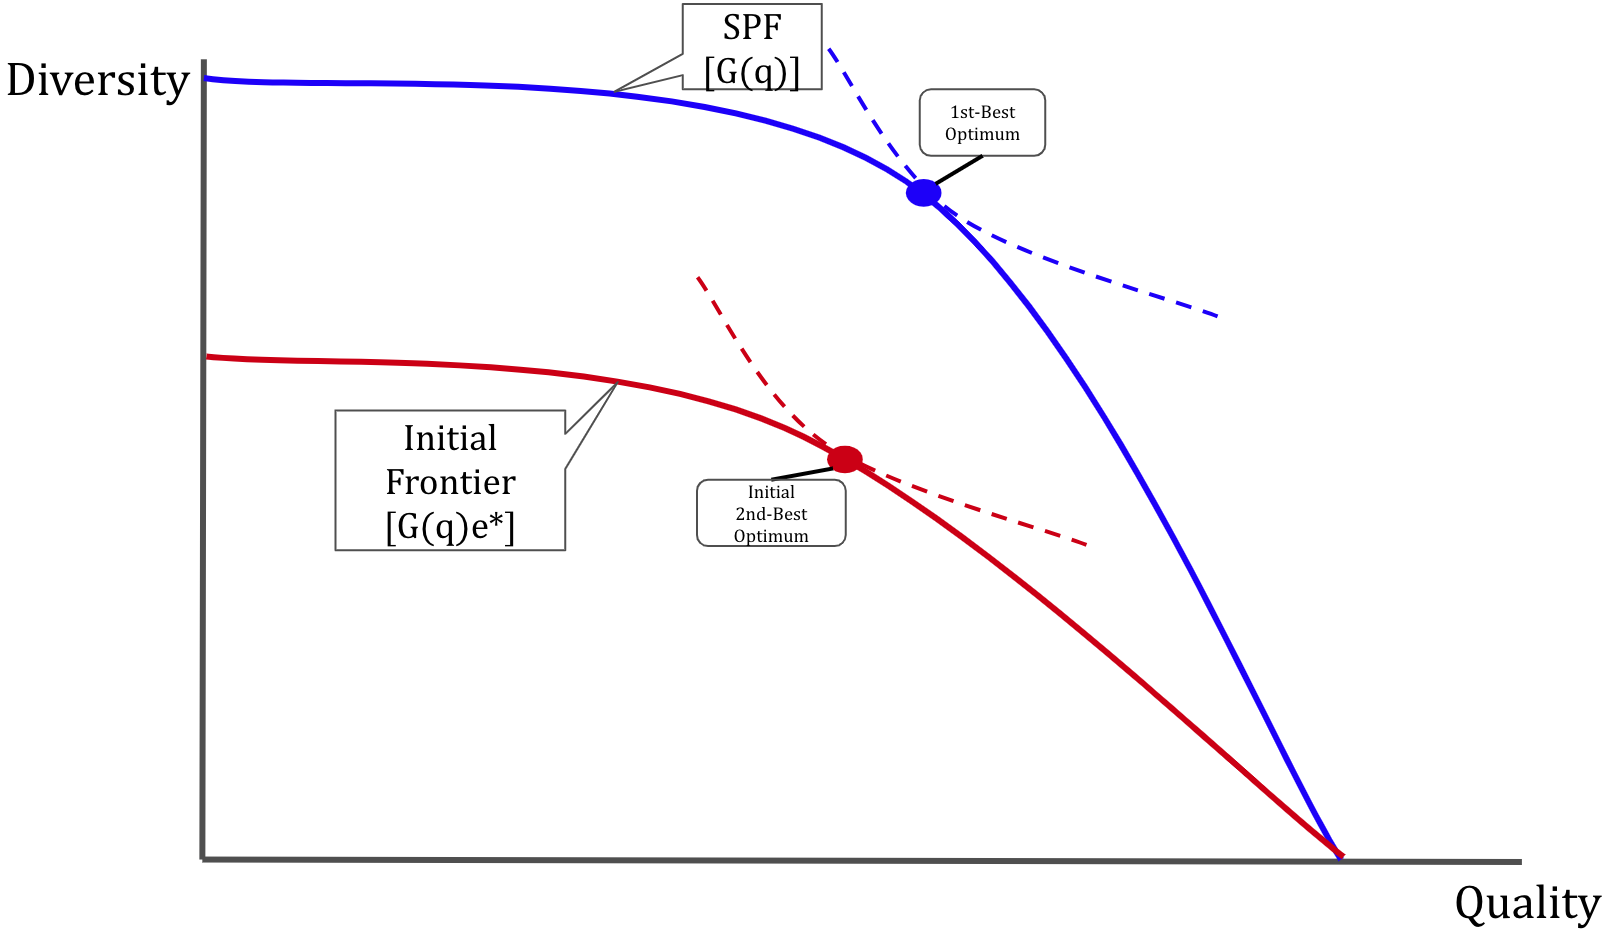
\includegraphics[width=1\textwidth,height=\textheight,keepaspectratio]{\figurepath/model_complex.png} 
        \begin{notes}
    This figure depicts an example solution to an iteration of the selection problem with complexity induced search costs, which is described in Equation \ref{eq:objective}. As in Figure \ref{fig:model_spf}, the solid blue curve represents the SPF, the dotted blue curve represents the organization's indifference curve corresponding to the highest achievable utility without search costs, and the blue dot represents the diversity and performance of the first-best solution. Additionally, the solid red curve represents the accessible frontier with optimal search, the dotted red curve that represents the highest achievable utility with search costs, and the red dot that represents the diversity and performance of the optimal cohort with search costs (i.e. the second-best solution).
        \end{notes}
    \end{figure}
    
    \newpage
    \begin{figure}[!htb]
    \centering
        \caption{The Selection Problem With Complexity and Access to the SPF}\label{fig:model_spf_est}
      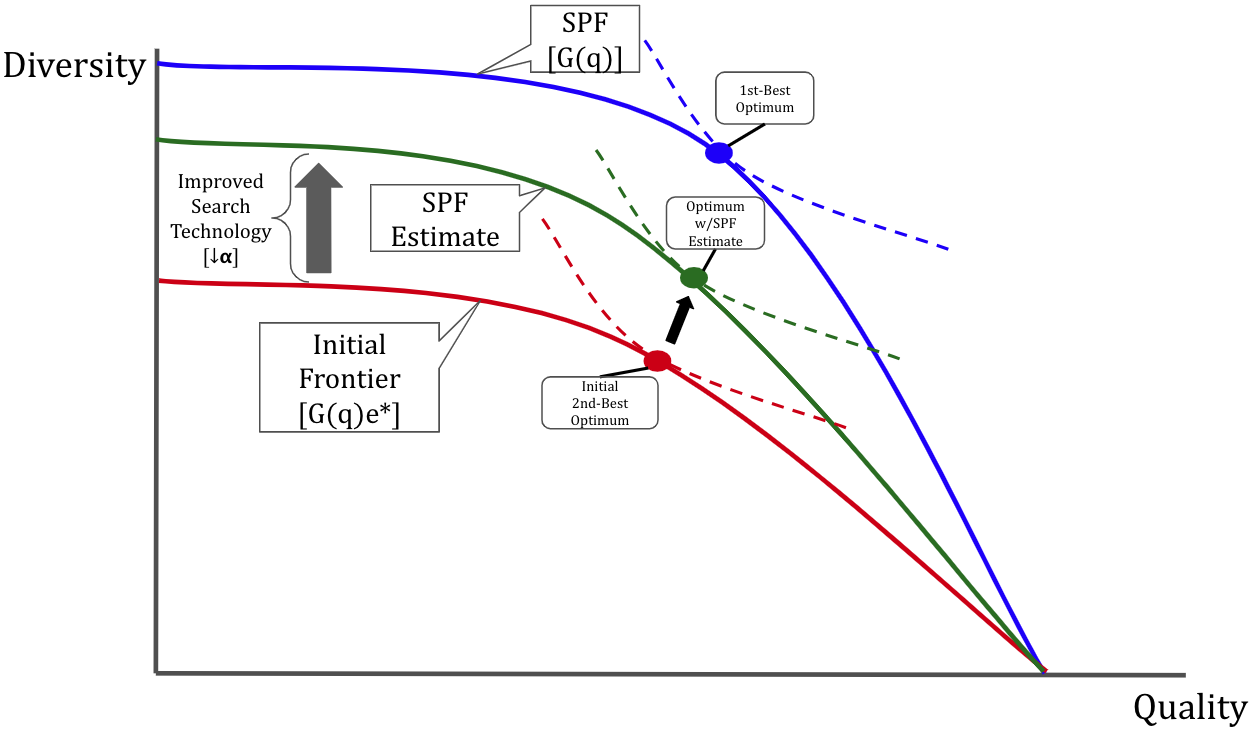
\includegraphics[width=1\textwidth,height=\textheight,keepaspectratio]{\figurepath/model_spf_est.png} 
        \begin{notes}
    This figure depicts an example solution to an iteration of the selection problem with complexity induced search costs, which is described in Equation \ref{eq:objective}. As in Figure \ref{fig:model_spf}, the solid blue curve represents the SPF, the dotted blue curve represents the organization's indifference curve corresponding to the highest achievable utility without search costs, and the blue dot represents the diversity and performance of the first-best solution. And, as in \ref{fig:model_spf}, the solid red curve represents the accessible frontier with optimal search, the dotted red curve that represents the highest achievable utility with search costs, and the red dot that represents the diversity and performance of the second-best cohort with poor search technology (i.e. high $\alpha$). And, the green curves and dot represent the SPF estimate that is accessible with an improved search technology and new second-best solution, respectively. The difference between the initial second-best solution and the new solution is a graphical representation of the implications of the comparative static signed in Equation \ref{eq:comp_stat} ($\frac{\partial e^*}{\partial \alpha}$).
        \end{notes}
    \end{figure}
    
    
    \newpage
    \null %The \null -> \vfill -> figure code -> \vfill code centers the figure vertically on the page
    \vfill
    \begin{center}
    \begin{figure}[!htb]
    \centering
        \caption{Program Selection Design}\label{fig:design}
      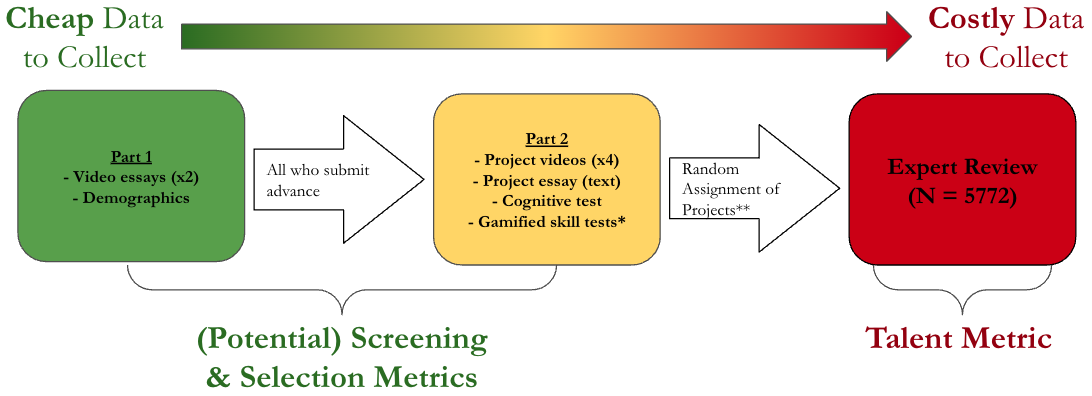
\includegraphics[width=\textwidth,height=\textheight,keepaspectratio]{results/figures/selection_design_schematic.png} 
        \begin{notes}
        This figure schematizes the key elements of the talent investment program's data collection and selection process. 
        \end{notes}
    \end{figure}
    \end{center}
    \vfill
    
    
    \newpage
    \begin{landscape}
    \begin{figure}[!htb]
    \centering
        \caption{Distribution of Applicant Countries (Top 5 Labeled) }\label{fig:country_dist_all}
      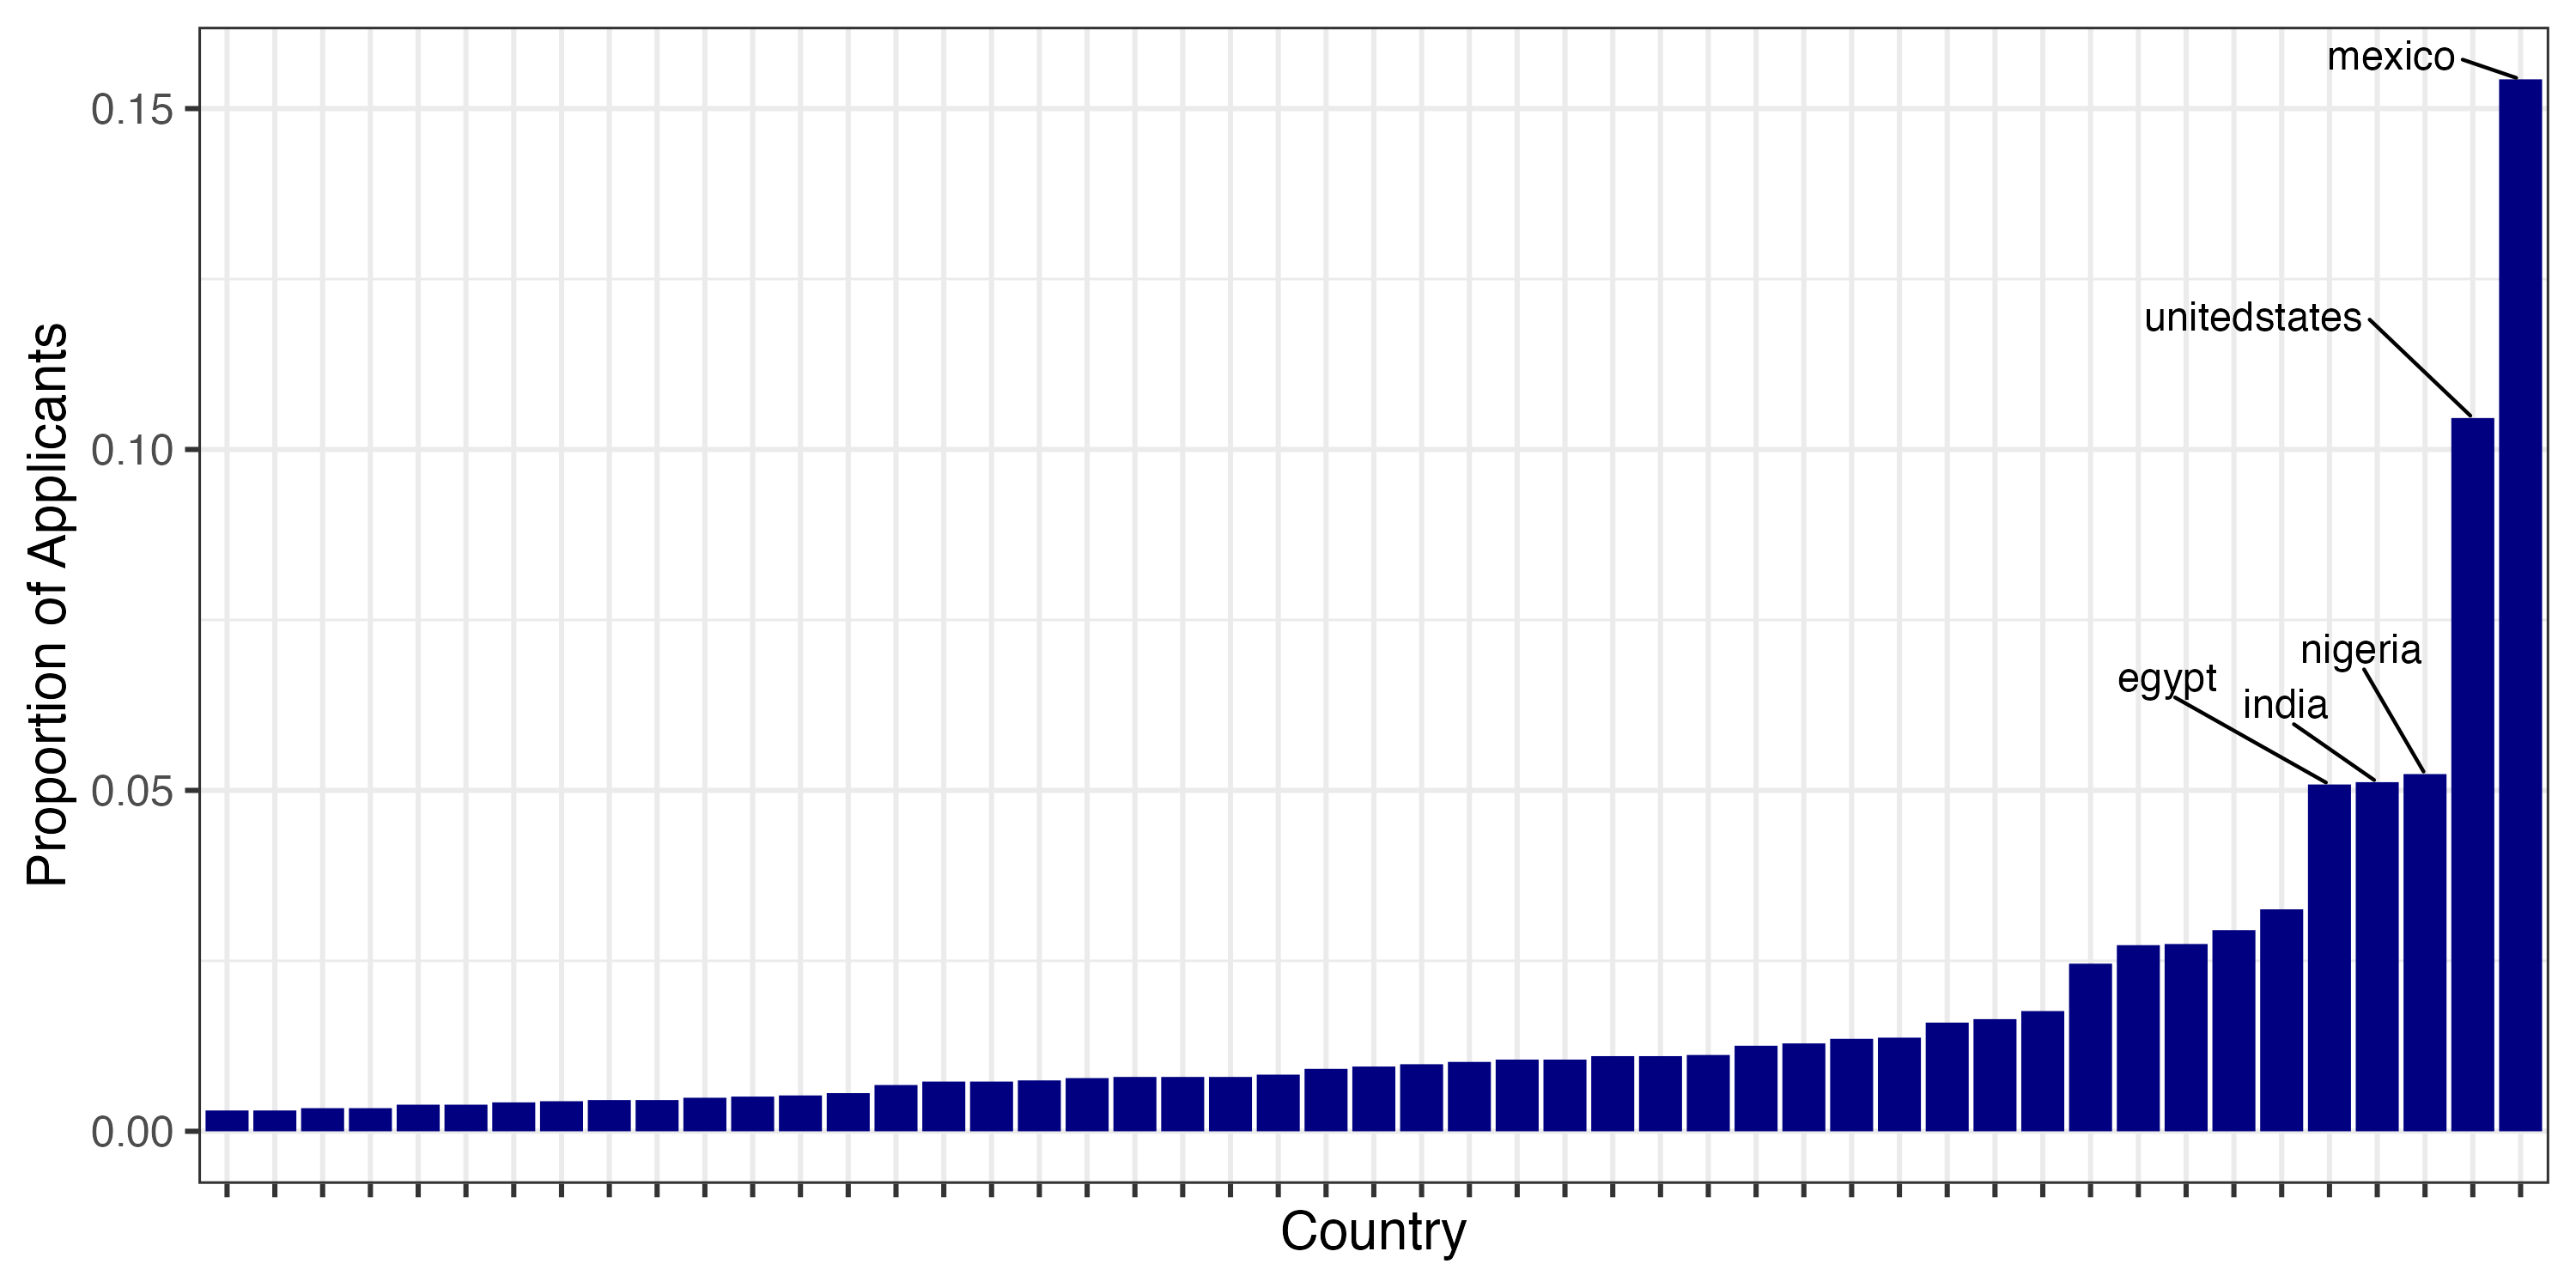
\includegraphics[width=1.3\textwidth,height=\textheight,keepaspectratio]{\figurepath/candidate_countries.png} 
        \begin{notes}
        Data come from surveys completed by applicants. Data are pooled across all three application cohorts. Overall applicants come from 153 different countries. The distribution of proportions of applicants by country in this figure are limited to the 50 countries from which there were the most applicants. The top 5 countries are labeled on the figure. 
        \end{notes}
    \end{figure}
    \end{landscape}
    
    
    \begin{figure}[!htb]
        \centering
        \caption{Distributions of Applicant Project Topics and Reviewer Expertise} \label{fig:topic_expertise_dist}
        \begin{subfigure}[t]{\textwidth}
            \centering
                    \caption{Applicant Project Topics} \label{subfig:app_proj_topics}
            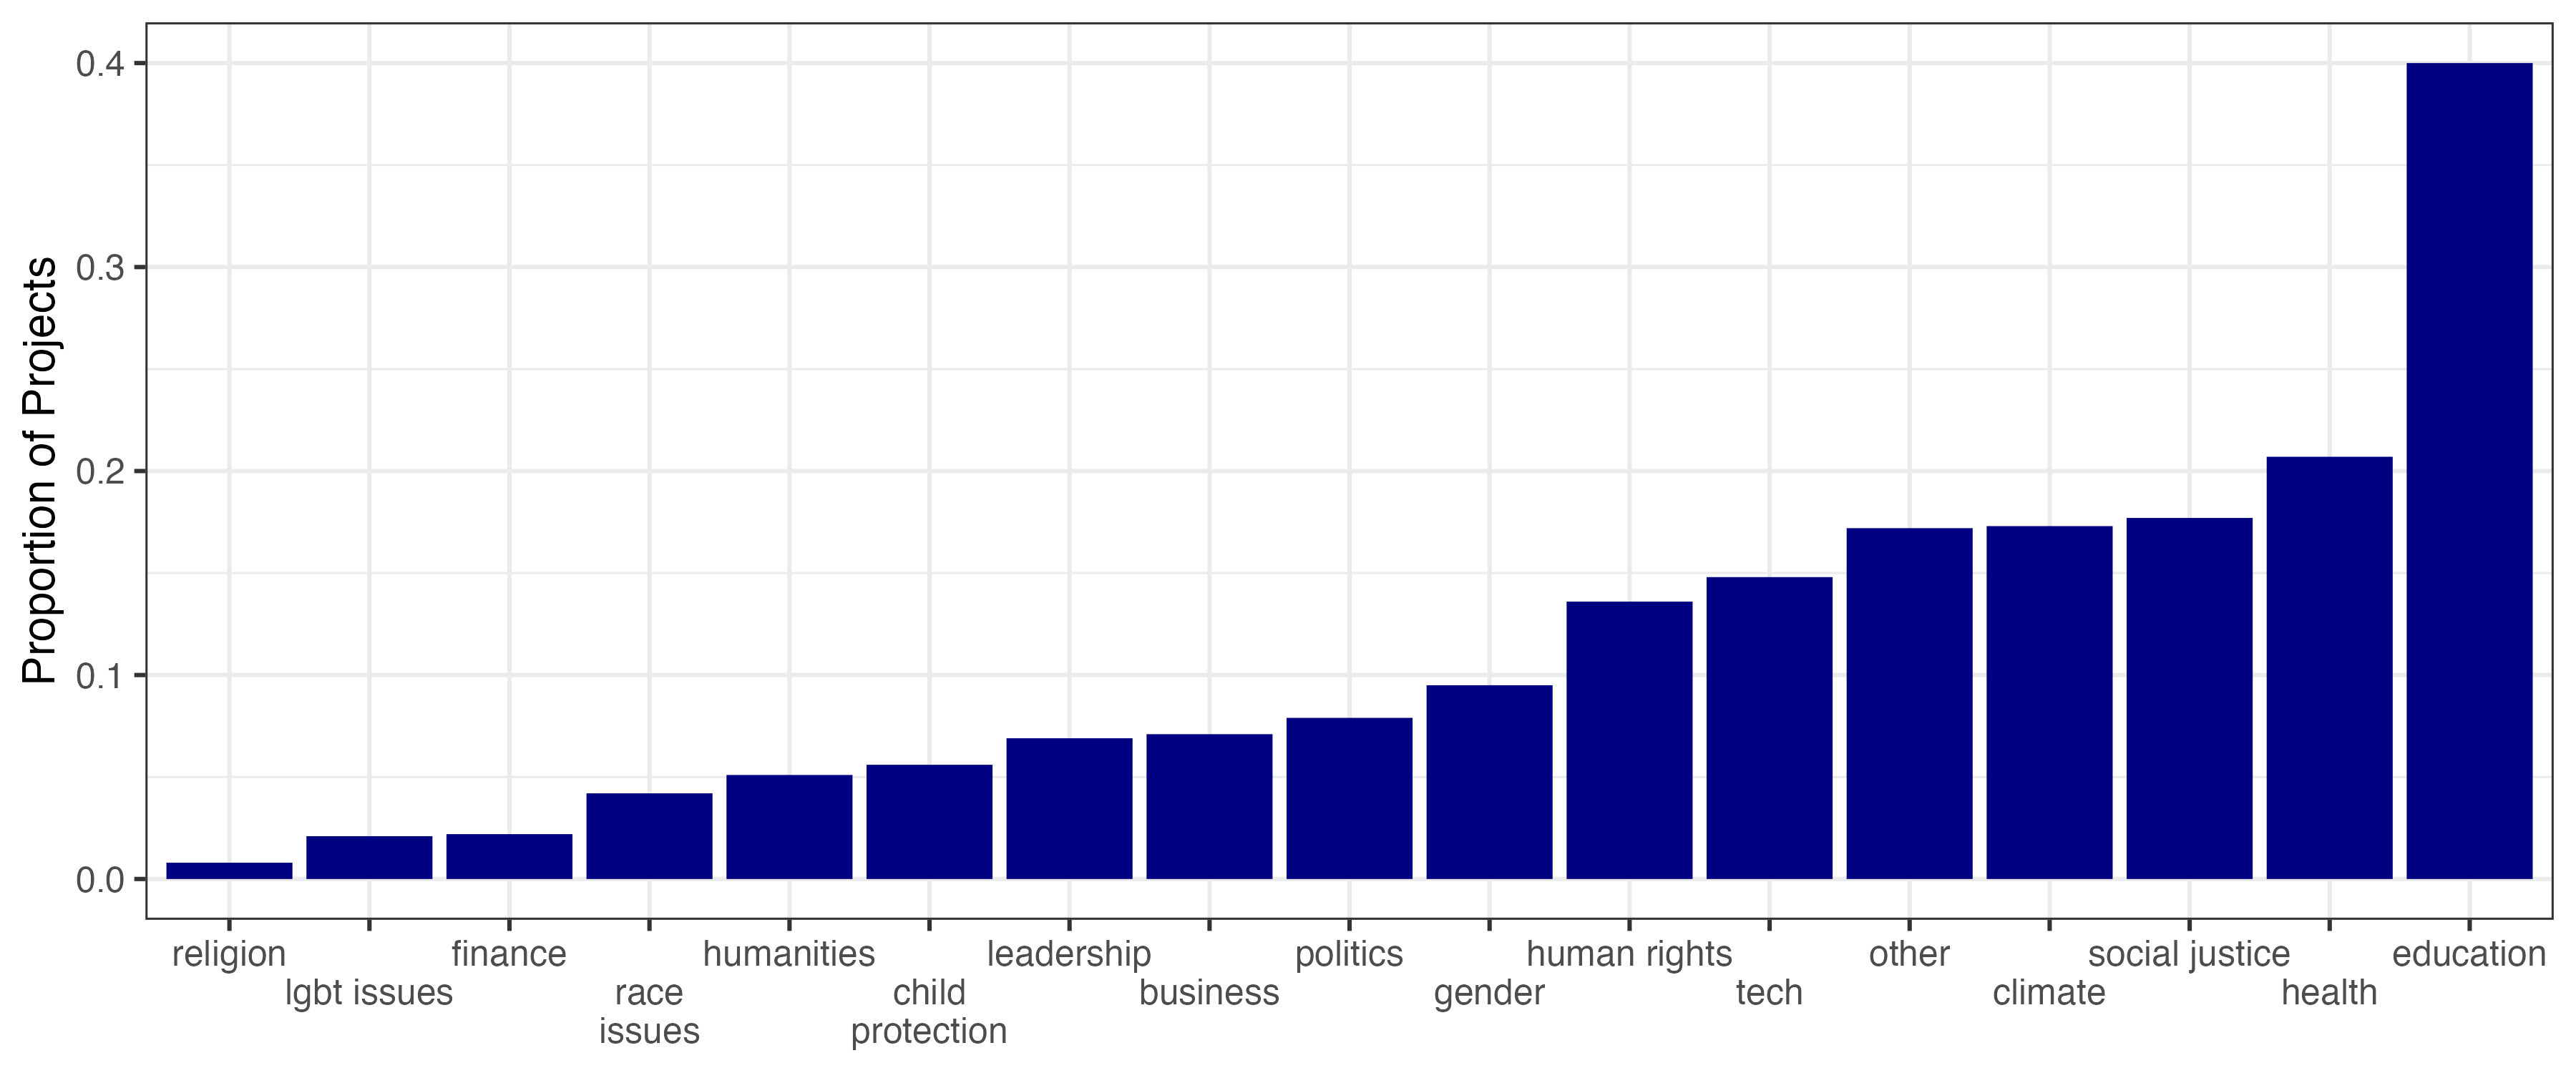
\includegraphics[width=\linewidth]{results/figures/applicant_project_topics.png} 
        \end{subfigure}
        \hfill
        \vspace{1em}
        \begin{subfigure}[t]{\textwidth}
            \centering
                   \caption{Reviewer Areas of Expertise} \label{subfig:rev_expertise}
            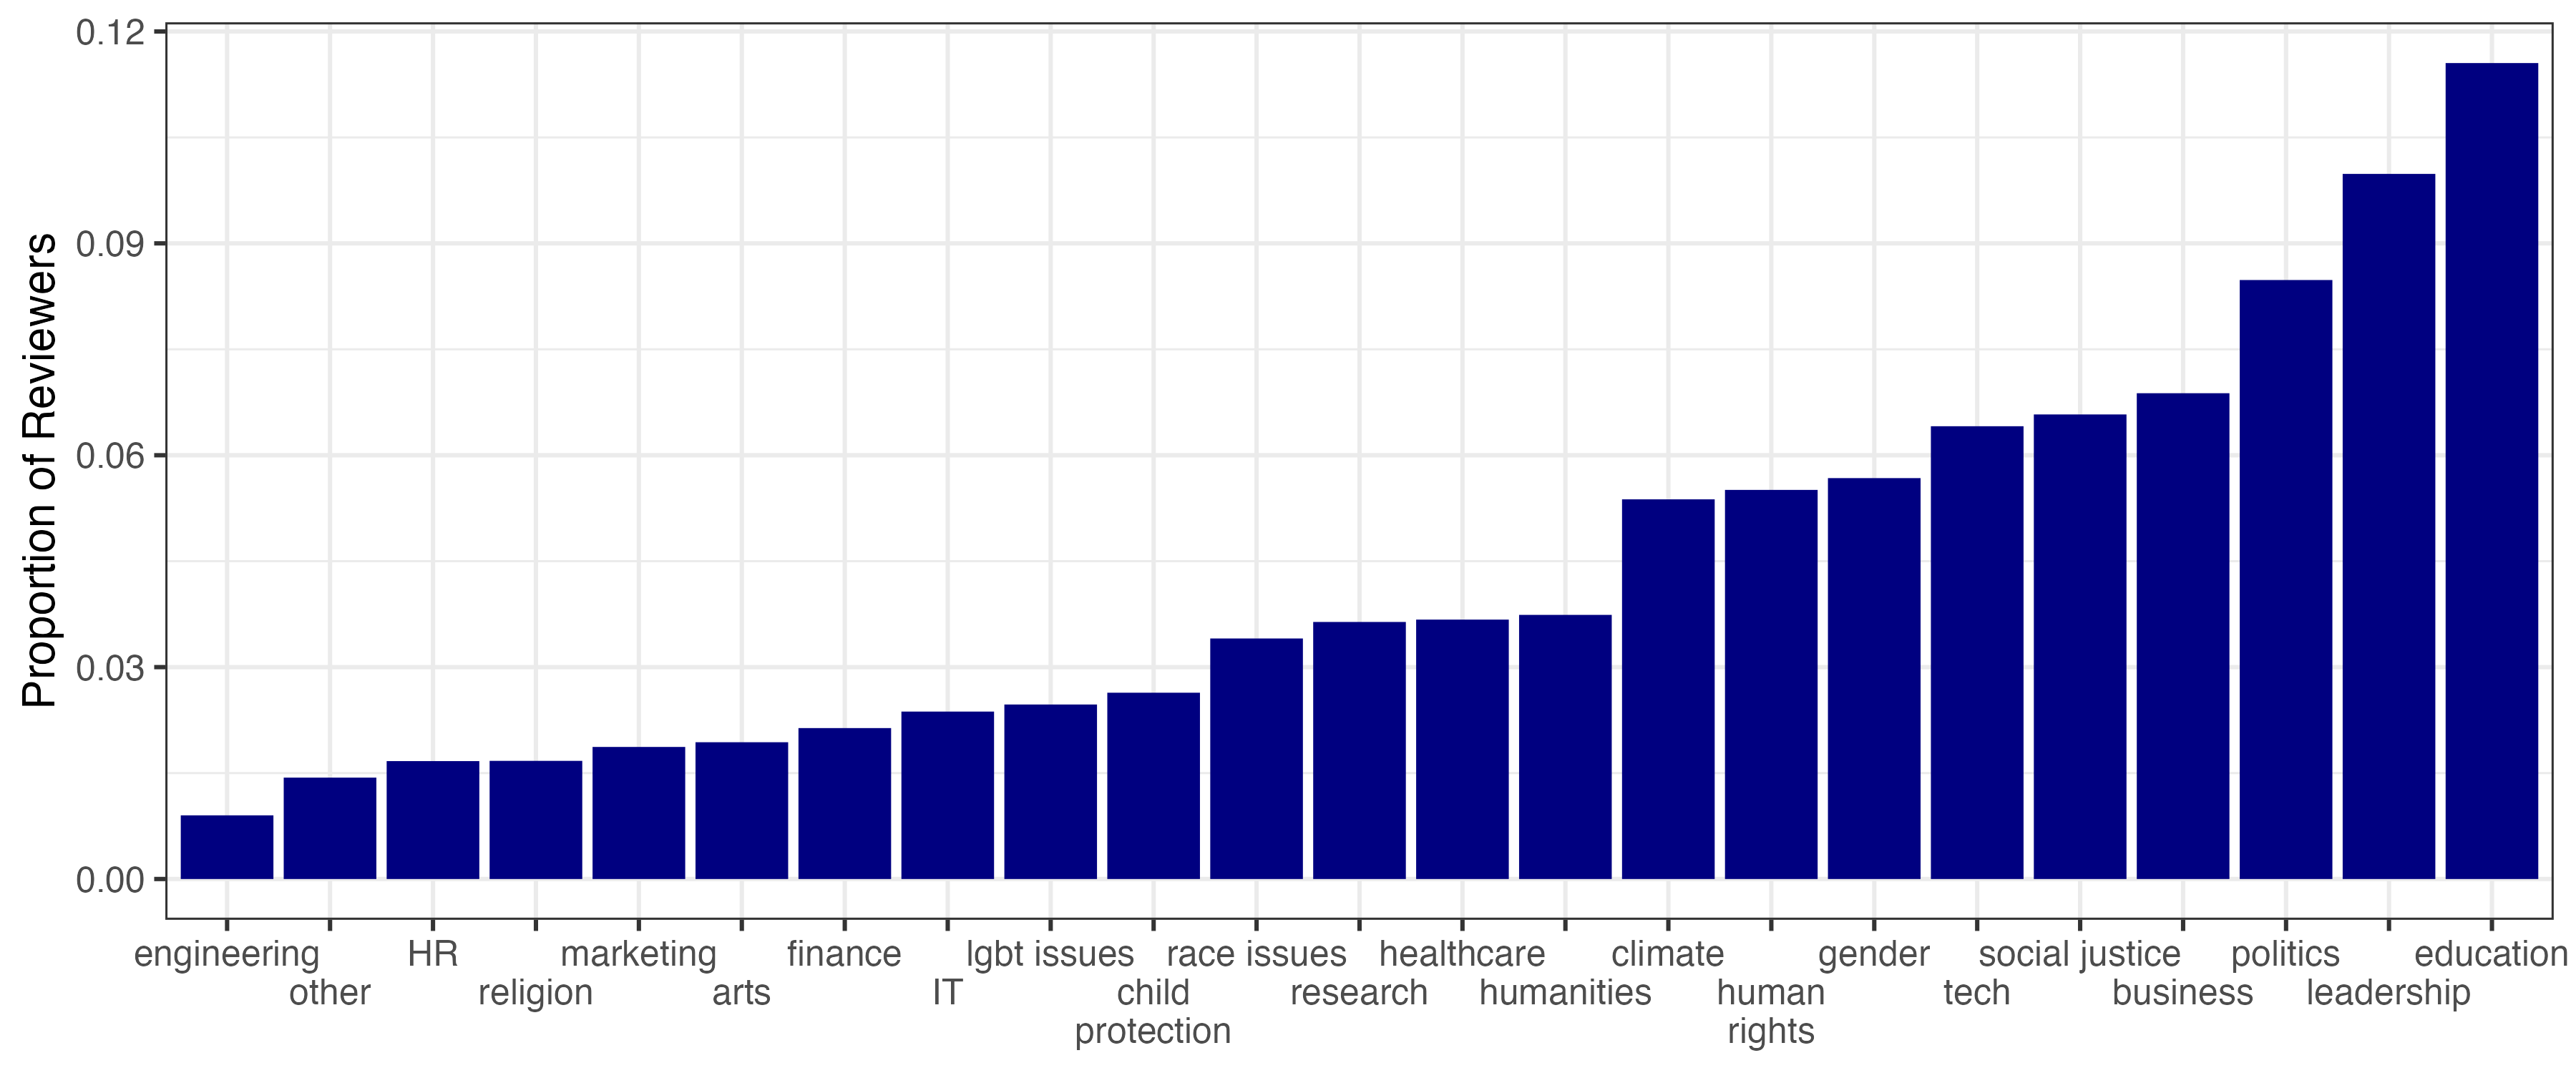
\includegraphics[width=\linewidth]{results/figures/reviewer_expertise.png} 
        \end{subfigure}
        \begin{notes}
        Data come from surveys completed by applicants. Data are pooled across all three application cohorts. Panel (\ref{subfig:app_proj_topics}) depicts the proportion of all applicant projects in each topic category. Panel (\ref{subfig:rev_expertise}) depicts the proportion of project reviewers with each category of expertise.
        \end{notes}
    \end{figure}
    
    
    \begin{figure}[!htb]
        \centering
        \caption{Distributions of Reviewer Industries and Organizations (Cycle 1)}
        \begin{subfigure}[t]{\textwidth}
            \centering
                    \caption{Industries} \label{subfig:rev_industries}
            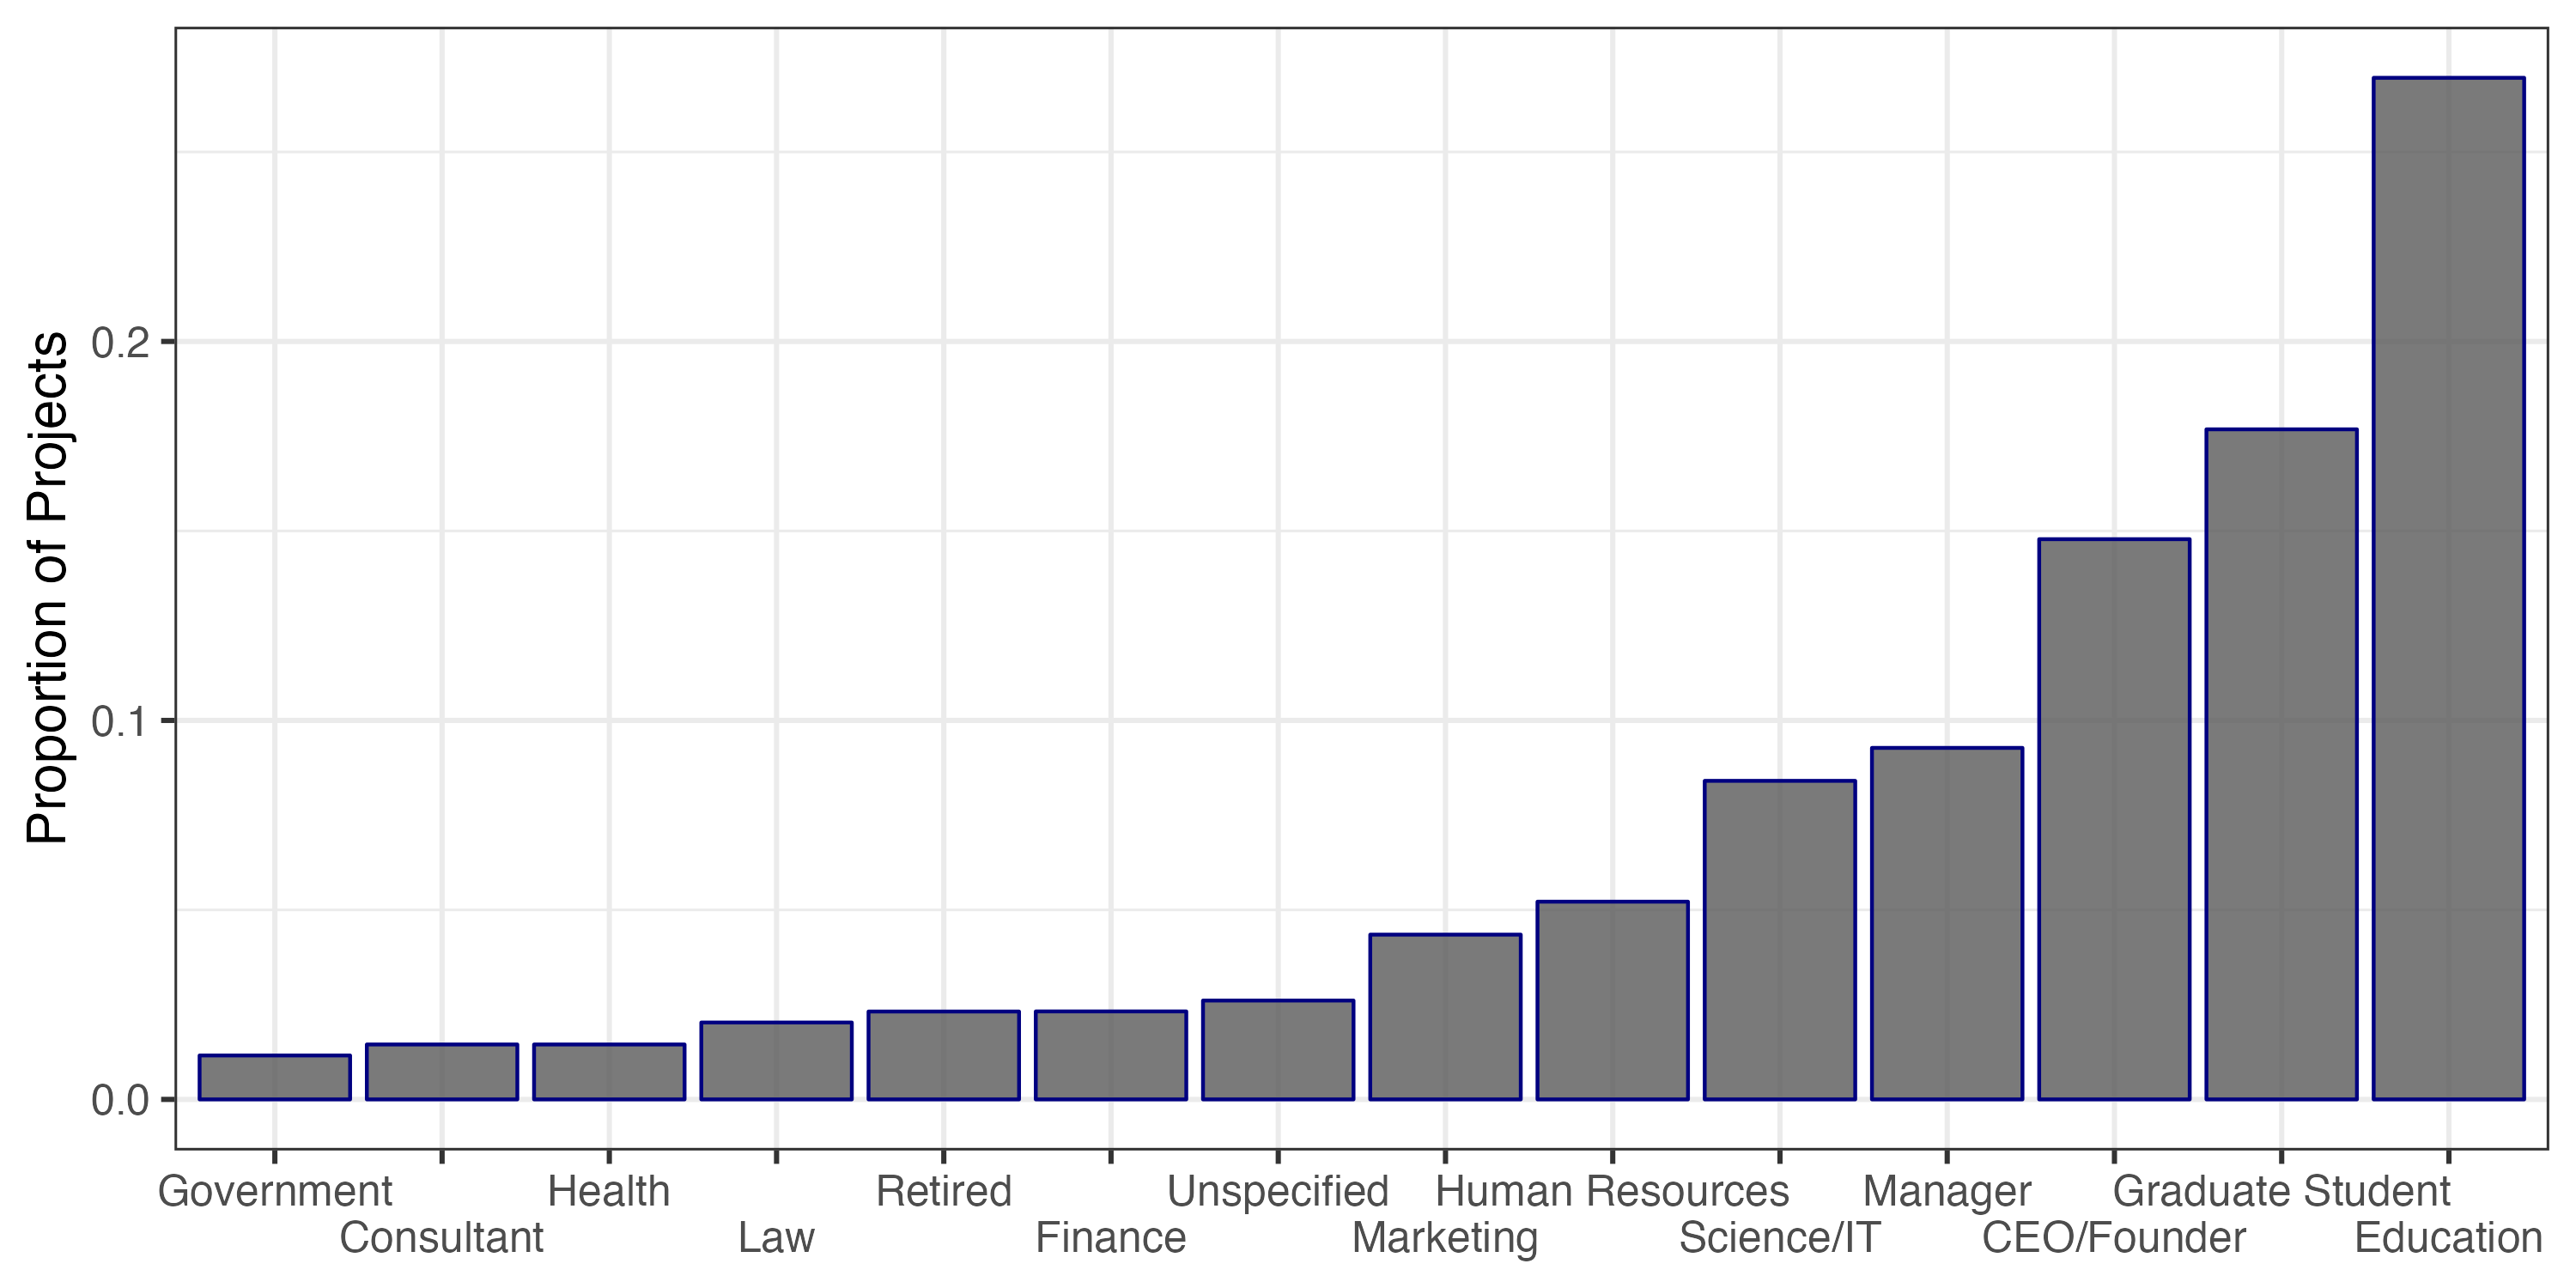
\includegraphics[width=\linewidth]{\figurepath/project_reviewer_industries.png} 
        \end{subfigure}
        \hfill
        \vspace{1em}
        \begin{subfigure}[t]{\textwidth}
            \centering
                   \caption{Organizations (Top 2 Labeled)} \label{subfig:rev_orgs}
            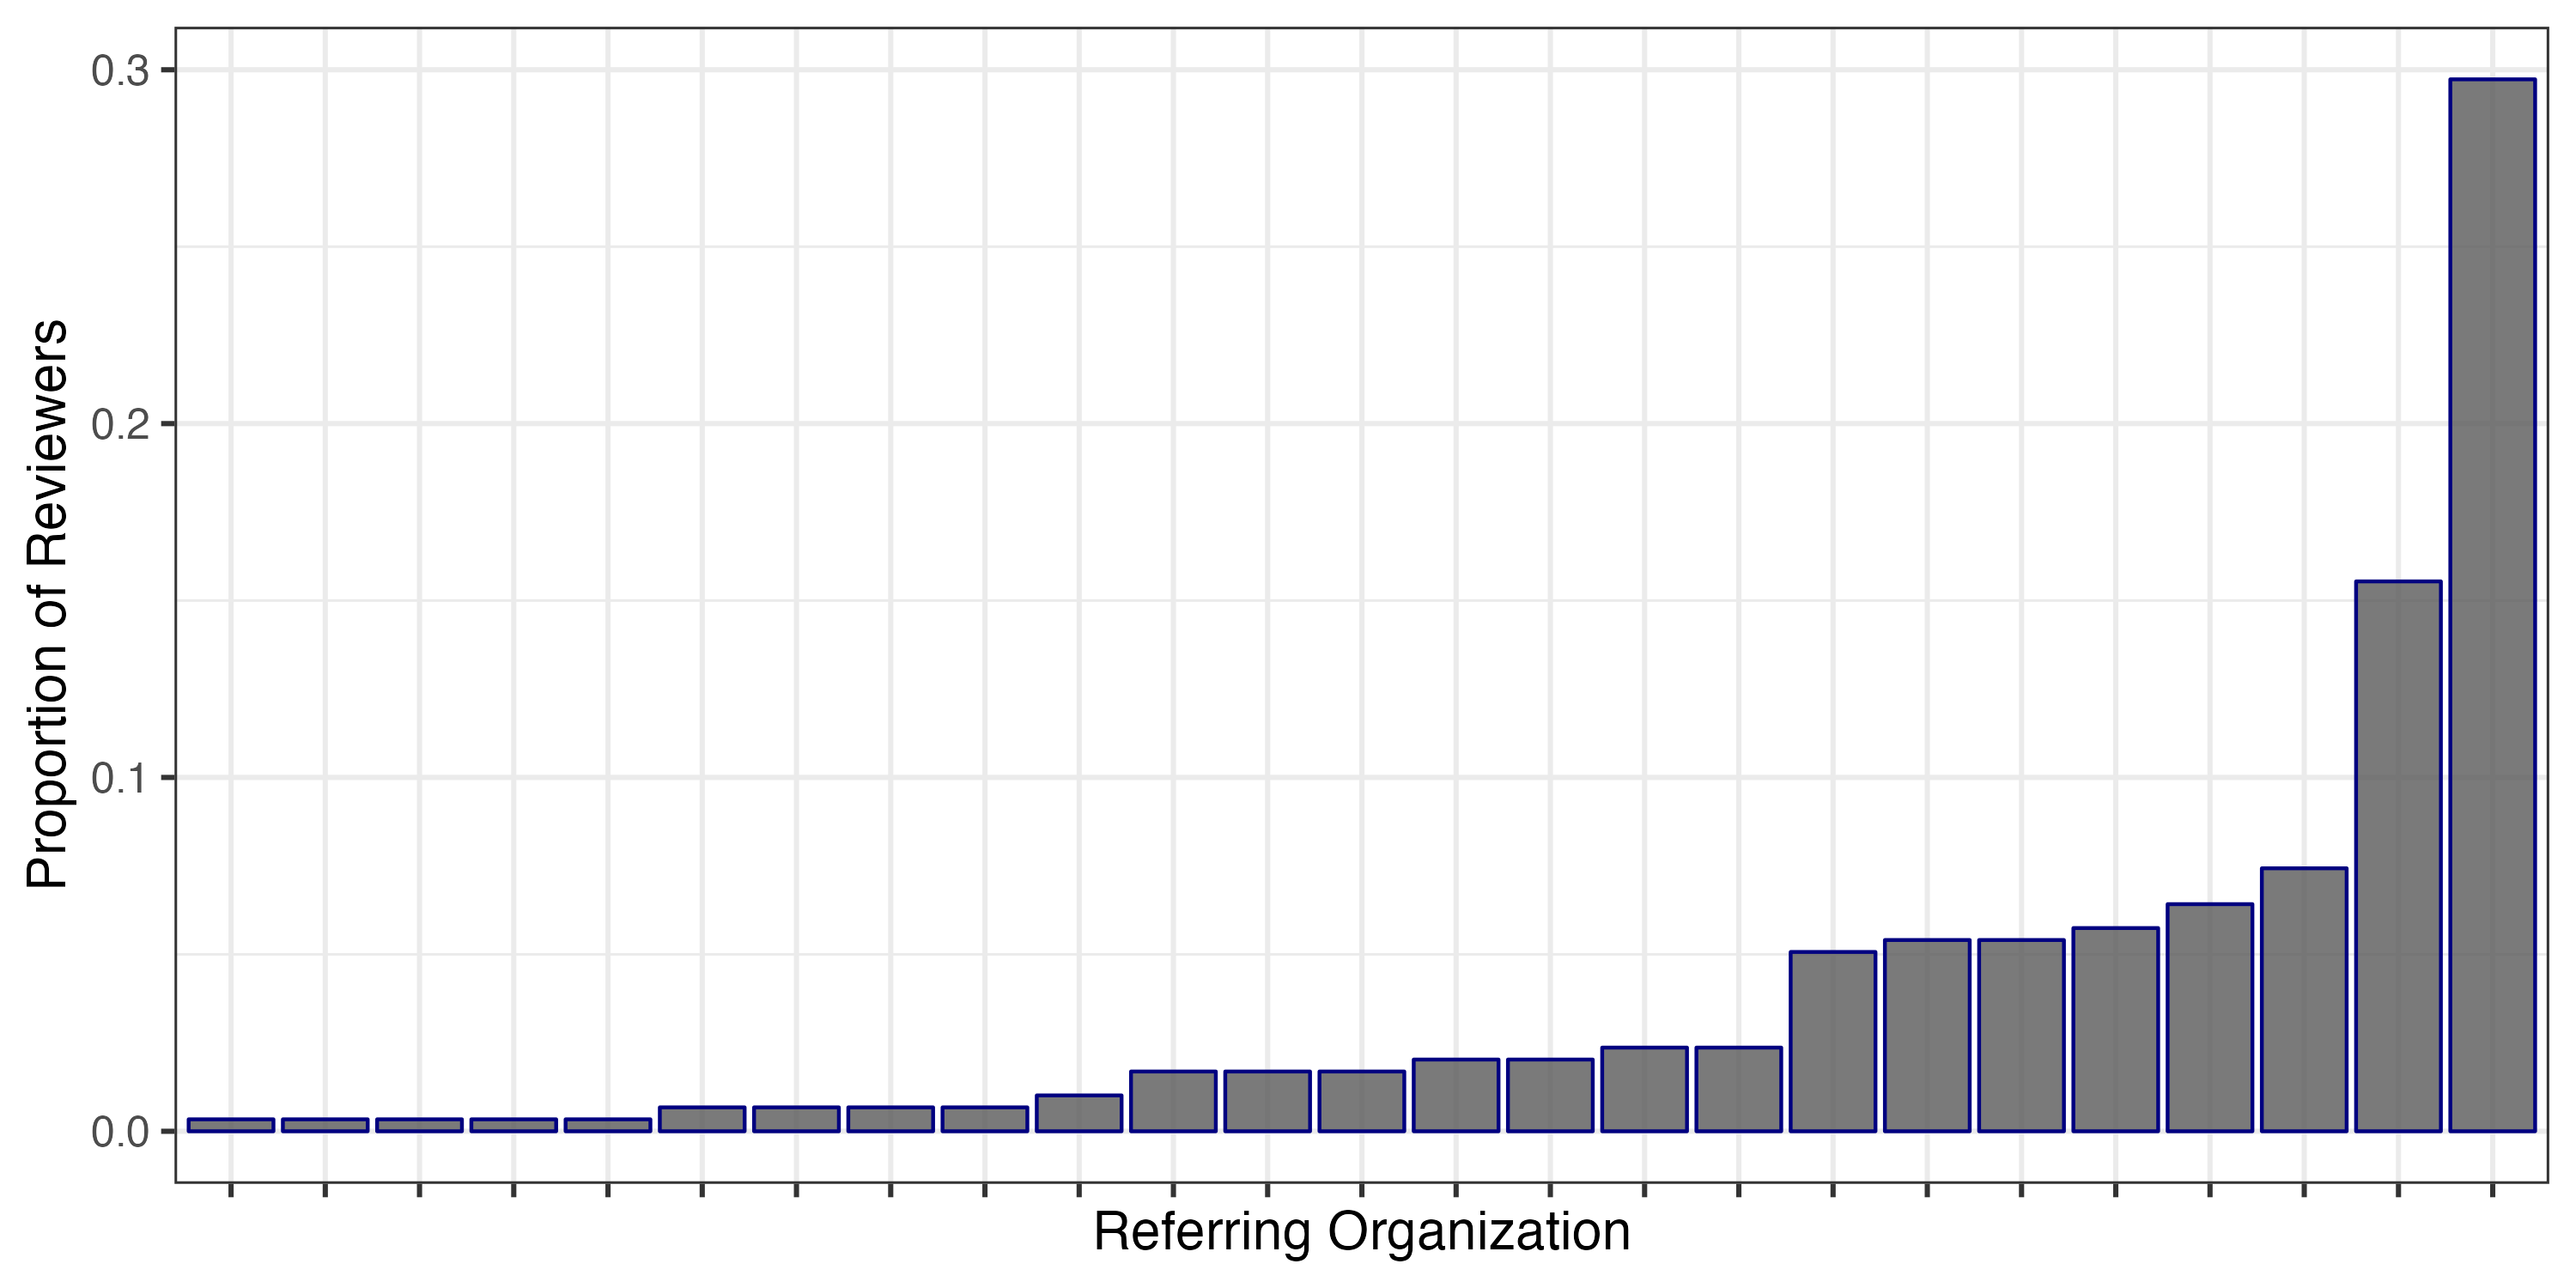
\includegraphics[width=\linewidth]{results/figures/project_reviewer_affiliations.png} 
        \end{subfigure}
        \begin{notes}
        Data come from surveys completed by applicants. Data come from application cycle 1 only (industry and organization information were not collected for the in cycles 2 and 3). Panel (\ref{subfig:rev_industries}) depicts the proportion of all project reviewers by industries. Unfortunately, industries were not categorized using standard codes, but the categories are decipherable. Panel (\ref{subfig:rev_orgs}) depicts the proportion of project reviewers from each organization that referred them. The top two most common referring organizations make up 46\% of all expert reviewers, and the labels on them have been redacted to maintain the program's anonymity. 
        \end{notes}
    \end{figure}
    
    \newpage
    \begin{figure}[!htb]
    \centering
        \caption{Quantifying Cycle 1 Inefficiencies with the SPF} \label{fig:spf_2021}
      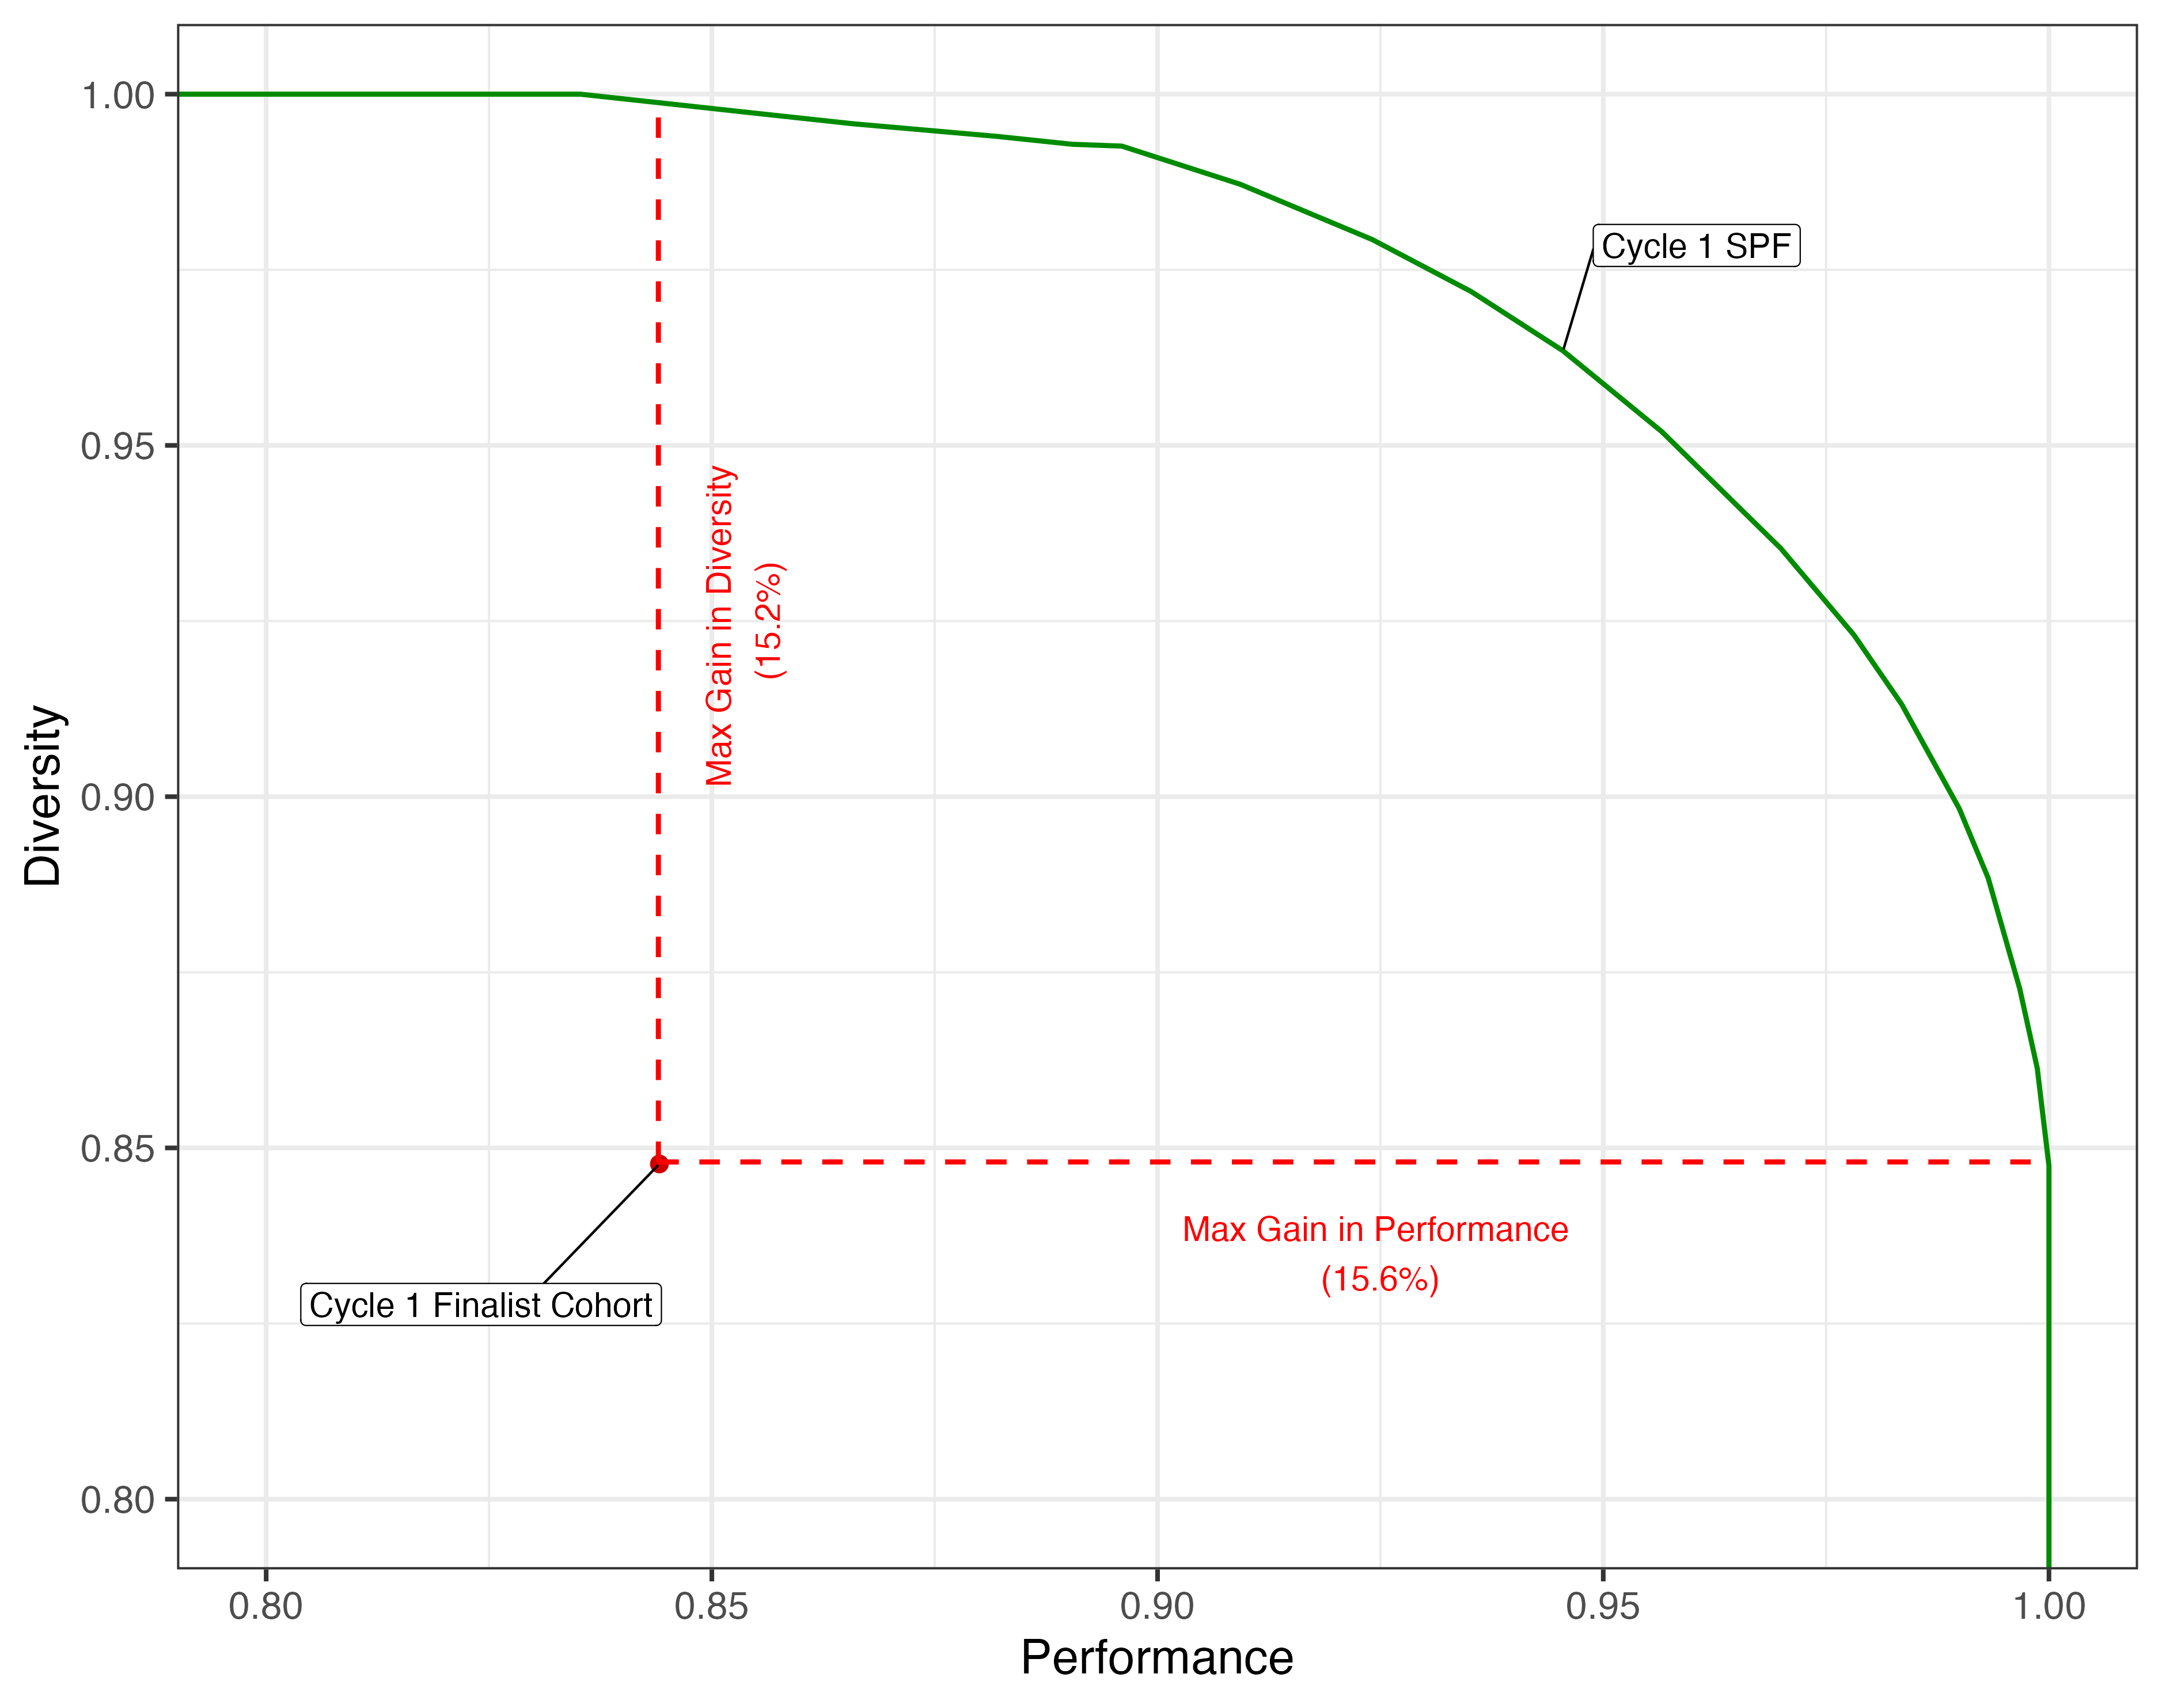
\includegraphics[width=\textwidth,height=\textheight,keepaspectratio]{\figurepath/yr1_spf_finalist.png} 
        \begin{notes}
        This figure displays the SPF we estimate for the cycle 1 finalist cohort. The y-axis represents the diversity score while the x-axis represents average cohort performance (i.e. project scores). The green curve is our estimate of the cycle 1 SPF, which represents the upper bound of diversity that is achievable at every level of cohort performance. The red dot depicts the actual level of diversity and performance of the finalists that were selected in cycle 1. The vertical and horizontal dashed red lines represent the maximum Pareto gain that was possible along the diversity and performance dimensions respectively. In particular, cohort diversity could have been improved by 15.2\% without any reduction in cohort performance. And, cohort performance could have been improved by 15.6\% without any cost to diversity. 
        \end{notes}
    \end{figure}
    
    \newpage
    \begin{figure}[!htb]
    \centering
        \caption{Quantifying Cycle 2 Inefficiencies with the SPF} \label{fig:spf_2022}
      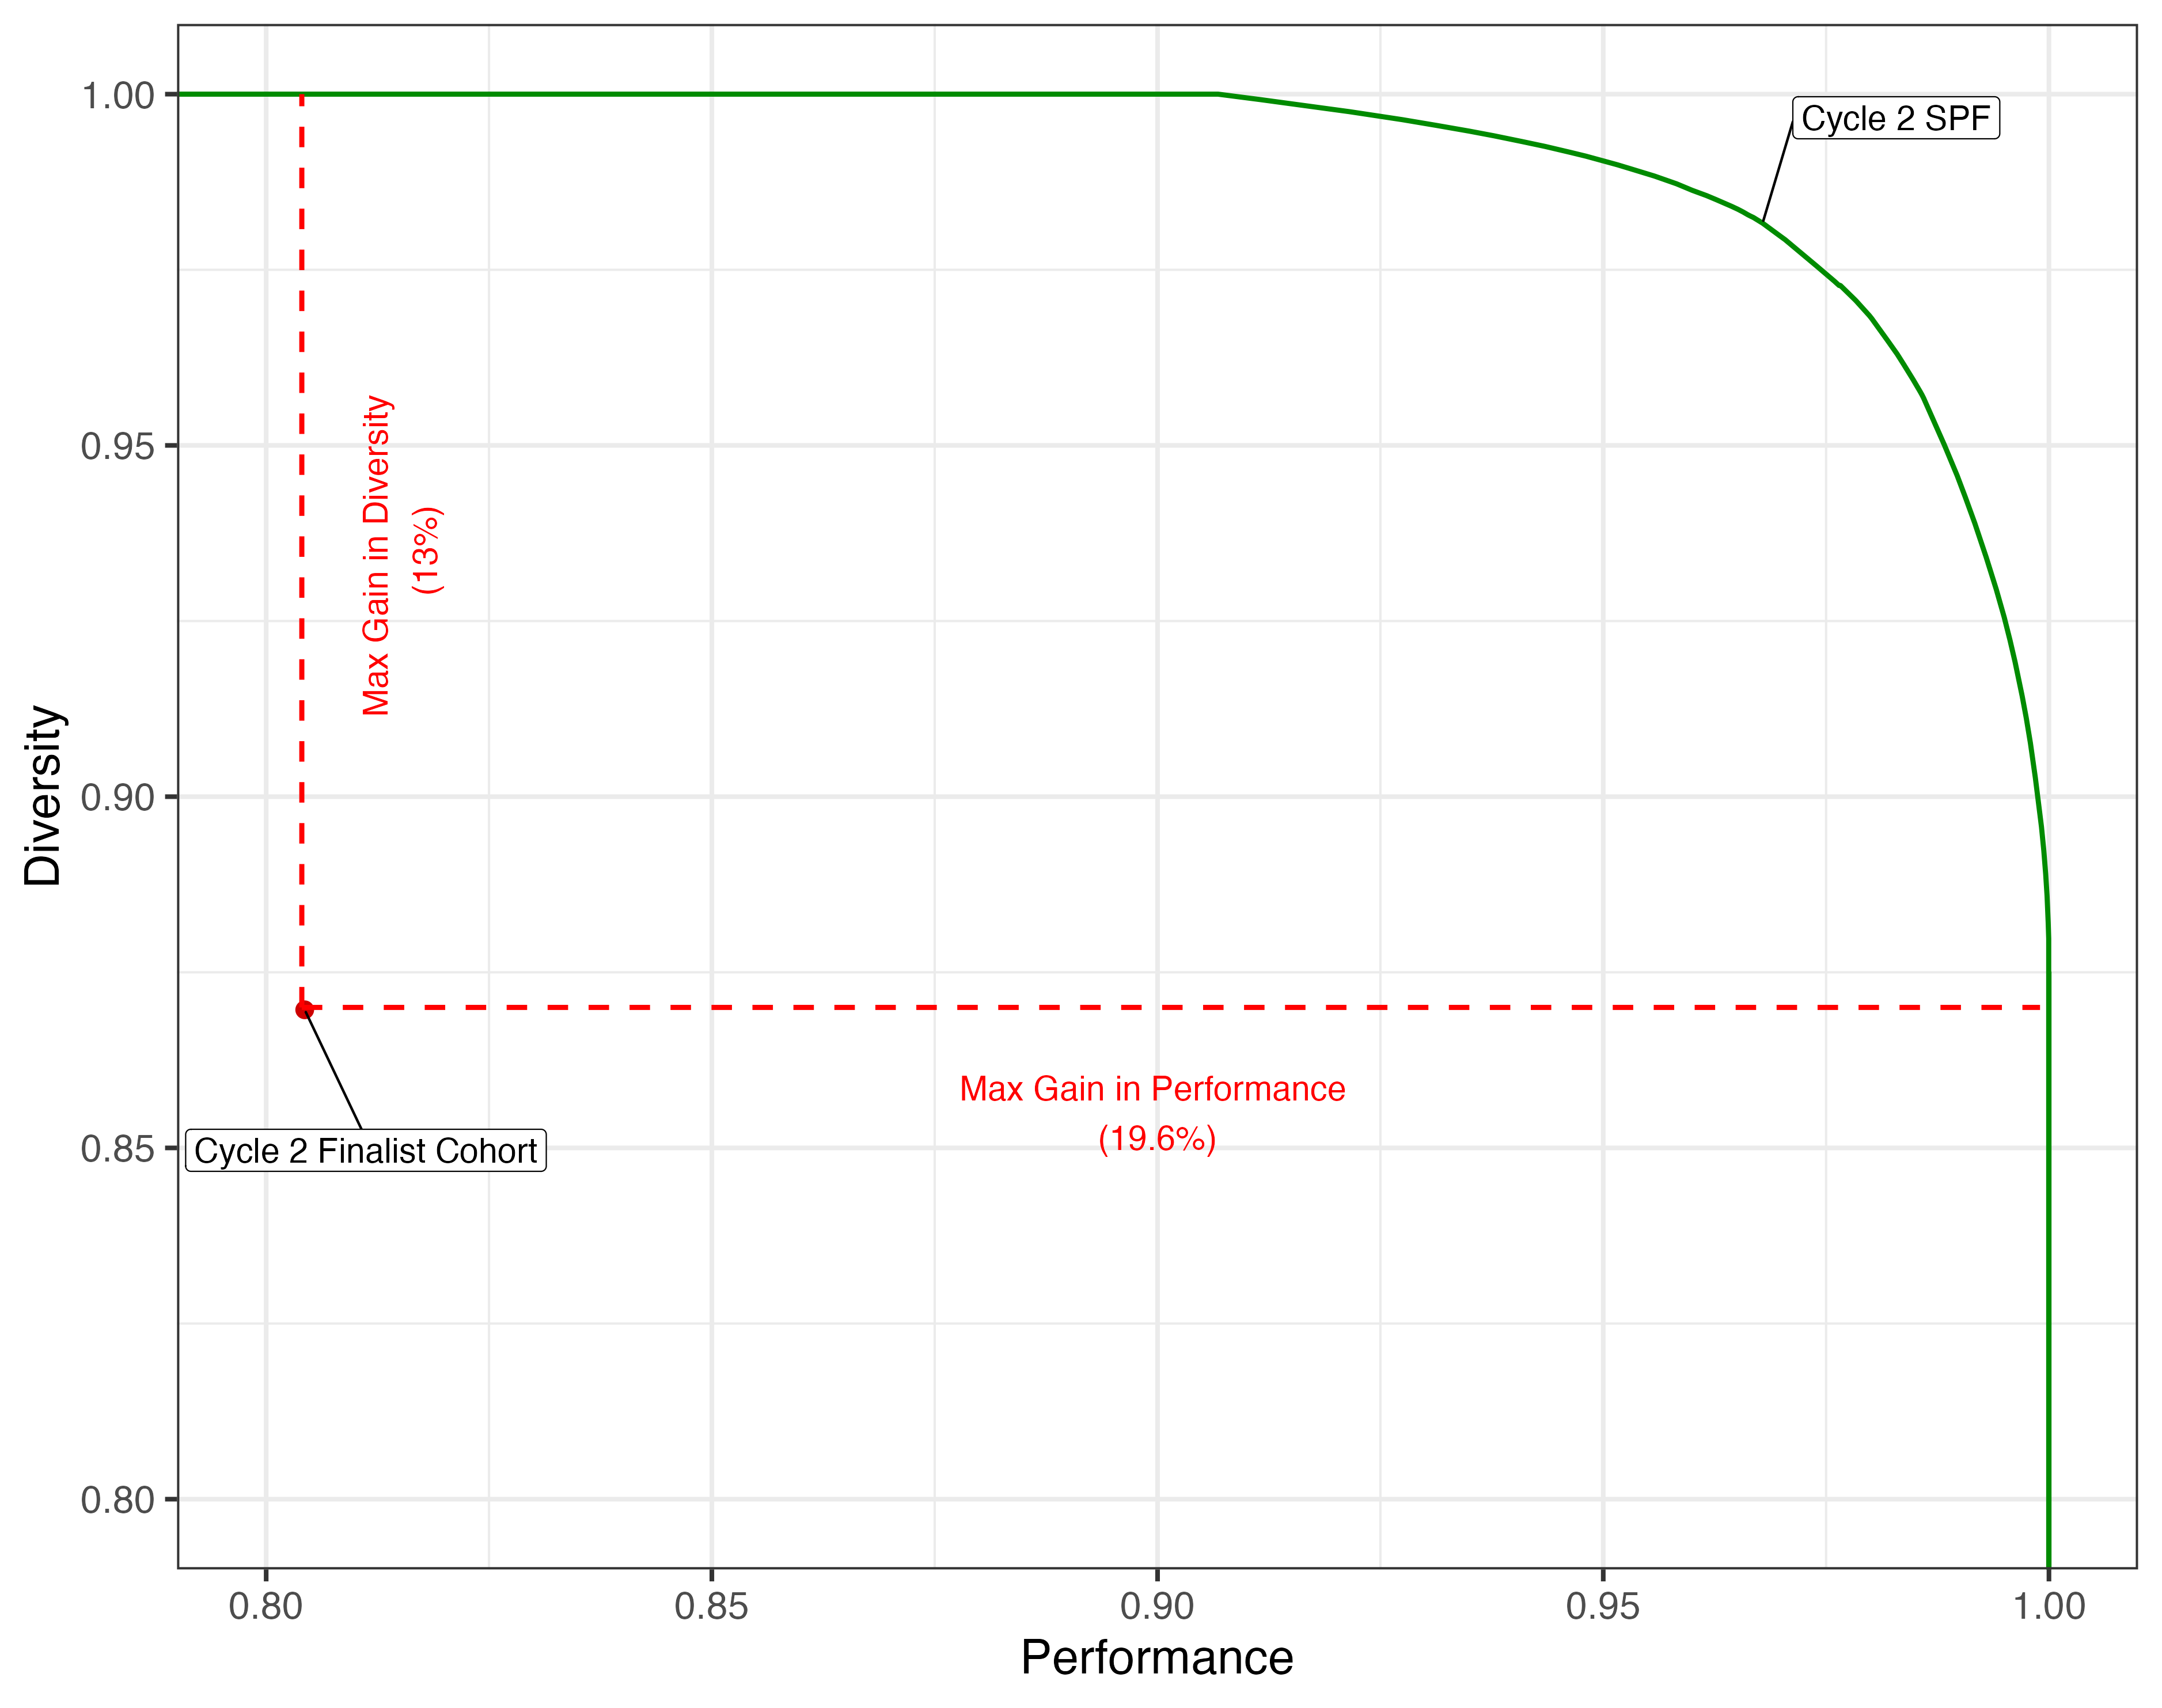
\includegraphics[width=\textwidth,height=\textheight,keepaspectratio]{\figurepath/yr2_spf_finalist.png} 
        \begin{notes}
        This figure displays the SPF we estimate for the cycle 2 finalist cohort. The y-axis represents the diversity score while the x-axis represents average cohort performance (i.e. project scores). The green curve is our estimate of the cycle SPF, which represents the upper bound of diversity that is achievable at every level of cohort performance. The red dot depicts the actual level of diversity and performance of the finalists that were selected in cycle 2. The vertical and horizontal dashed red lines represent the maximum Pareto gain that was possible along the diversity and performance dimensions respectively. In particular, cohort diversity could have been improved by 13\% without any reduction in cohort performance. And, cohort performance could have been improved by 19.6\% without any cost to diversity. 
        \end{notes}
    \end{figure}
    
    \newpage
    \begin{figure}[!htb]
    \centering
        \caption{Quantifying Cycle 3 Efficiency Gains with the SPF} \label{fig:spf_2023}
      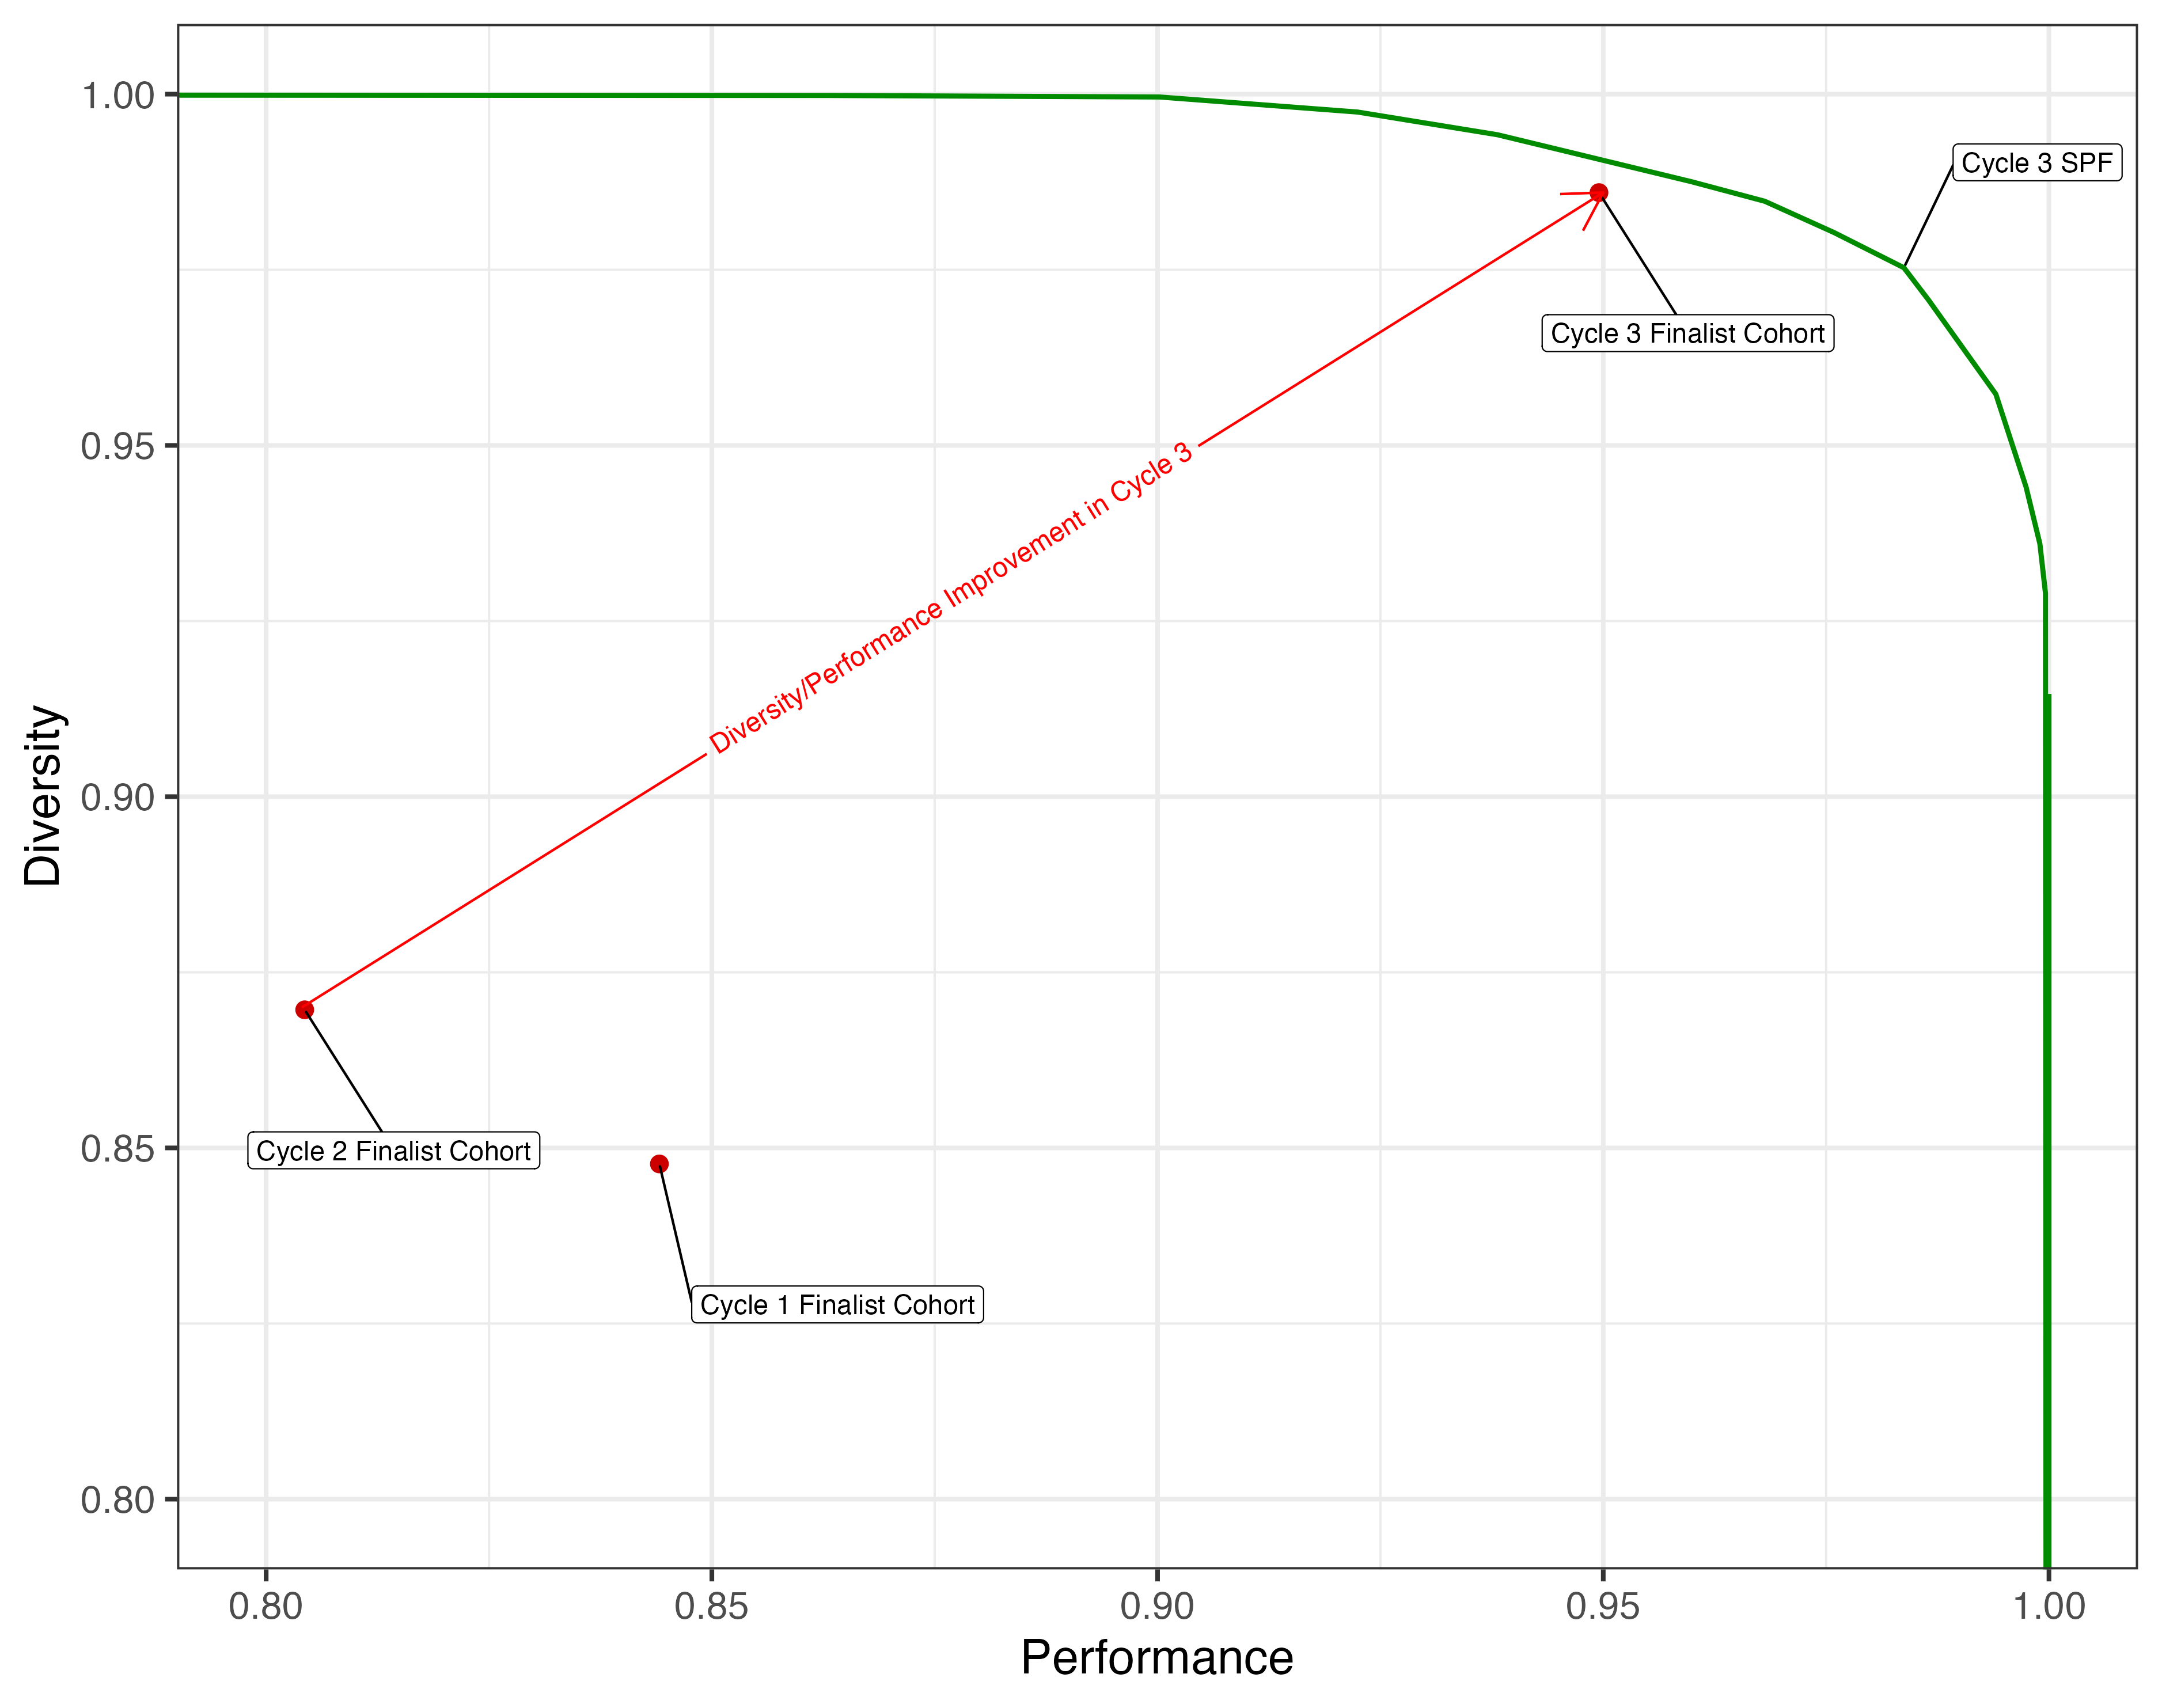
\includegraphics[width=\textwidth,height=\textheight,keepaspectratio]{\figurepath/yr3_spf_finalist.png} 
        \begin{notes}
        This figure displays the SPF we estimate for the cycle 3 finalist cohort. The y-axis represents the diversity score while the x-axis represents average cohort performance (i.e. project scores). The green curve is our estimate of the cycle 3 SPF, which represents the upper bound of diversity that is achievable at every level of cohort performance.The red dots depict the actual level of diversity and performance of the finalists that were selected in cycles 1-3, respectively. The diagonal dashed red line represents the distance in diversity-performance space between the cycle 2 cohort and the cycle 3 cohort. In cycle 3, there are no significant Pareto improvements on either diversity or performance. 
        \end{notes}
    \end{figure}
    
    
    \newpage
    \begin{figure}[!htb]
    \centering
        \caption{Permutation Tests of Significance of Inefficiencies} \label{fig:permutation_tests}
      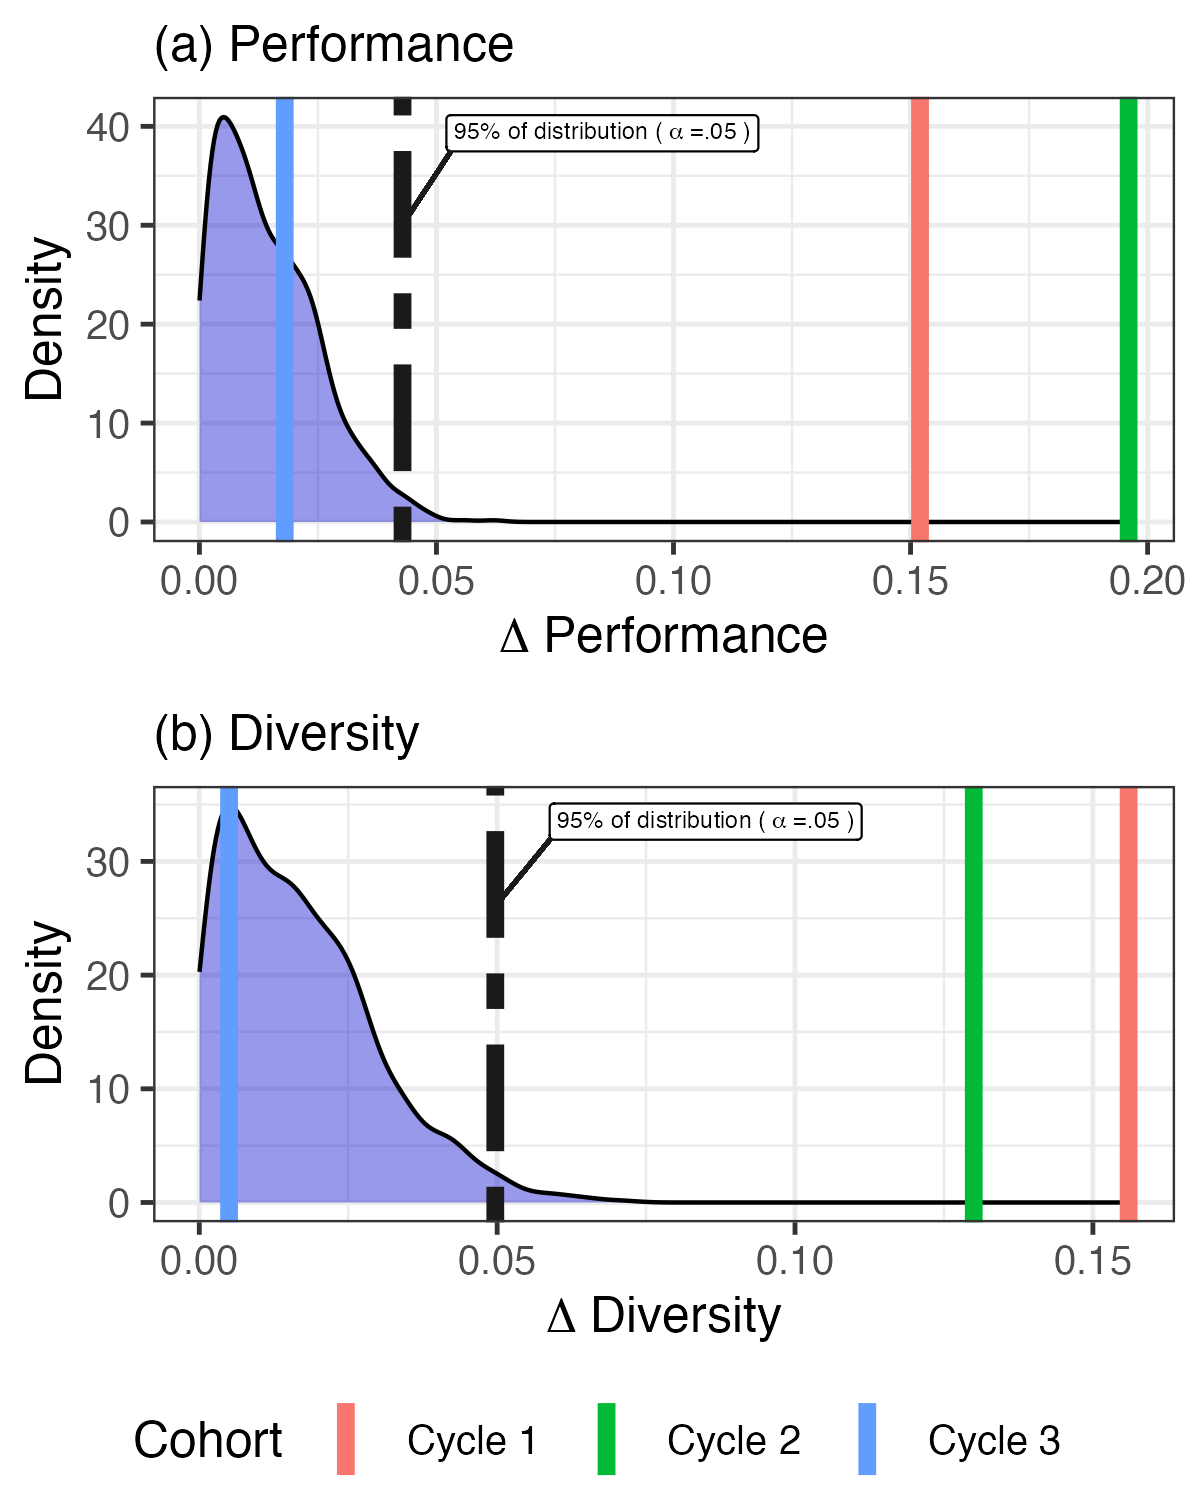
\includegraphics[width=.9\textwidth,height=\textheight,keepaspectratio]{results/figures/permutation_tests.png} 
        \begin{notes}
        This figure displays the distributions of differences in project performance (panel a) and diversity (panel b) from 1000 randomly drawn pairs of potential cohorts from application cycle 1. The dashed black vertical line represents the 95 percentile of these differences. The solid vertical lines represent the max pareto gain on performance (panel a) and diversity (panel b) in each application year.
        \end{notes}
    \end{figure}
    
    \newpage
    \begin{figure}[!htb]
    \centering
        \caption{Project Quality by Deciles of Alternative Screening Scores (Cycle 1)} \label{fig:alt_talent_dist}
      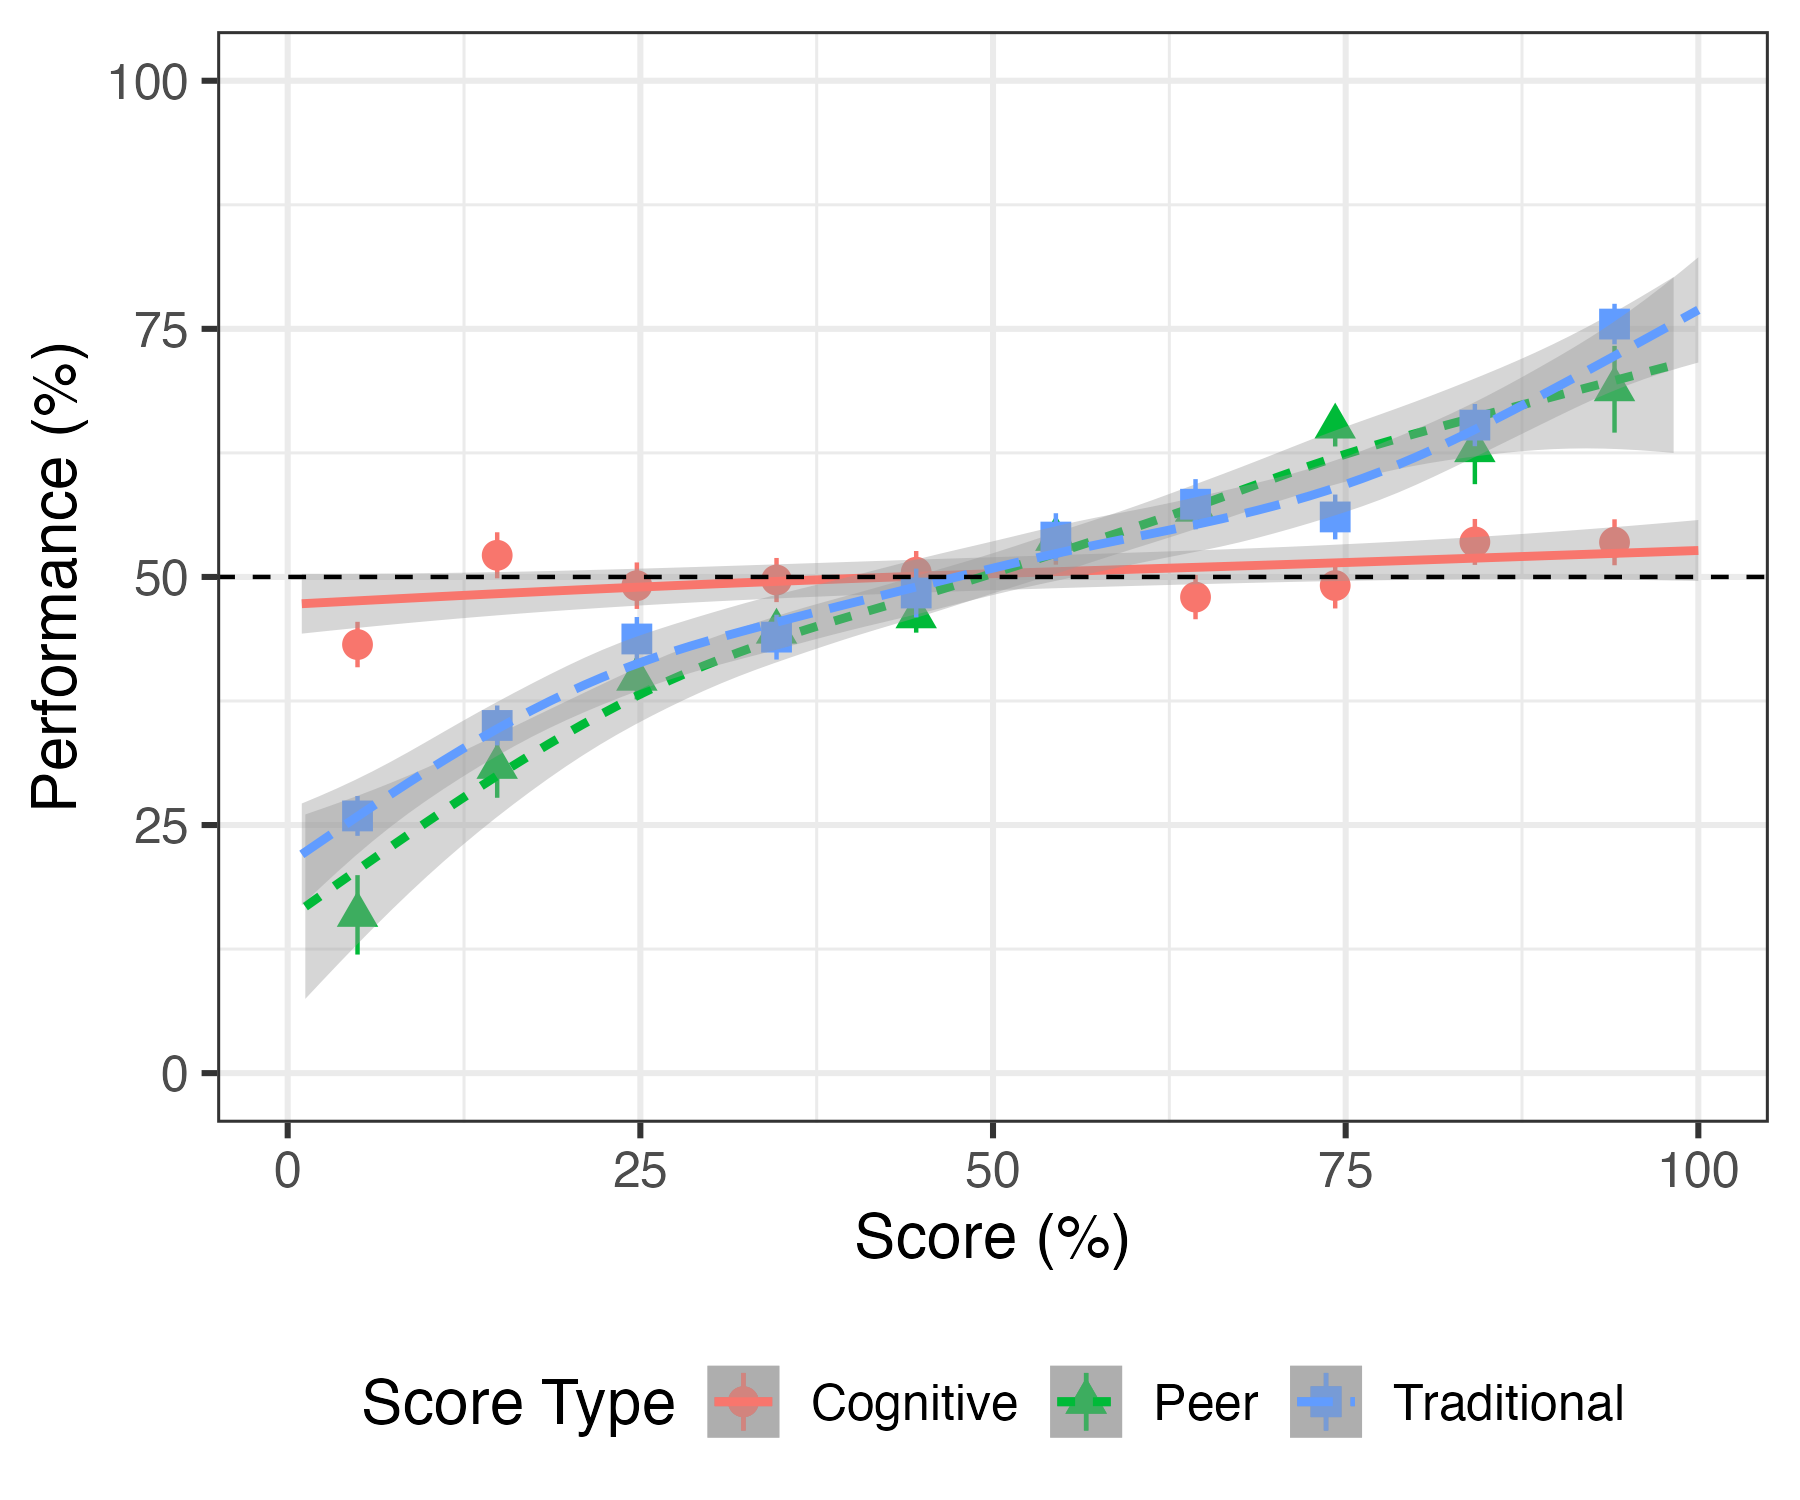
\includegraphics[width=\textwidth,height=\textheight,keepaspectratio]{\figurepath/pq_by_scores_c1.png} 
        \begin{notes}
        This figure plots the percentile of average expert-judged project quality (i.e. performance) by deciles of cognitive, peer, and traditional scores for the cycle 1 cohort. The cognitive score is the percentile of the candidate's IQ, the peer score is the percentile of the average peer assessment of each applicant video, and the traditional score is the average percentile of a candidate's IQ and project essay rating.   
        \end{notes}
    \end{figure}
    
    \newpage
    \begin{figure}[!htb]
    \centering
        \caption{Socioeconomic (Dis)Advantage by Deciles of Alternative Screening Scores (Cycle 1)} \label{fig:disadvantage_corr}
      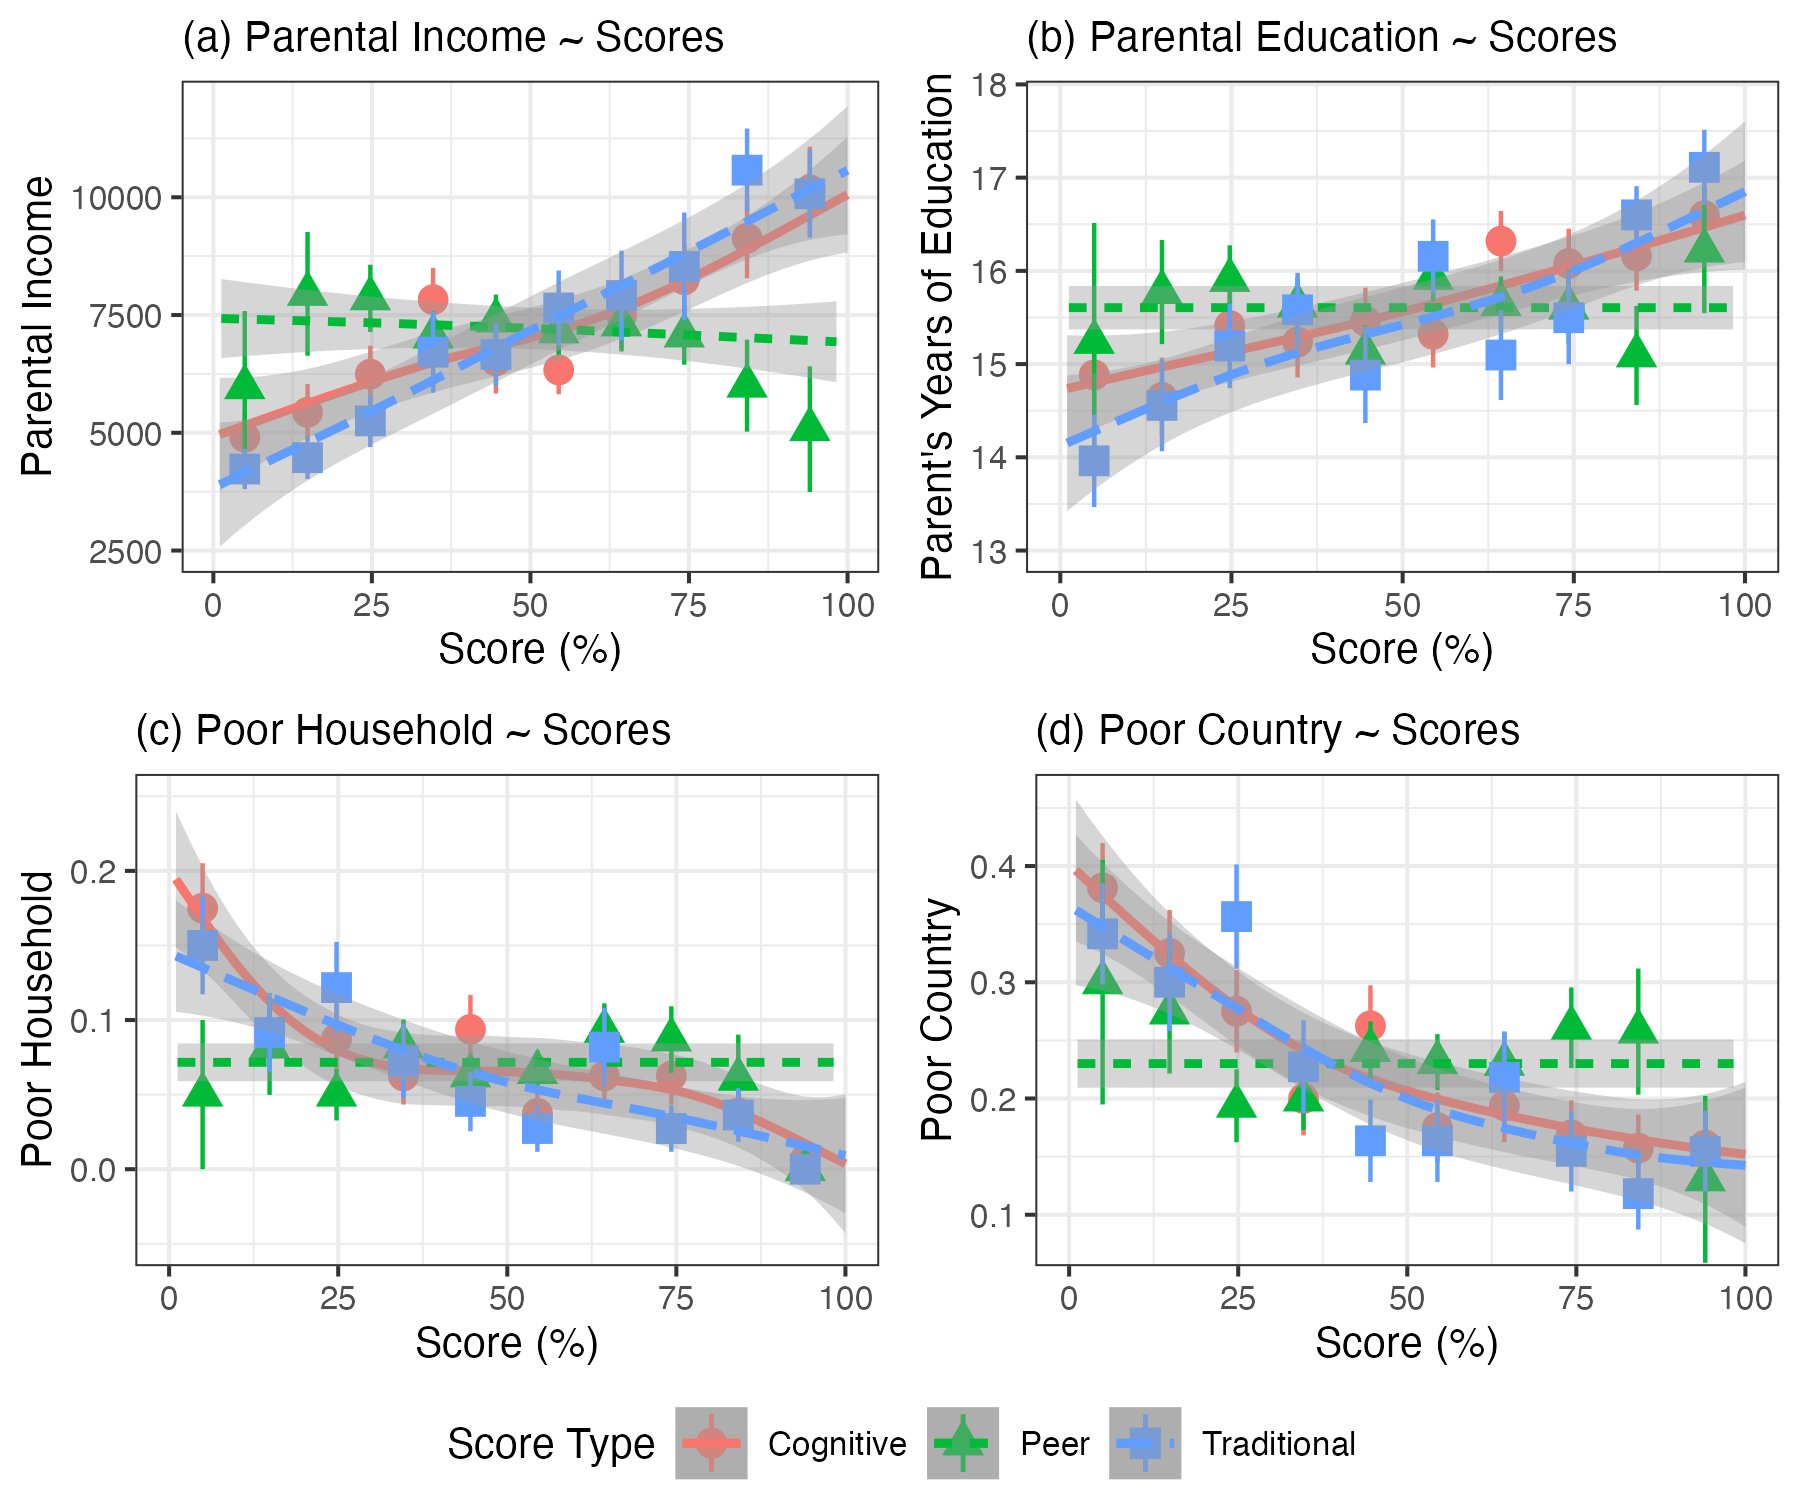
\includegraphics[width=\textwidth,height=\textheight,keepaspectratio]{results/figures/disadvantage_by_scores.png} 
        \begin{notes}
        This figure plots the average of various measures of applicant socioeconomic (dis)advantage by deciles of cognitive, peer, and traditional scores for the cycle 1 cohort. The measures of (dis)advantage from Panel A to D in order are predicted mean parent income (yearly), years of education of most educated parent, whether or not the applicant lives in a globally poor household (mean parent income less than \$1,000 a year), and whether or not the applicant lives in a poor country (less than \$12,000 GDP per capita). The cognitive score is the percentile of the candidate's IQ, the peer score is the percentile of the average peer assessment of each applicant video, and the traditional score is the average percentile of a candidate's IQ and project essay rating.   
        \end{notes}
    \end{figure}
    
    \newpage
    \begin{figure}[!htb]
    \centering
        \caption{Comparing Alternative Selection Strategies} \label{fig:alt_screen}
      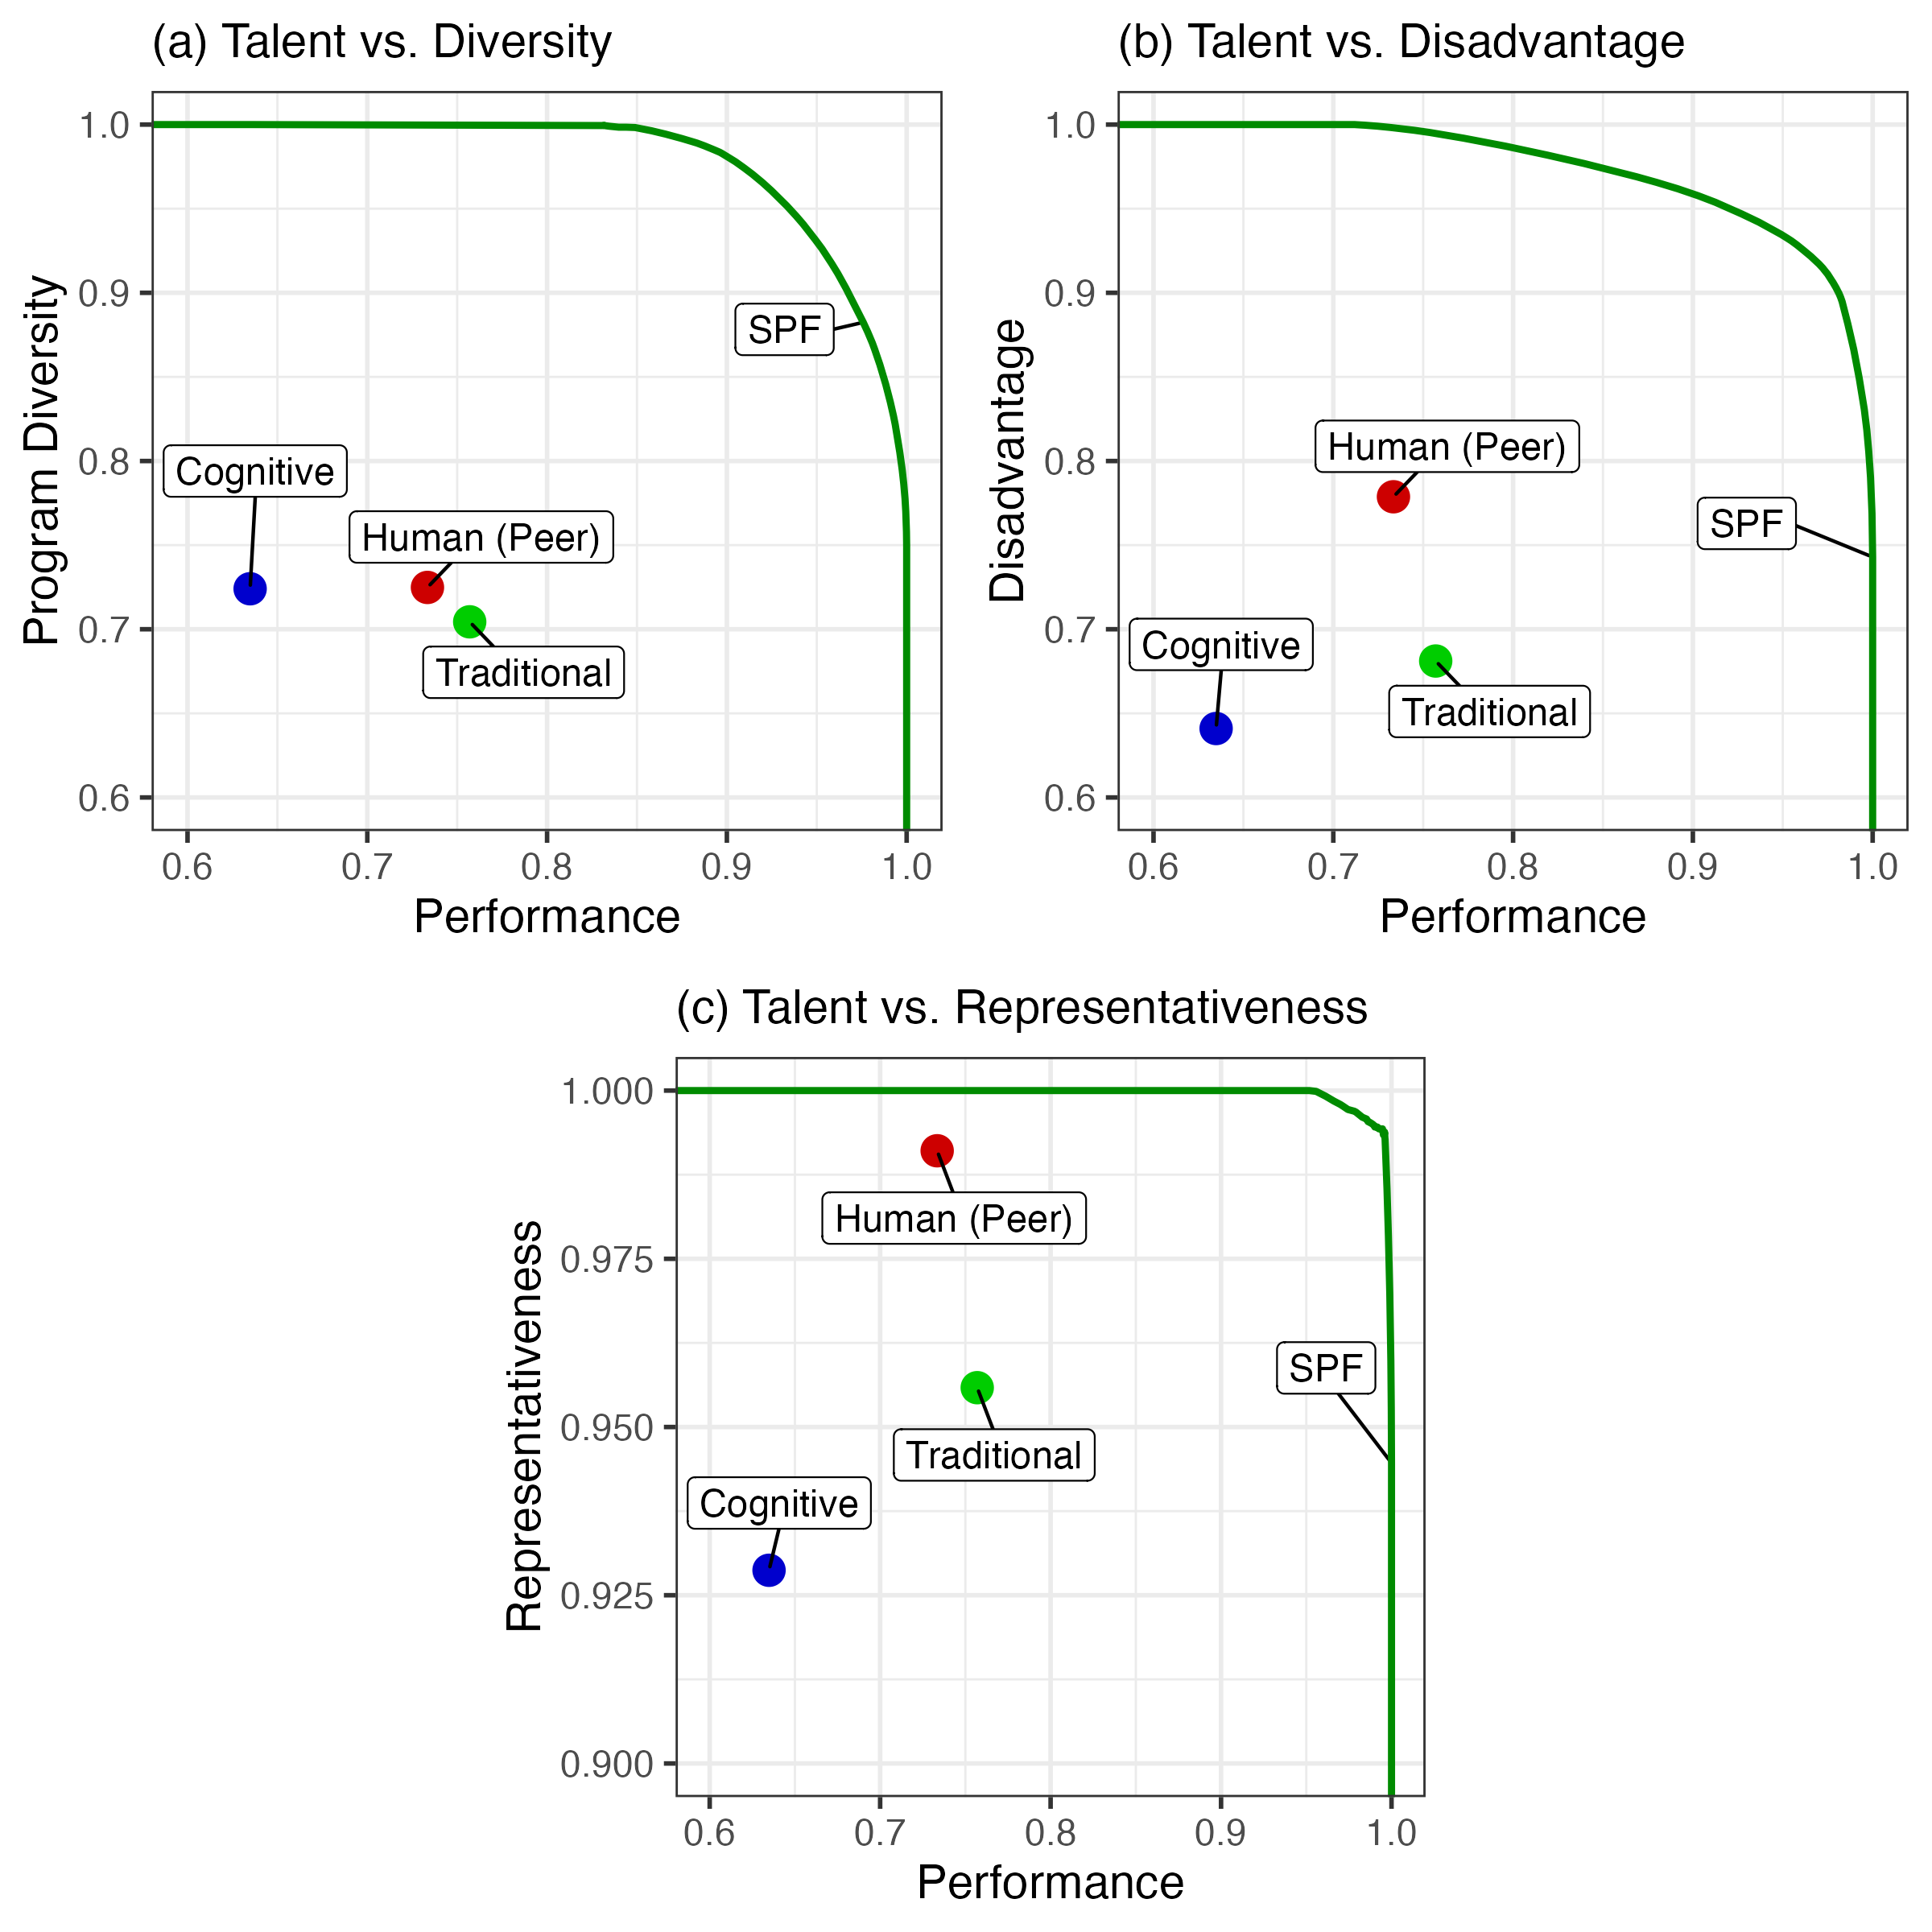
\includegraphics[width=\textwidth,height=\textheight,keepaspectratio]{results/figures/alt_screening_performance.png} 
        \begin{notes}
        This figure displays various SPF estimates for the  finalist cohort using the program's notion of diversity (Panel a), a disadvantage notion of diversity (Panel b), and a representativeness notion of diversity (Panel c). The y-axes represent diversity scores while the x-axes represent average cohort performance (i.e. project scores). The green curves are our estimates of three alternative cycle 1 SPFs, which are estimates the upper bound of diversity that is achievable at every level of cohort performance. Each dot represents the performance and diversity of cohorts had they been selected using those with the highest cognitive (blue), traditional (green), or peer (red) scores.  Each dot represents the performance and diversity of cohorts had they been selected using only cognitive ability (blue), a combination of written essay judgements and cognitive ability (aka a "traditional" score, which is green), and just peer review (red).
        \end{notes}
    \end{figure}
    
    \newpage
    \begin{figure}[!htb]
    \centering
        \caption{Comparing Diversity Tradeoffs for Different Performance Measures} \label{fig:compare_div_tradeoffs}
      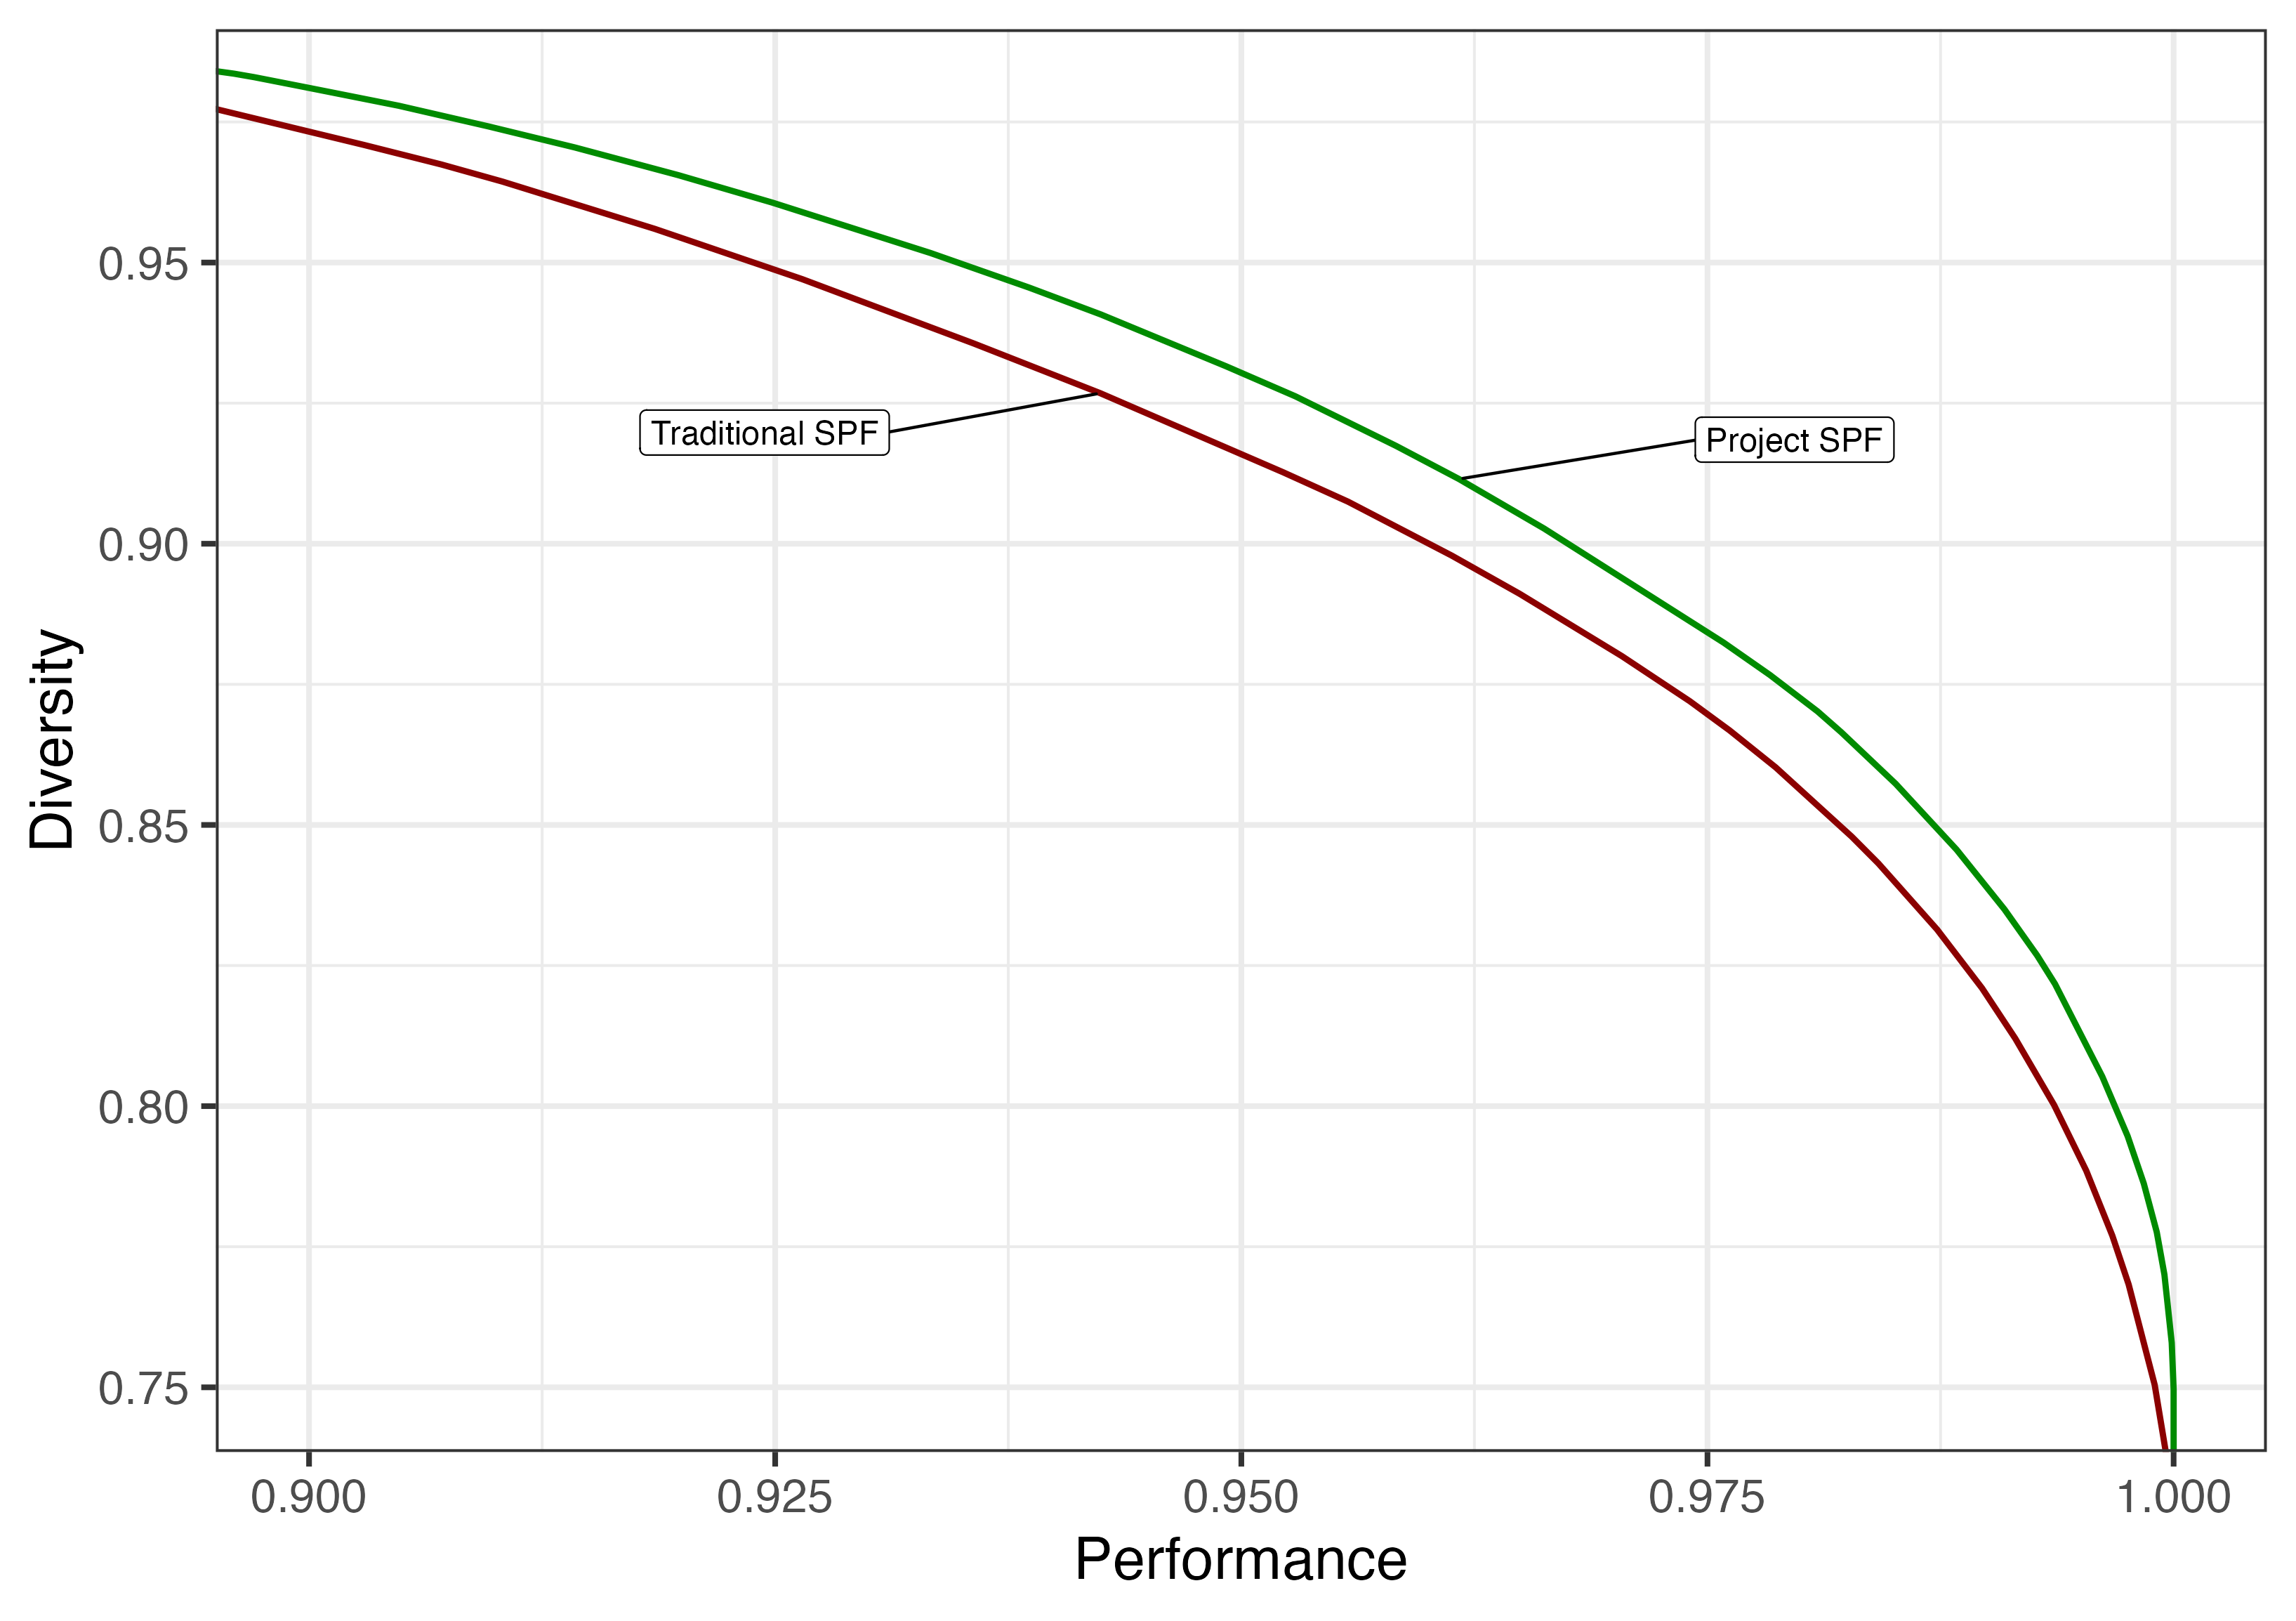
\includegraphics[width=\textwidth,height=\textheight,keepaspectratio]{results/figures/alt_merit_spfs.png} 
        \begin{notes}
        This figure displays the SPF we estimated for the cycle 1 finalist cohort and an SPF based on a more traditional method of measuring performance (i.e. the average of cognitive ability and an essay assessment). The y-axis represents the diversity score while the x-axis represents average cohort performance on projects or the traditional score. The vertical distance between the SPFs represents the difference in maximal diversity conditional on a cohort performing at a particular percentile of both scores. 
        \end{notes}
    \end{figure}
    
    \newpage
    
\begin{table}[htbp] 
    \centering 
    \caption{Summary Statistics:  Program Applicants. Raw data come from surveys completed by applicants. Data are pooled across three application years.}
    \label{tab:pooled_demo}
    \begin{tabular}{@{\extracolsep{5pt}}lccccc} 
    \\[-1.8ex]\hline 
    \hline \\[-1.8ex] 
    \emph{Panel A: Demographics} & \multicolumn{1}{c}{N} & \multicolumn{1}{c}{Mean} & \multicolumn{1}{c}{St. Dev.} & \multicolumn{1}{c}{Min} & \multicolumn{1}{c}{Max} \\ 
    \hline \\[-1.8ex] 
    Male & 5,772 & 0.41 & 0.49 & 0 & 1 \\ 
    Age & 5,770 & 16.43 & 0.81 & 15 & 18 \\ 
    Poor Country & 5,720 & 0.42 & 0.49 & 0 & 1 \\ 
    Poor Household & 5,772 & 0.18 & 0.38 & 0 & 1 \\ 
    Yrs of Parent Education & 5,772 & 15.21 & 4.45 & 0 & 20 \\ 
    Mean Parent Income (\$) & 5,772 & 18,891 & 39,617 & 227 & 250,000 \\ 
    \hline
    & & & & & \\
    \emph{Panel B: Global Region} & \multicolumn{1}{c}{N} & \multicolumn{1}{c}{Mean} & \multicolumn{1}{c}{St. Dev.} & \multicolumn{1}{c}{Min} & \multicolumn{1}{c}{Max} \\ 
    \hline
    Latin America & 5,770 & 0.25 & 0.43 & 0 & 1 \\ 
    Sub-Saharan Africa & 5,770 & 0.20 & 0.40 & 0 & 1 \\ 
    Middle East & 5,770 & 0.18 & 0.38 & 0 & 1 \\ 
    Canada/US/UK+ & 5,770 & 0.14 & 0.35 & 0 & 1 \\ 
    India & 5,770 & 0.08 & 0.27 & 0 & 1 \\ 
    East Asia & 5,770 & 0.06 & 0.23 & 0 & 1 \\ 
    Western Europe & 5,770 & 0.04 & 0.20 & 0 & 1 \\ 
    Eastern Europe & 5,770 & 0.04 & 0.20 & 0 & 1 \\ 
    Caribbean/Pacific Islands & 5,770 & 0.01 & 0.08 & 0 & 1 \\ 
    \hline \hline \\[-1.8ex] 
    \end{tabular} 
    \end{table} 
    
    \newpage
    \begin{table}[!htbp] \centering 
      \caption{Summary Statistics: Project Reviewers. Raw data come from surveys completed by applicants. Data are pooled across three application years.}\label{tab:pooled_rev_demo}
      \label{} 
    \begin{tabular}{@{\extracolsep{5pt}}lccccc} 
    \\[-1.8ex]\hline 
    \hline \\[-1.8ex] 
    \emph{Panel A: Demographics} & \multicolumn{1}{c}{N} & \multicolumn{1}{c}{Mean} & \multicolumn{1}{c}{St. Dev.} & \multicolumn{1}{c}{Min} & \multicolumn{1}{c}{Max} \\ 
    \hline \\[-1.8ex] 
    Male & 1,290 & 0.43 & 0.50 & 0 & 1 \\ 
    Age & 1,309 & 44.50 & 19.99 & 19 & 75 \\ 
    Poor Country & 1,321 & 0.46 & 0.50 & 0 & 1 \\ 
    \hline
    & & & & & \\
    \emph{Panel B: Global Region} & \multicolumn{1}{c}{N} & \multicolumn{1}{c}{Mean} & \multicolumn{1}{c}{St. Dev.} & \multicolumn{1}{c}{Min} & \multicolumn{1}{c}{Max} \\ 
    \hline
    Canada/US/UK+ & 1,334 & 0.37 & 0.48 & 0 & 1 \\ 
    India & 1,334 & 0.28 & 0.45 & 0 & 1 \\ 
    Western Europe & 1,334 & 0.07 & 0.25 & 0 & 1 \\ 
    Middle East & 1,334 & 0.07 & 0.26 & 0 & 1 \\ 
    Sub-Saharan Africa & 1,334 & 0.06 & 0.24 & 0 & 1 \\ 
    Latin America & 1,334 & 0.06 & 0.24 & 0 & 1 \\ 
    East Asia & 1,334 & 0.06 & 0.24 & 0 & 1 \\ 
    Eastern Europe & 1,334 & 0.01 & 0.12 & 0 & 1 \\ 
    Caribbean/Pacific Islands & 1,334 & 0.004 & 0.07 & 0 & 1 \\ 
    \hline \hline \\[-1.8ex] 
    \end{tabular} 
    \end{table} 